\chapter{Flavour Tagging}
\ChapFrame
\textit{This Appendix lists some additional results in support of Chapter \ref{chap-ftag}.}

\section{Understanding DIPS}\label{app-DIPS-perf}
\begin{figure}[h!]
  \center
  \begin{minipage}[c]{0.7\textwidth}
    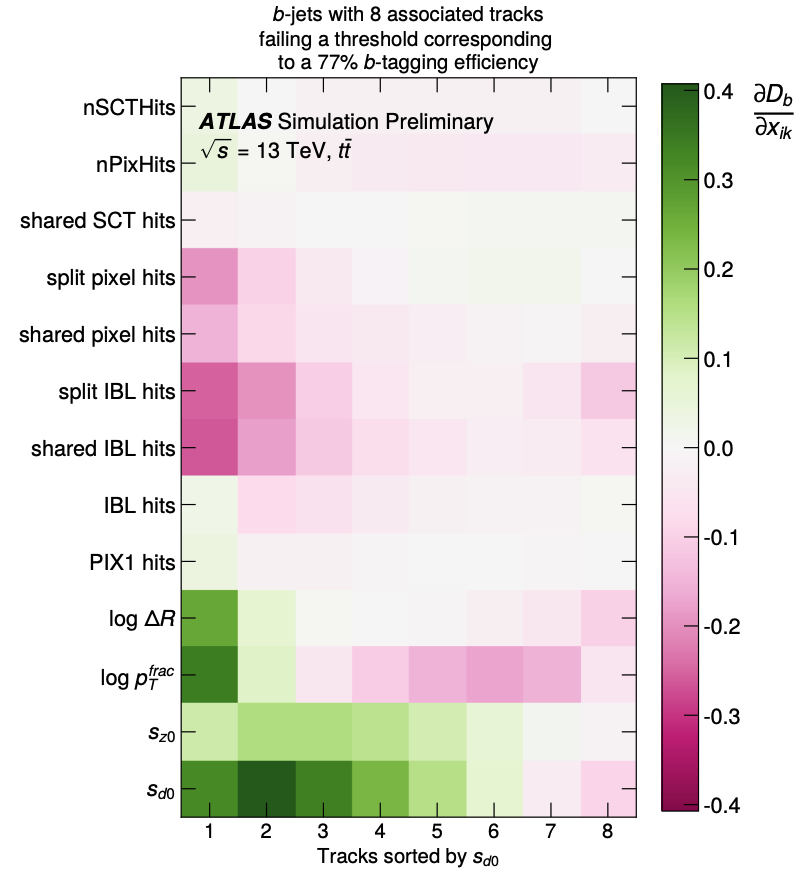
\includegraphics[width=\textwidth]{Images/FTAG/dipsSaliency.png}
  \end{minipage}
  \begin{minipage}[c]{0.25\textwidth}
    \caption{Saliency map for $b$-tagging with 8 tracks sorted by $|S_{d_0}|$ and indexed by $i$, showing the gradient of the discriminant $D_b$ with respect to the $k$ track features $x_{ik}$ \cite{ATL-PHYS-PUB-2020-014}.} 
  \label{fig:dipsSaliency}
  \end{minipage}
\end{figure}

How does \gls{dips} work under the hood? The interpretability of machine learning models is an active area of research. Several effective approaches exist to gauge the importance of the input on the prediction. Figure~\ref{fig:dipsSaliency} presents the result of applying the \textit{saliency maps} technique \cite{Simonyan2013DeepIC}. Using the $b$-tagging discriminant $D_b$ of Equation \ref{bdisc} at a fixed efficiency of 77\%, the average importance of each feature in the track inputs is assessed by averaging the gradient of the discriminant with respect to the track features over a set of $N$ jets with strictly 8 associated tracks failing the threshold:
\begin{equation}
  \frac{\partial D_b}{\partial x_{ik}} = \frac{1}{N} \sum_{j=1}^N \frac{\partial D_b^{j}}{\partial x_{ik}^{j}},
\end{equation} 
where $i$ indexes the 8 tracks, $j$ indexes the jet in the sample of size $N$, $x_{ik}$ is the $k^{th}$ feature of the $i^{th}$ track \cite{ATL-PHYS-PUB-2020-014}. This process effectively probes the linear sensitivity of the discriminant on the track features. Using the saliency map, one can infer what features to modify to correct the failed tag assigned to the $b$-jets sample. The most sensitive parameters are measured to be the \gls{ip} significances of the first five tracks, and the logarithm of the $p_T^{\textrm{frac}}$ and $\Delta R$ of the track with largest $|s_{d_0}|$. This observation is physically motivated by the dynamic of the harder fragmentation of $b$-quarks, compared to light- and $c$-quarks. Negative gradients are measured for shared and split hits observables, translating into a further incorrect discriminant under a linear increase of these features. This is also physically motivated, as higher counts can be traced back to denser event environments where random combinations of hits to form tracks are more likely. However, total hit counts in the different tracker layers have a small positive impact, as these correlate with the reconstruction of the \gls{ip} parameters.

\section{DIPS with Variable Radius Jets}\label{ap-DIPSVR}
This section of the Appendix displays more information on the variable radius (\gls{vr}) jet training of \gls{dips}. The samples distributions are shown in Figure \ref{apfig:vrjetdist}.

\begin{figure}[h!]
  \centering
  \begin{subfigure}[b]{0.98\textwidth}
      \centering
      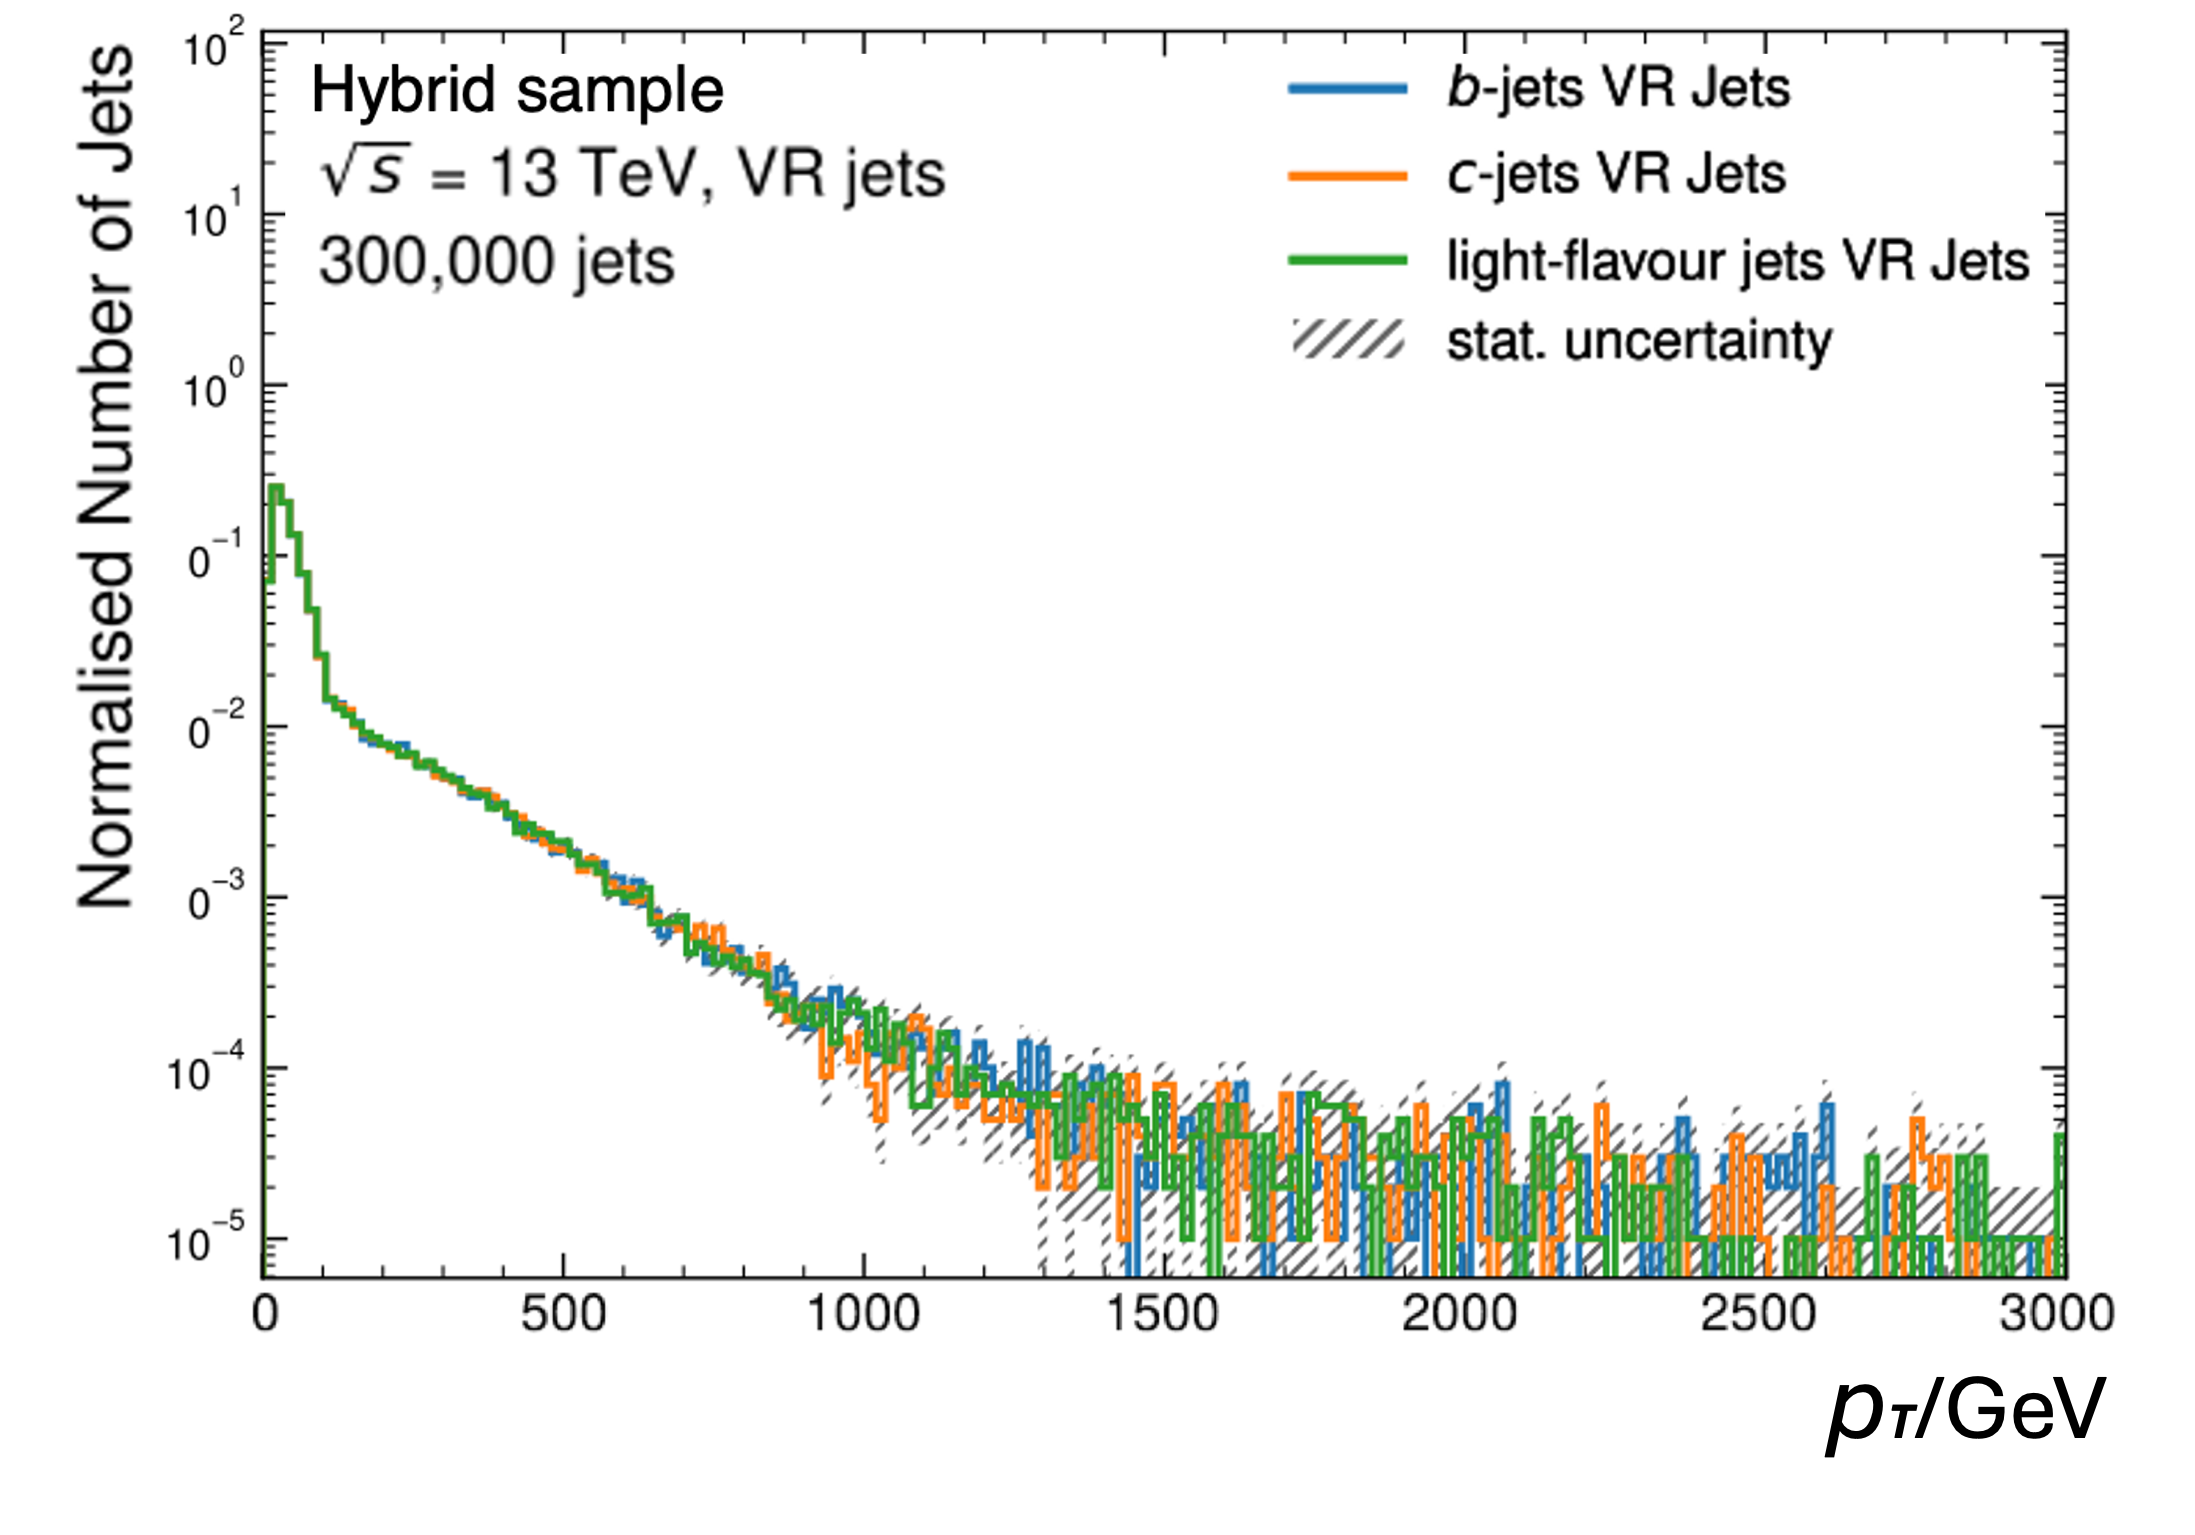
\includegraphics[width=0.48\textwidth]{Images/FTAG/VRDips/JetDist/hspt.png}
      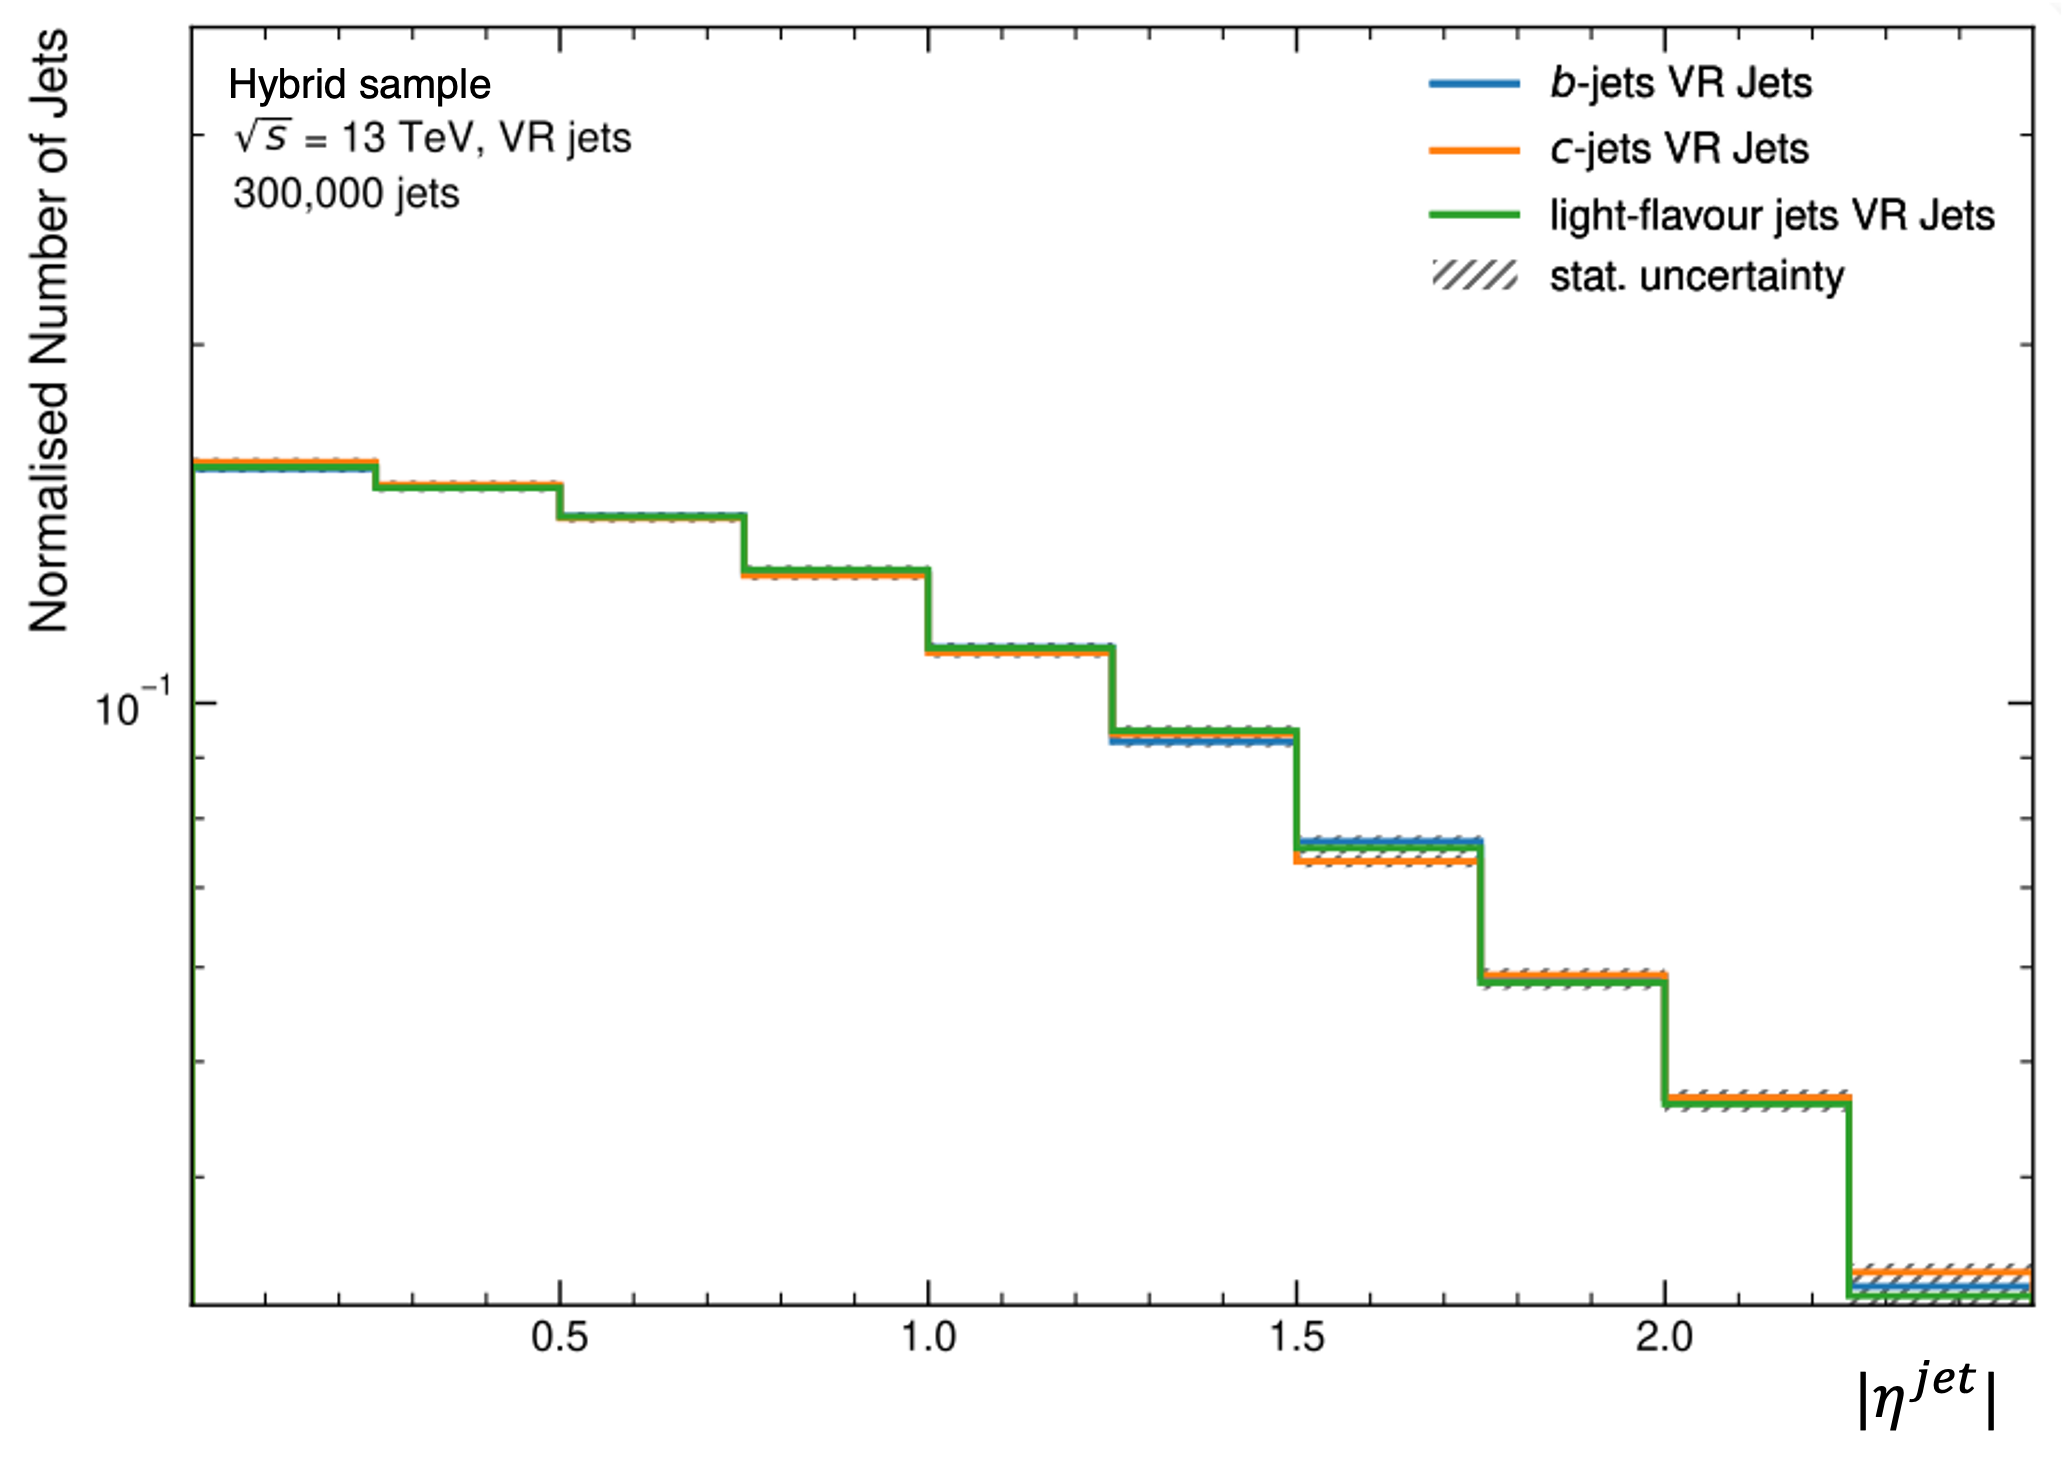
\includegraphics[width=0.48\textwidth]{Images/FTAG/VRDips/JetDist/hseta.png}
      \caption{Hybrid sample.} 
      \label{apfig:vrjetdisth}
  \end{subfigure}\\
  \begin{subfigure}[b]{0.98\textwidth}
      \centering
      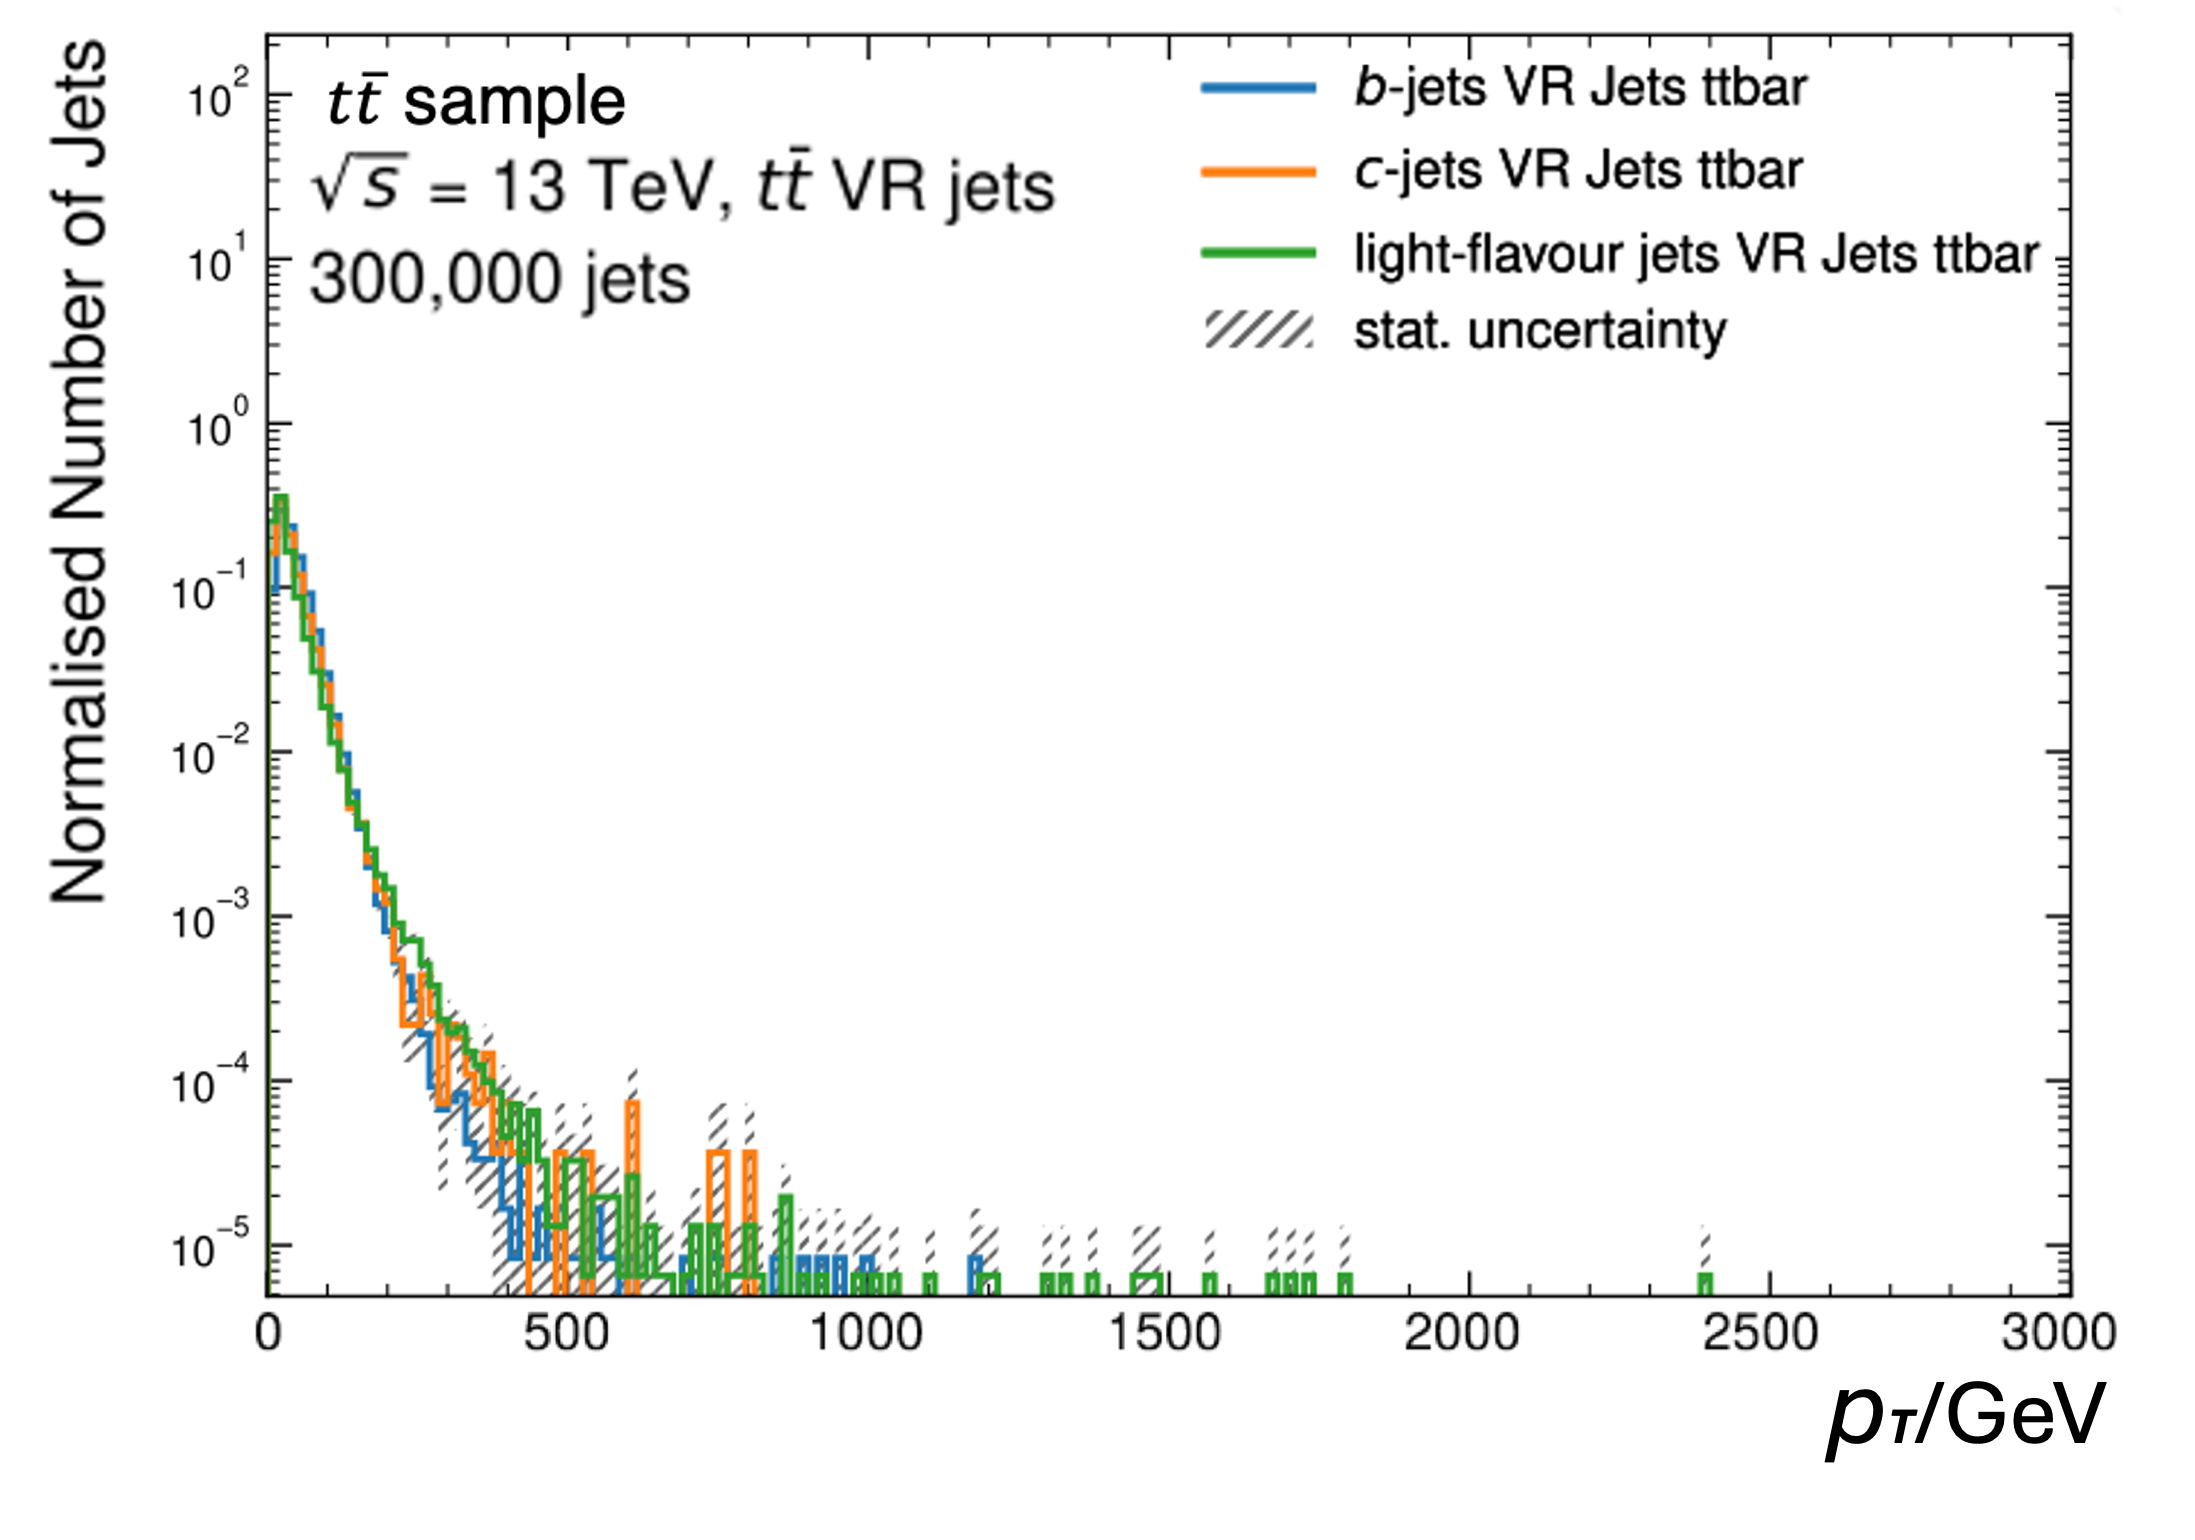
\includegraphics[width=0.48\textwidth]{Images/FTAG/VRDips/JetDist/ttpt.png}
      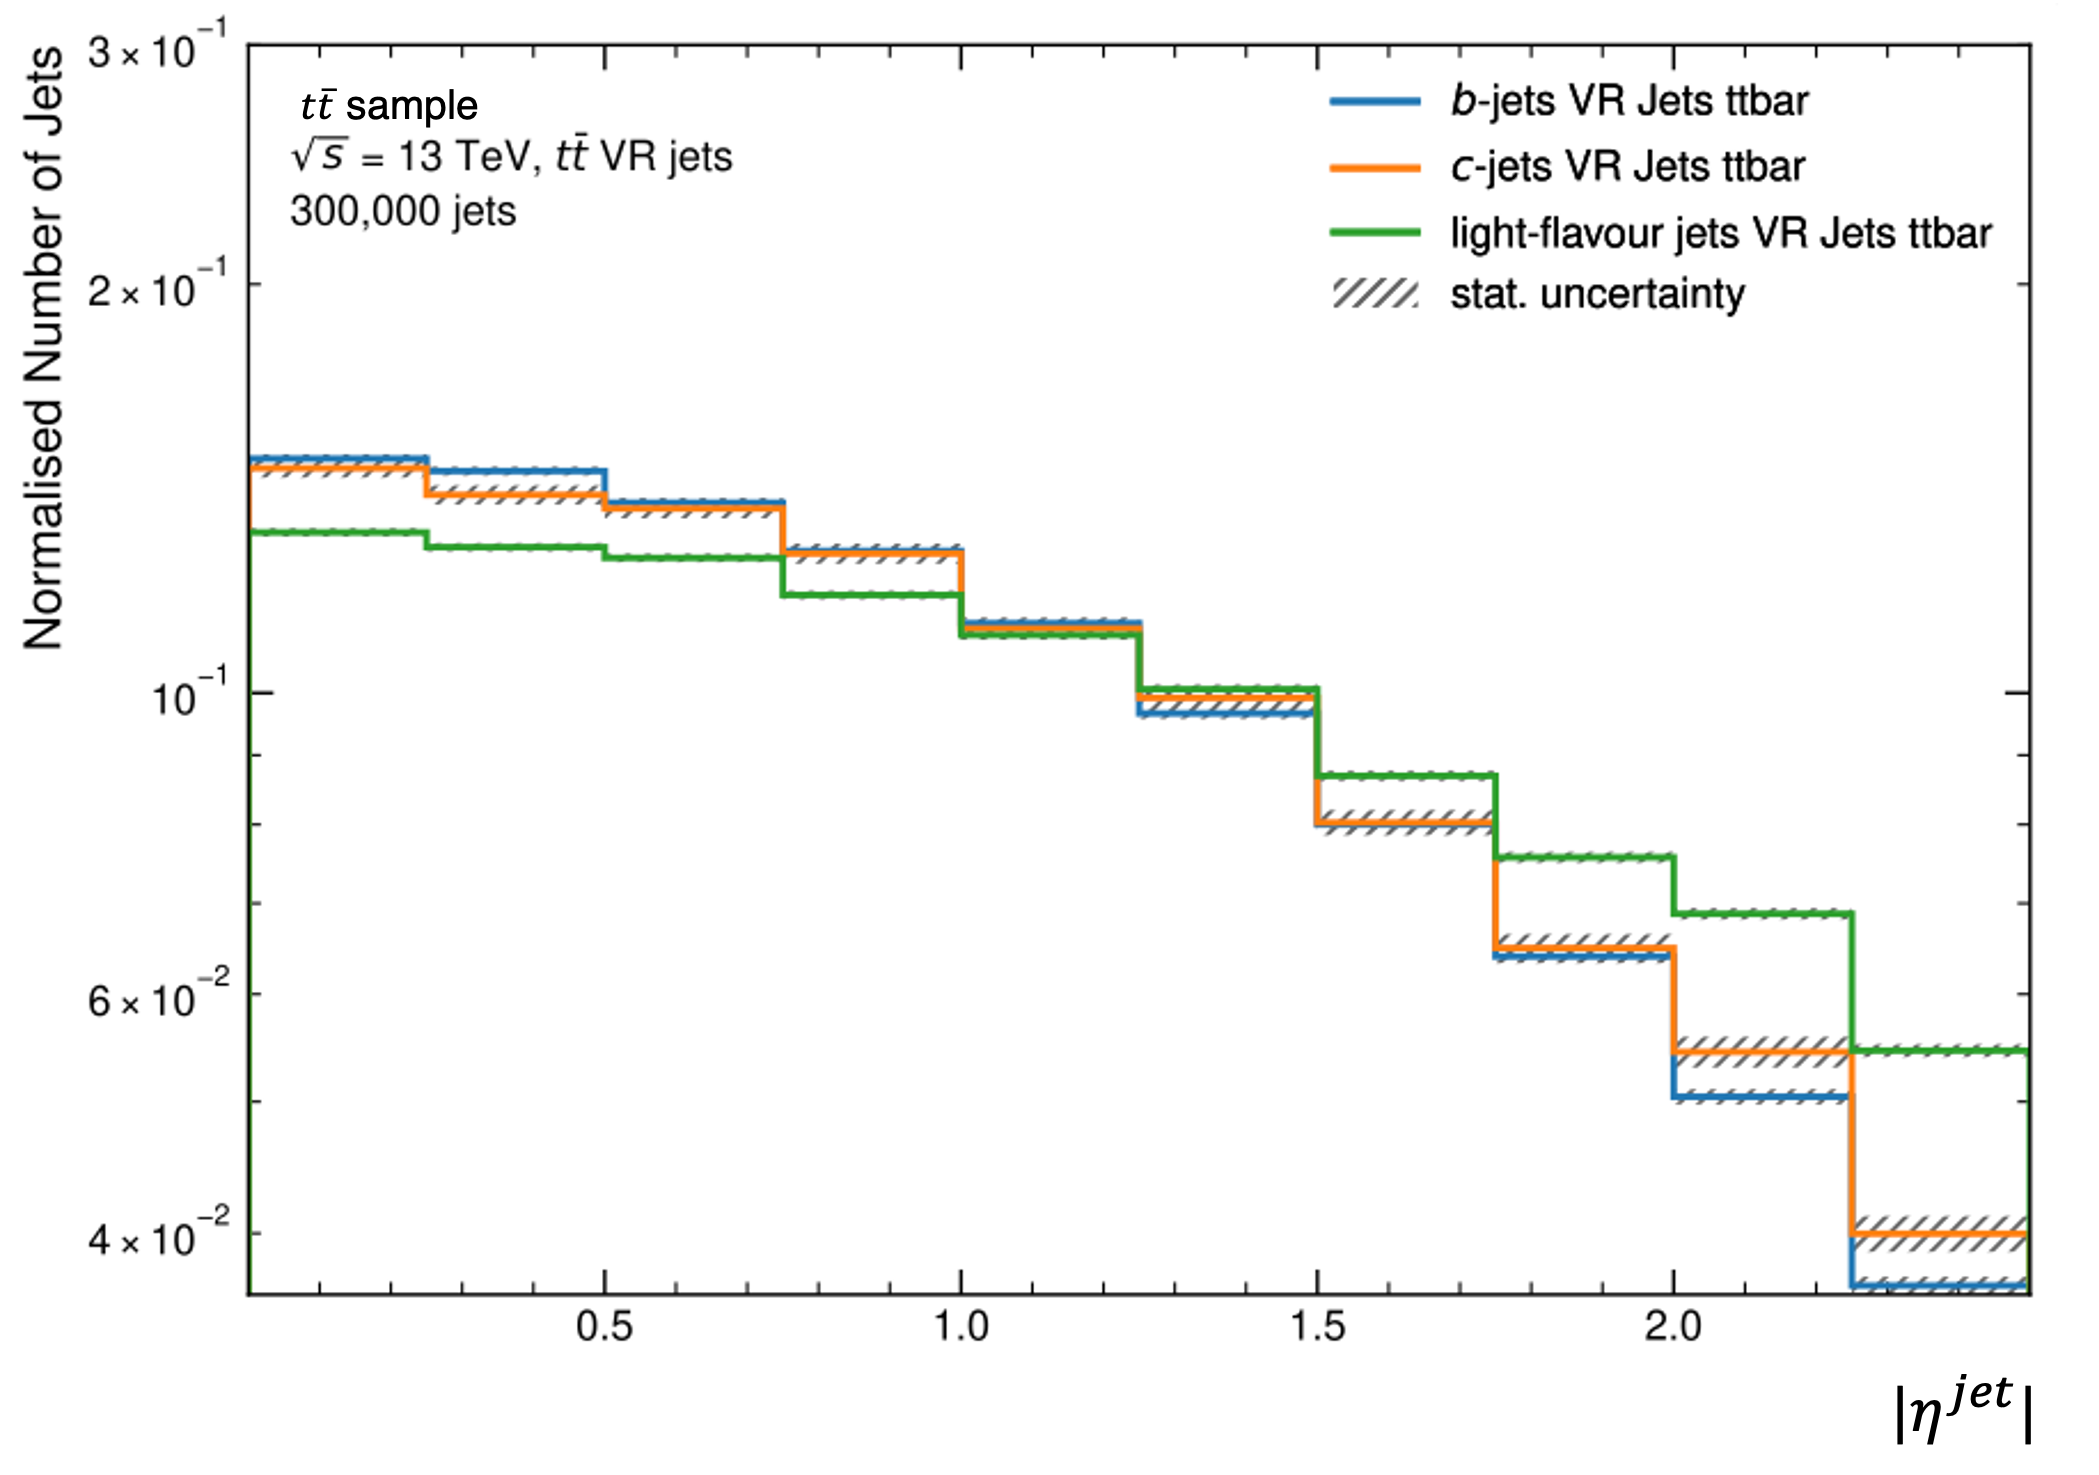
\includegraphics[width=0.48\textwidth]{Images/FTAG/VRDips/JetDist/tteta.png}
      \caption{$t\bar{t}$ sample.} 
      \label{apfig:vrjetdistt}
  \end{subfigure}\\
  \begin{subfigure}[b]{0.98\textwidth}
      \centering
      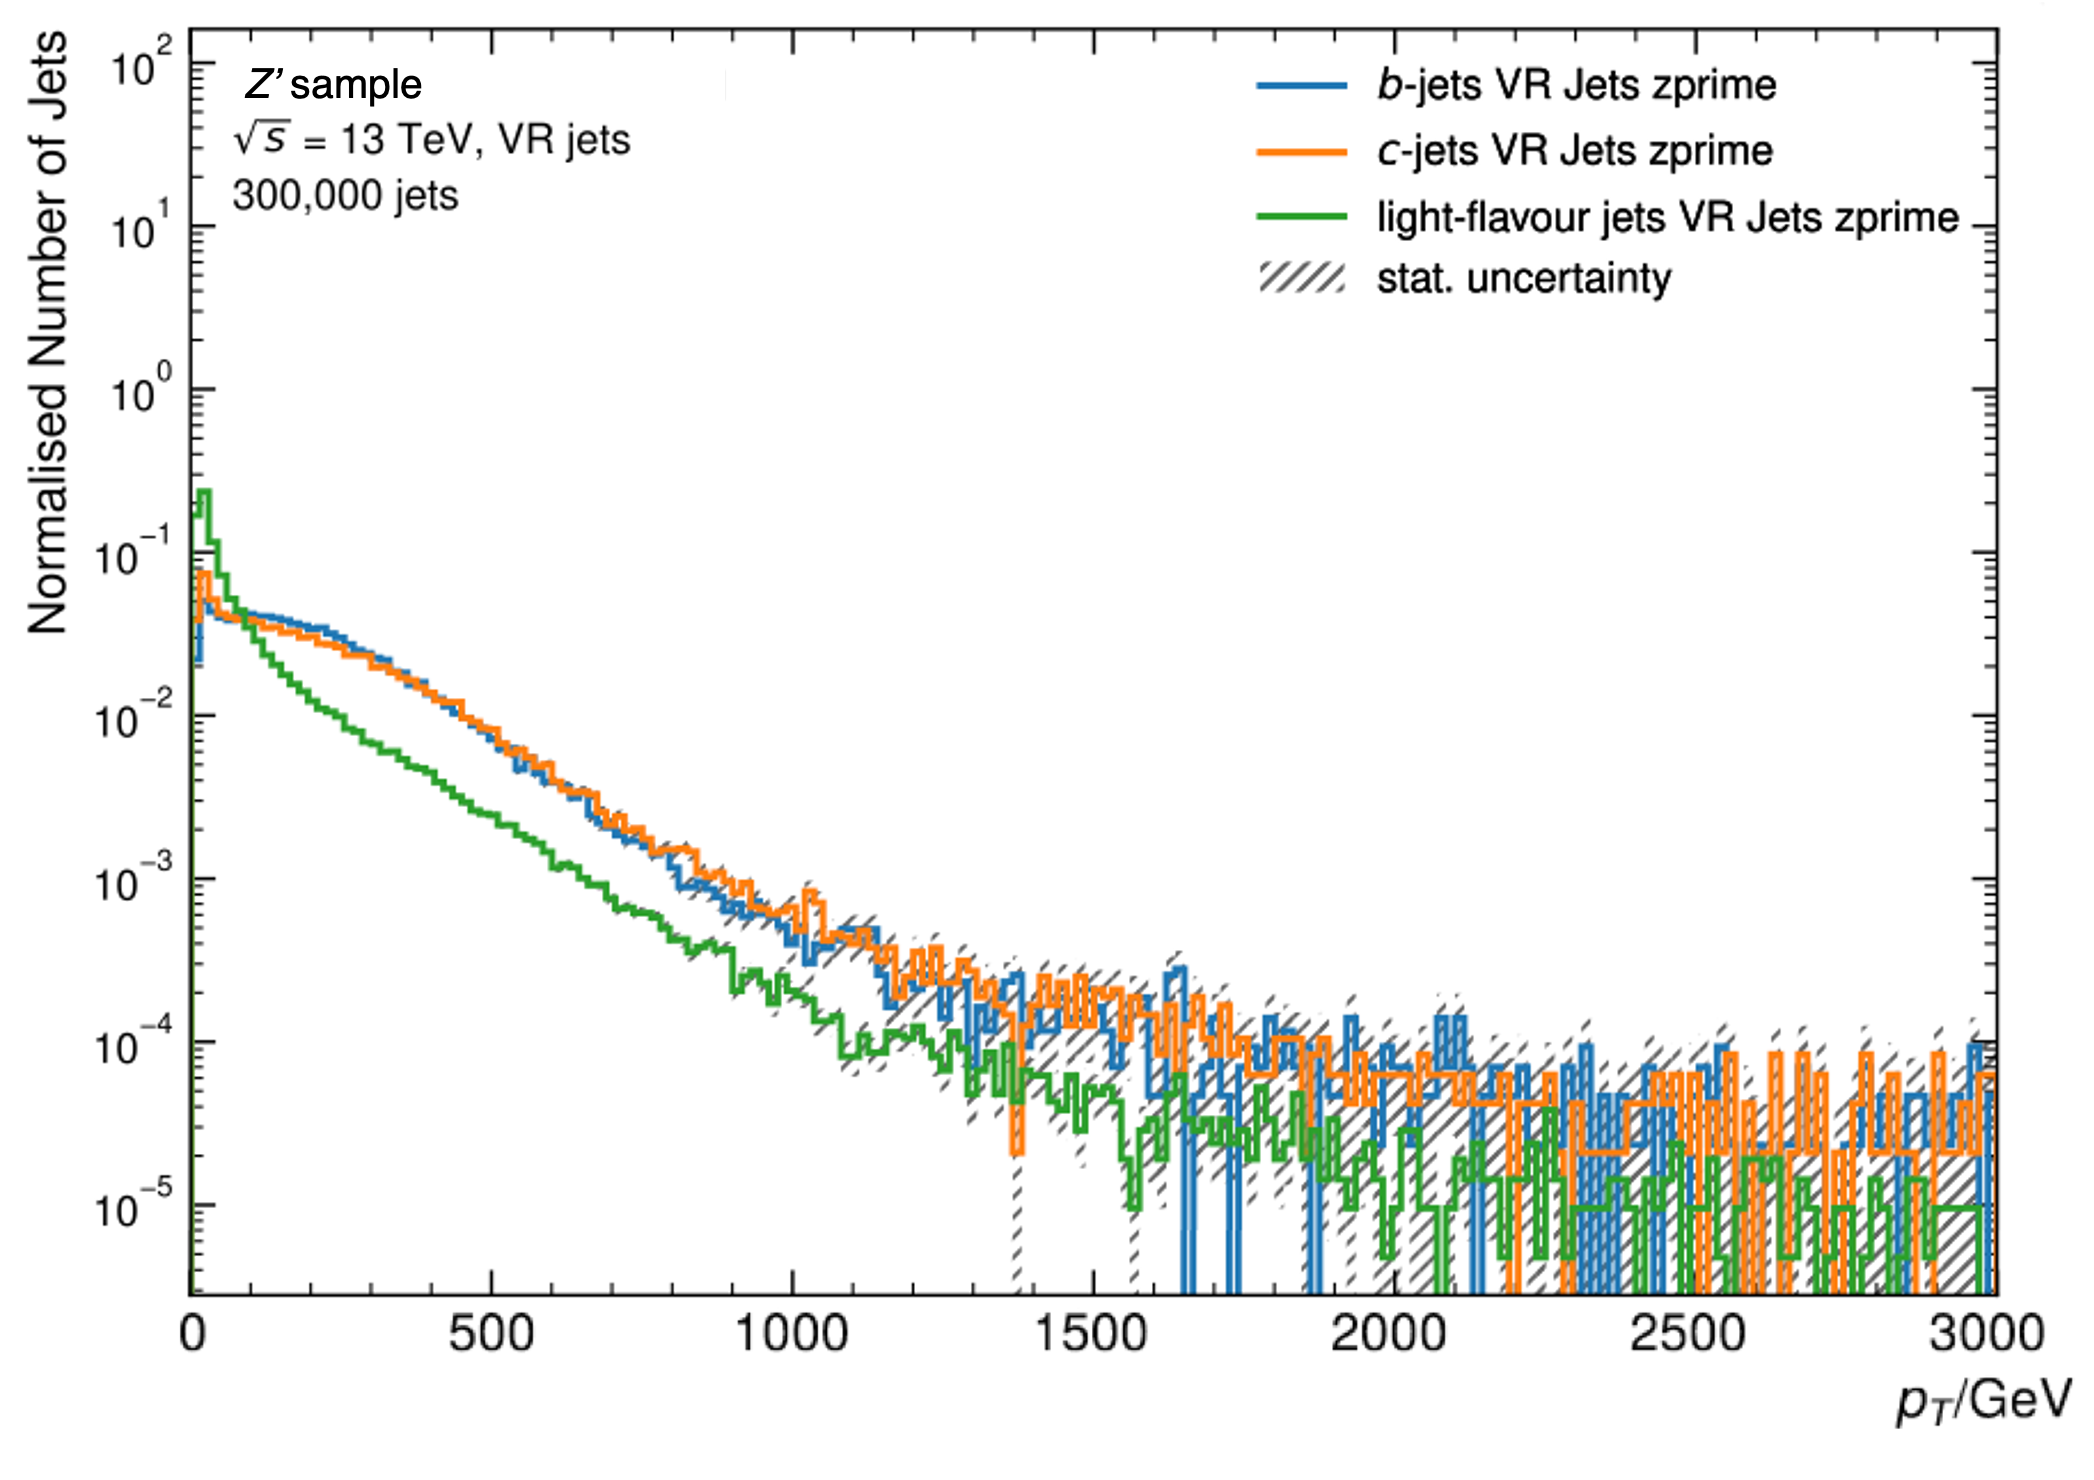
\includegraphics[width=0.48\textwidth]{Images/FTAG/VRDips/JetDist/zppt.png}
      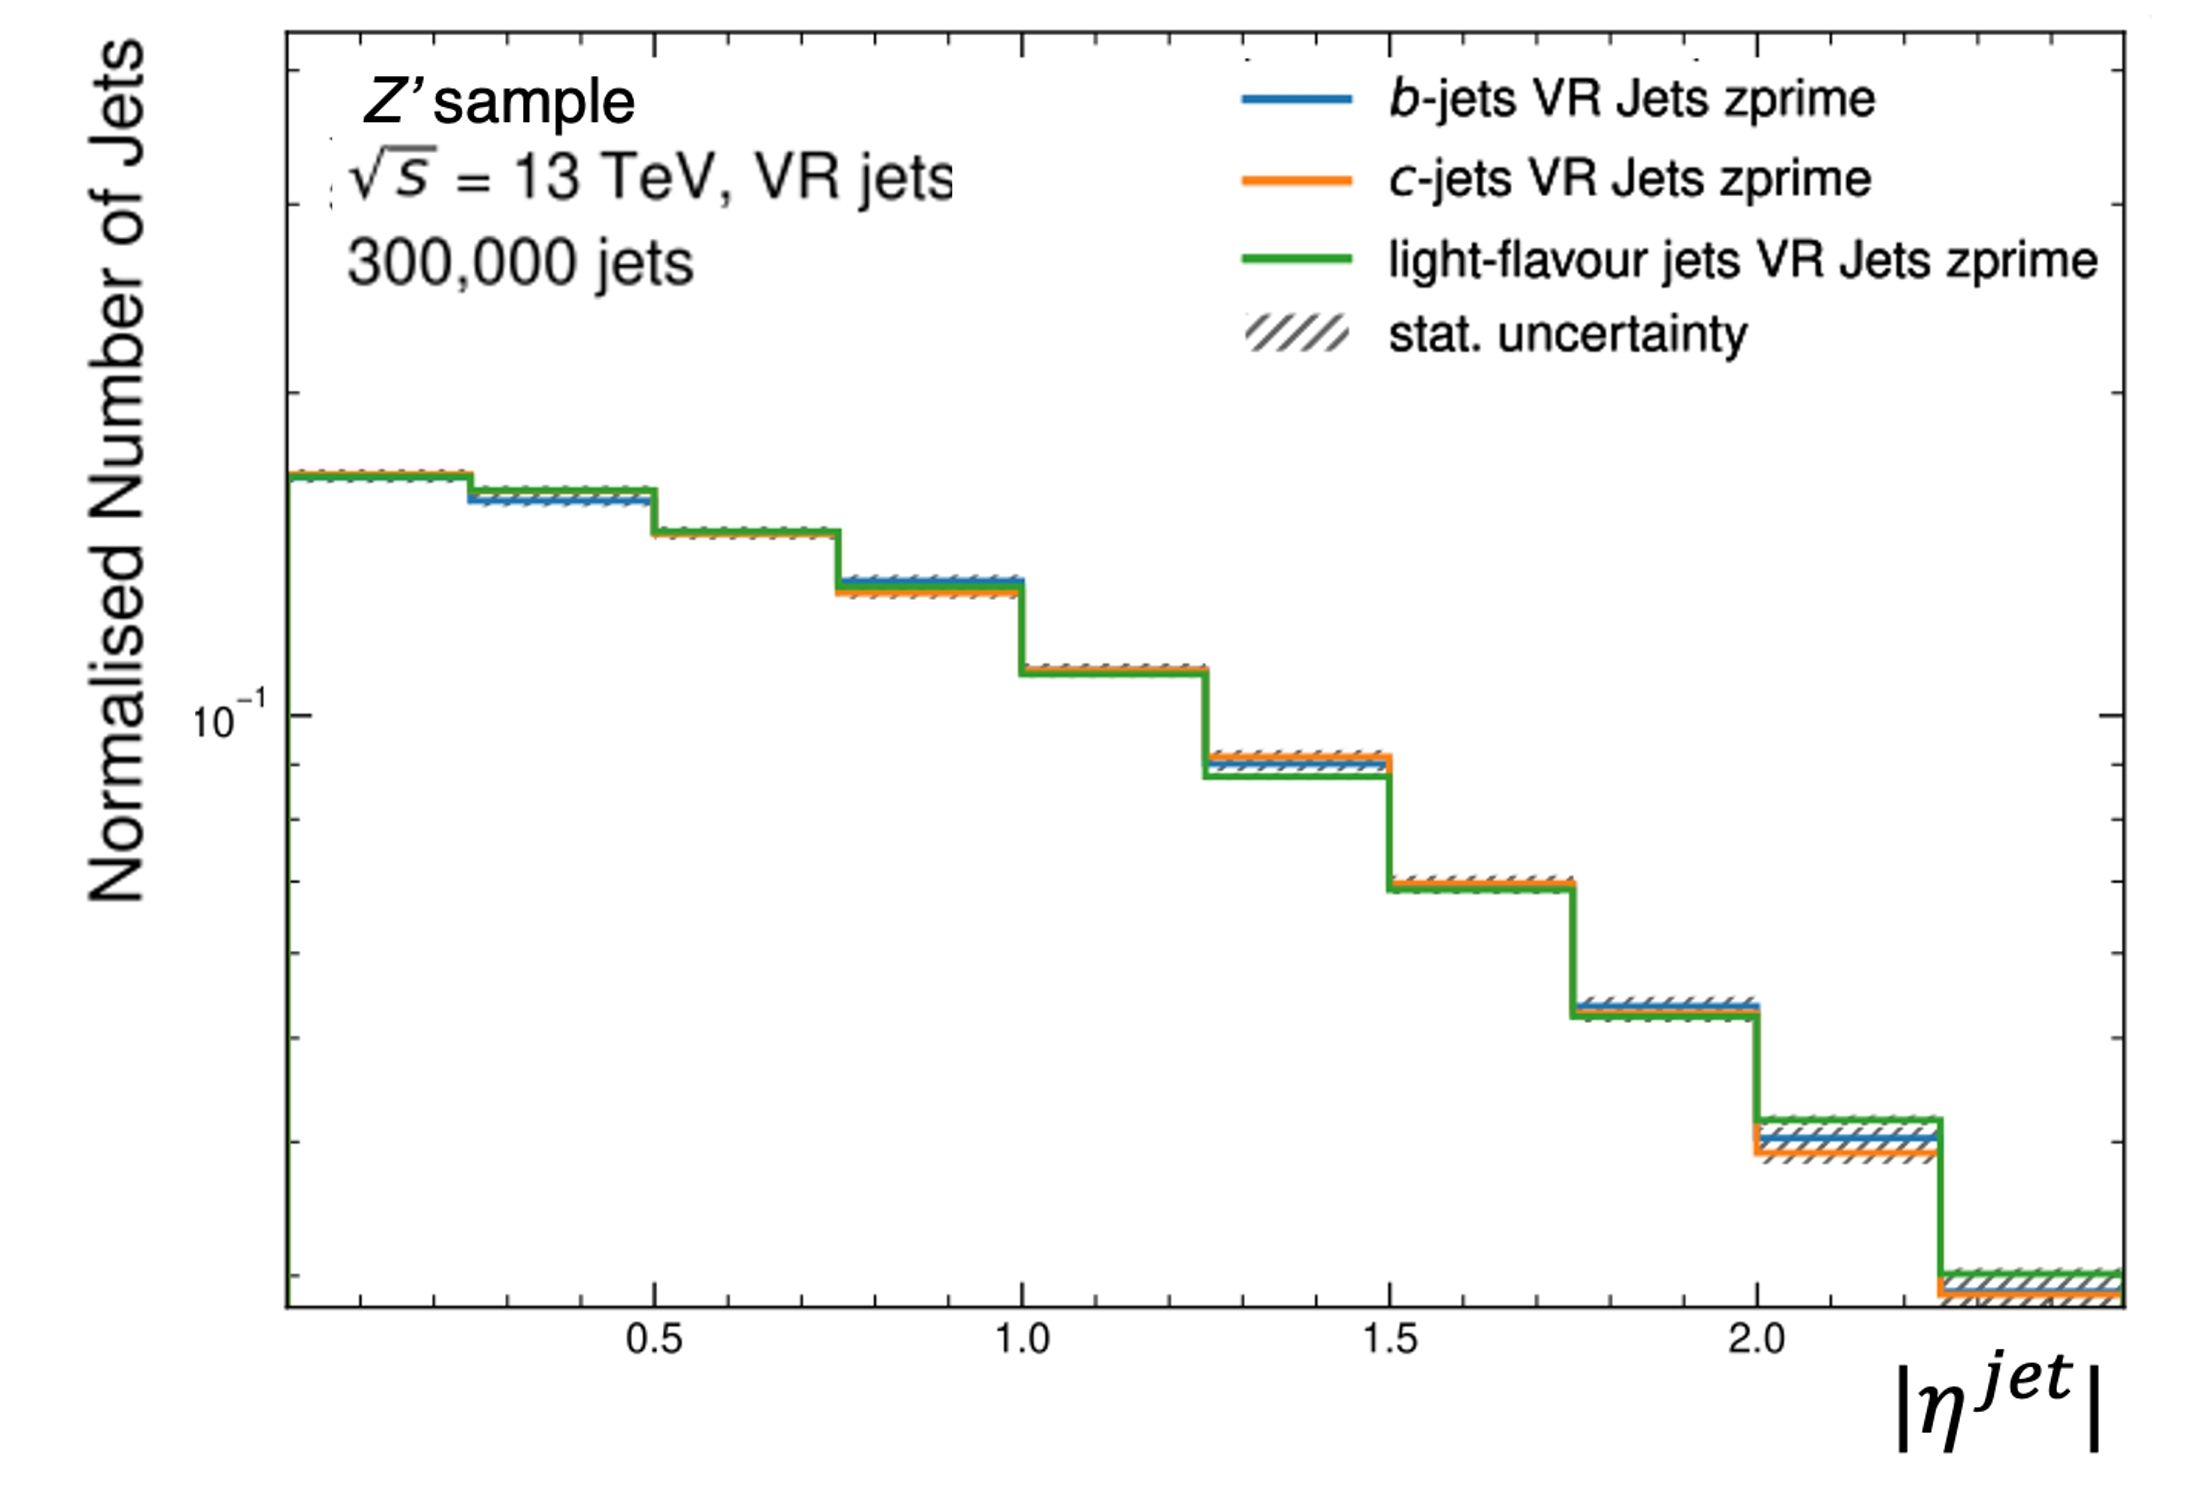
\includegraphics[width=0.48\textwidth]{Images/FTAG/VRDips/JetDist/zpeta.png}
      \caption{$Z'$ sample.} 
      \label{apfig:vrjetdiszp}
  \end{subfigure}\\
  \begin{subfigure}[b]{0.98\textwidth}
      \centering
      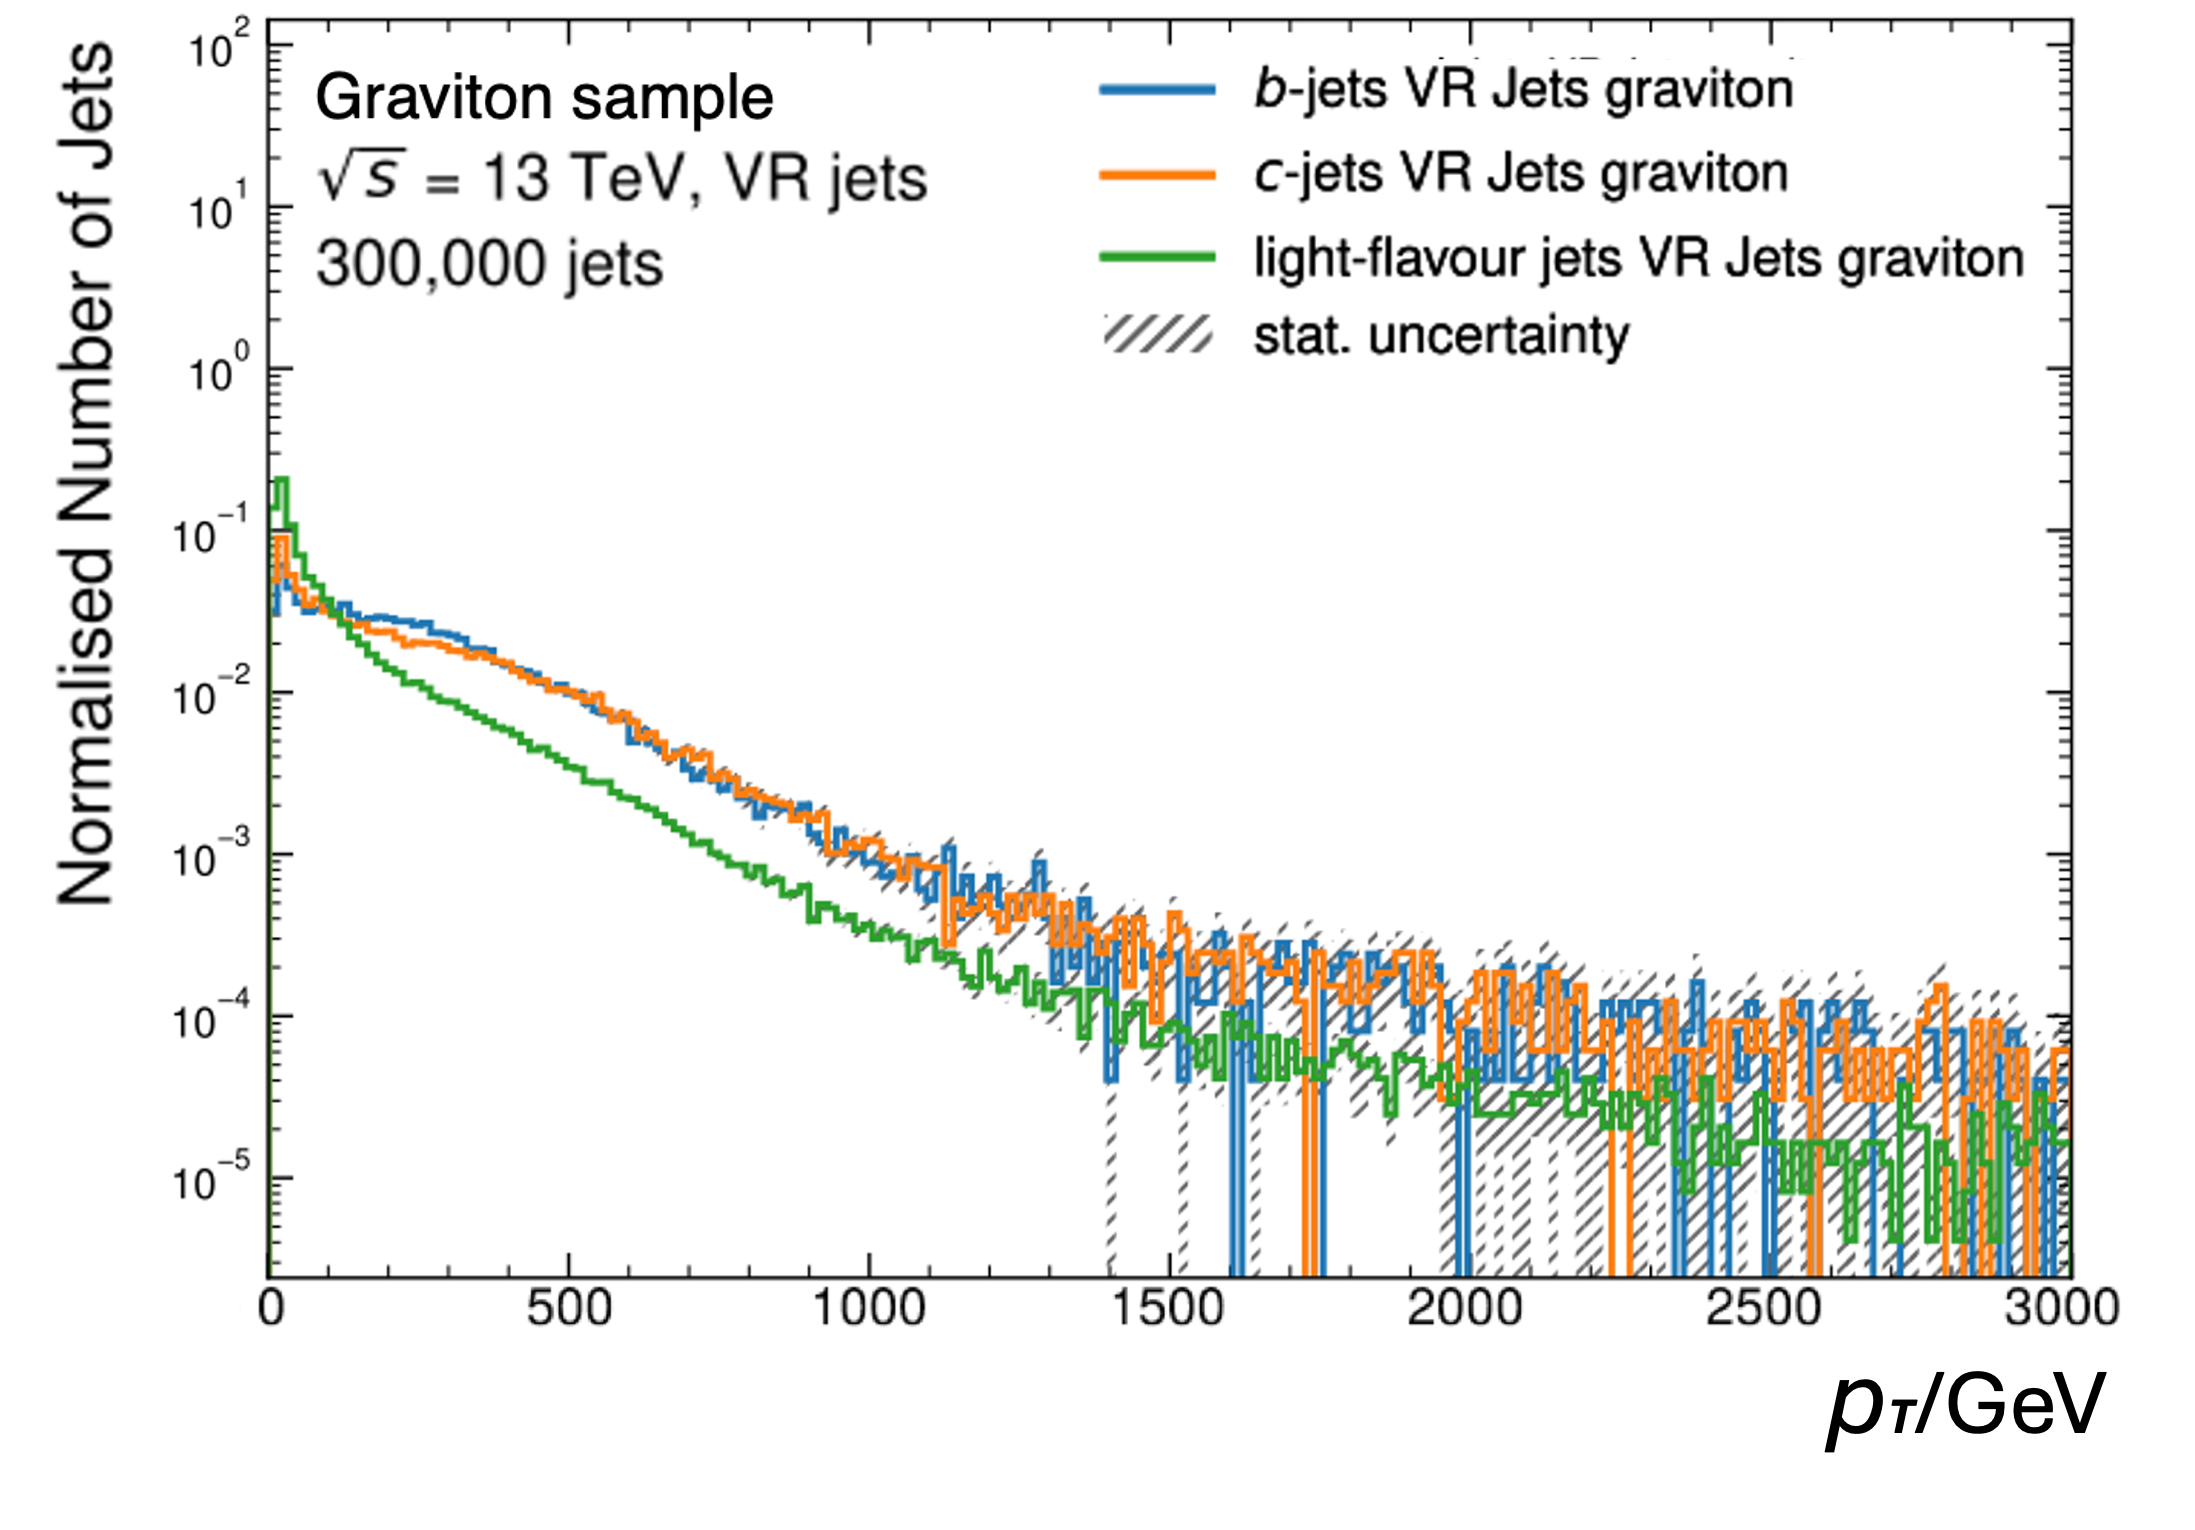
\includegraphics[width=0.48\textwidth]{Images/FTAG/VRDips/JetDist/grpt.png}
      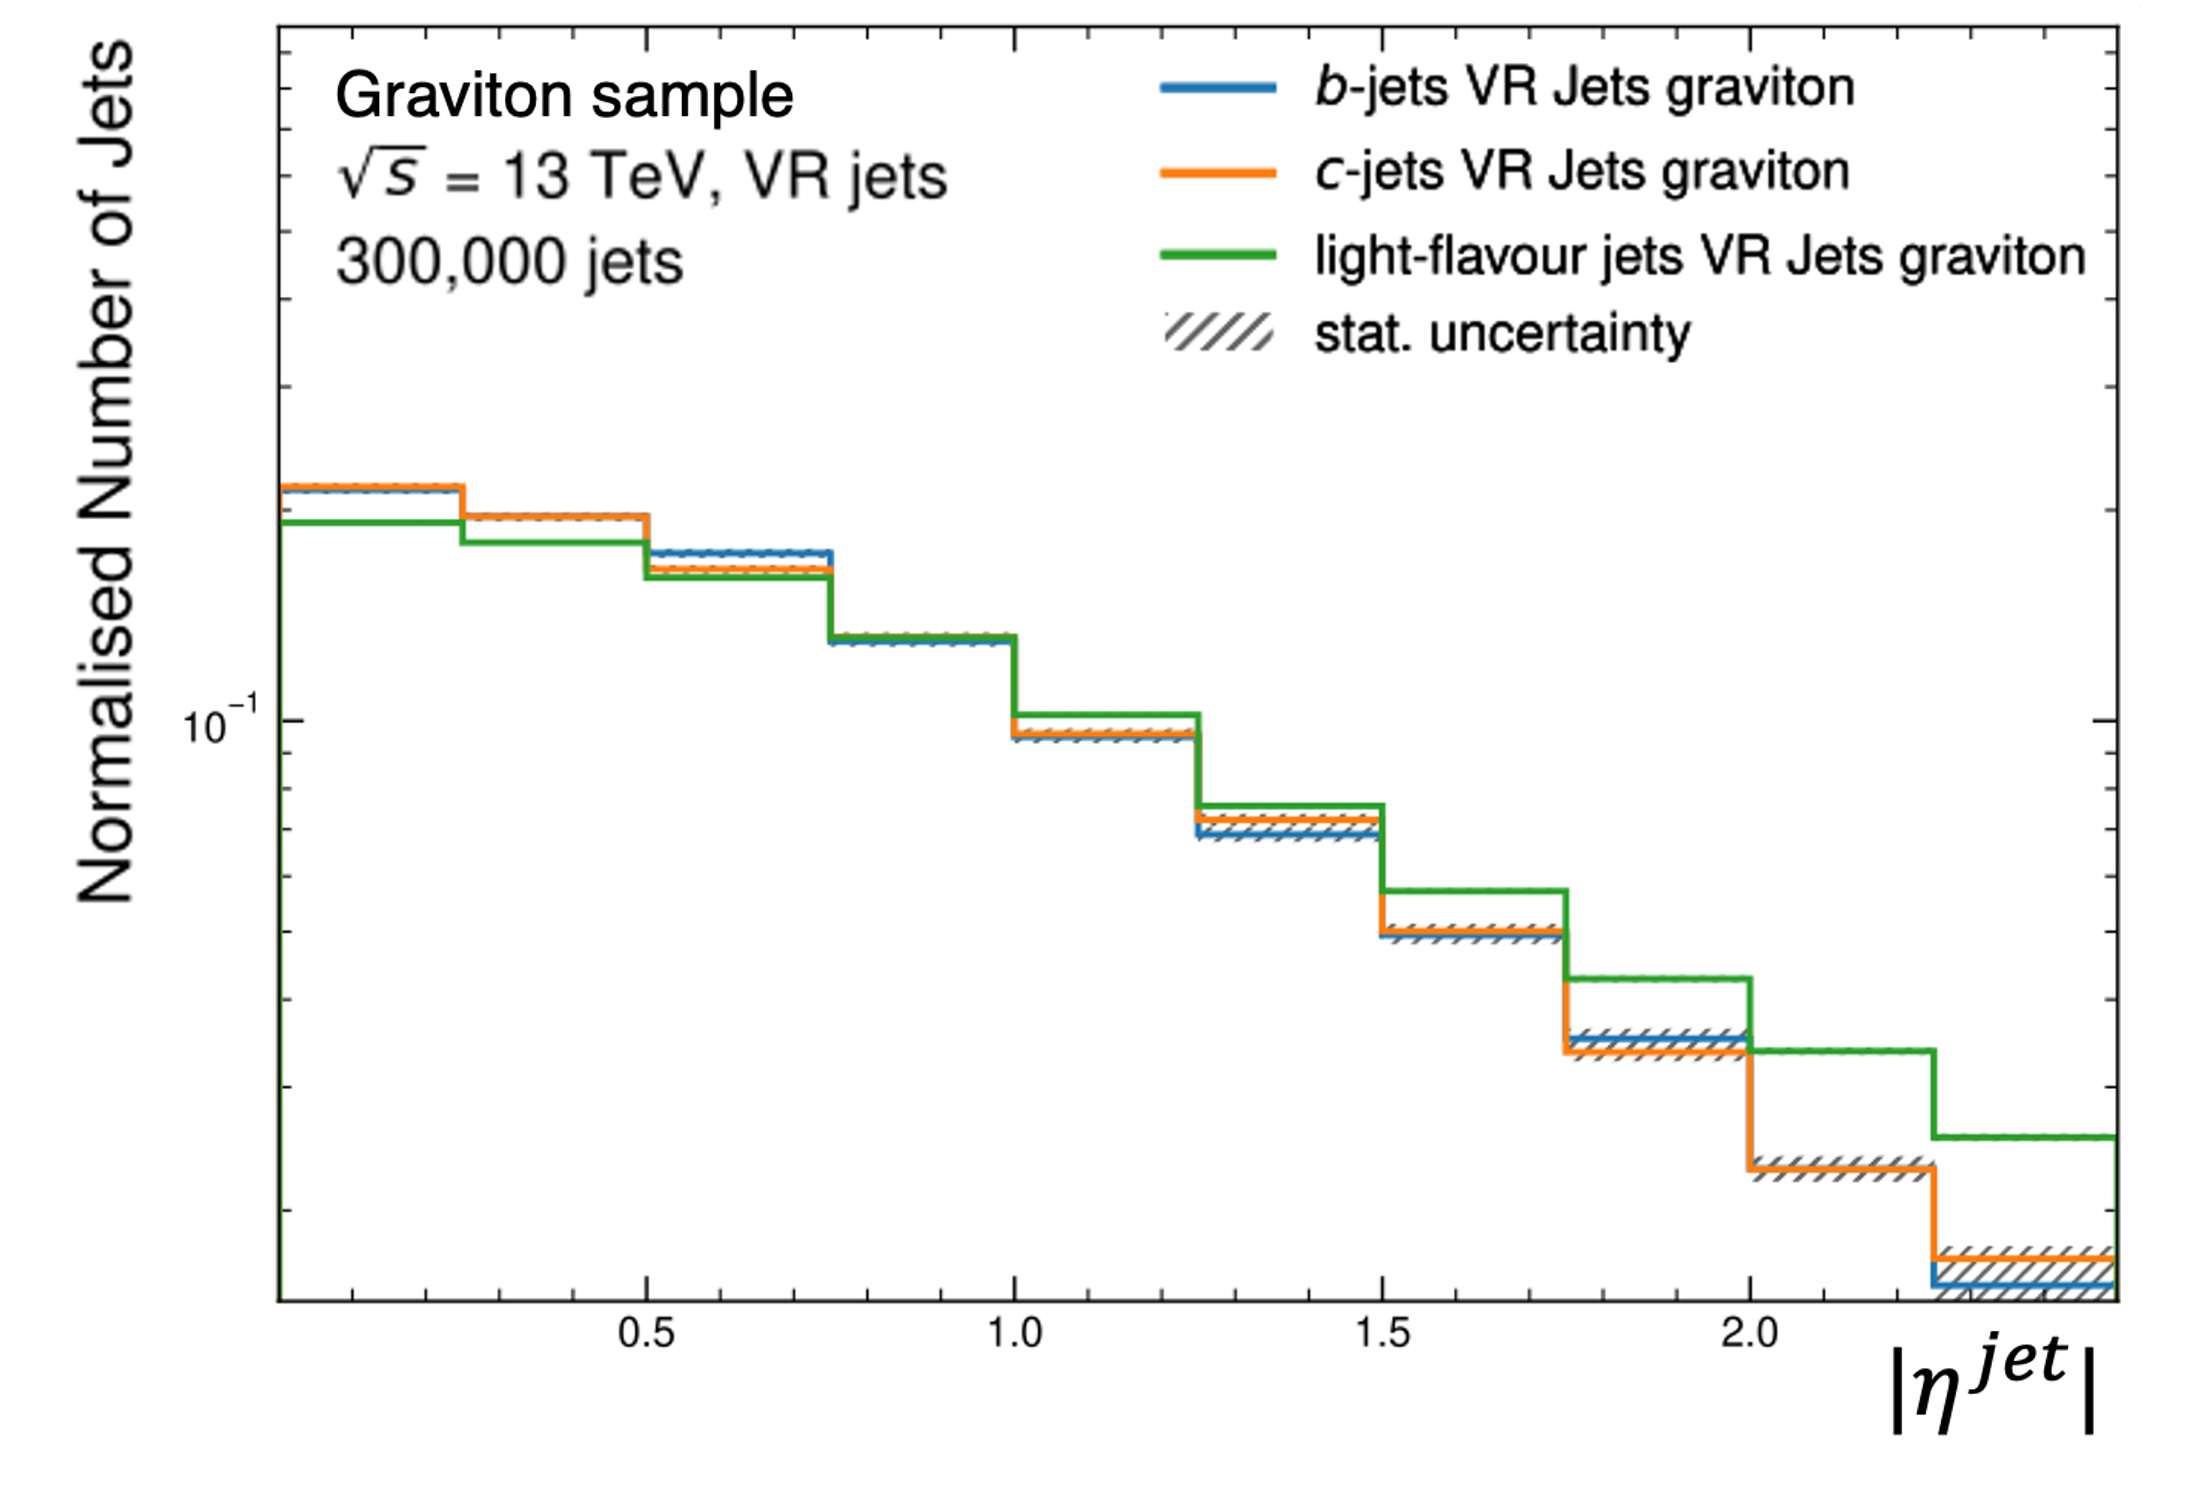
\includegraphics[width=0.48\textwidth]{Images/FTAG/VRDips/JetDist/greta.png}
      \caption{Graviton sample.} 
      \label{apfig:vrjetdisgr}
  \end{subfigure}
  \caption{Distributions for the \gls{vr}-jet training of jets $p_T$ (left) and $|\eta|$ (right) for the hybrid combined process (top row) made from the three bottom processes, in the order $t\bar{t}$, $Z'$, and the graviton.}
  \label{apfig:vrjetdist}
\end{figure} 

\section{DL1d with Variable Radius Jets}\label{ap-DL1dVR}
This section presents some plots on the VR-training of DL1d. Figure \ref{apfig:DL1dVRscanf} displays some flavour fractions scans for the $b$-tagging and $c$-tagging. 

\begin{figure}[h!]
  \centering
  \begin{subfigure}[b]{\textwidth}
      \centering
      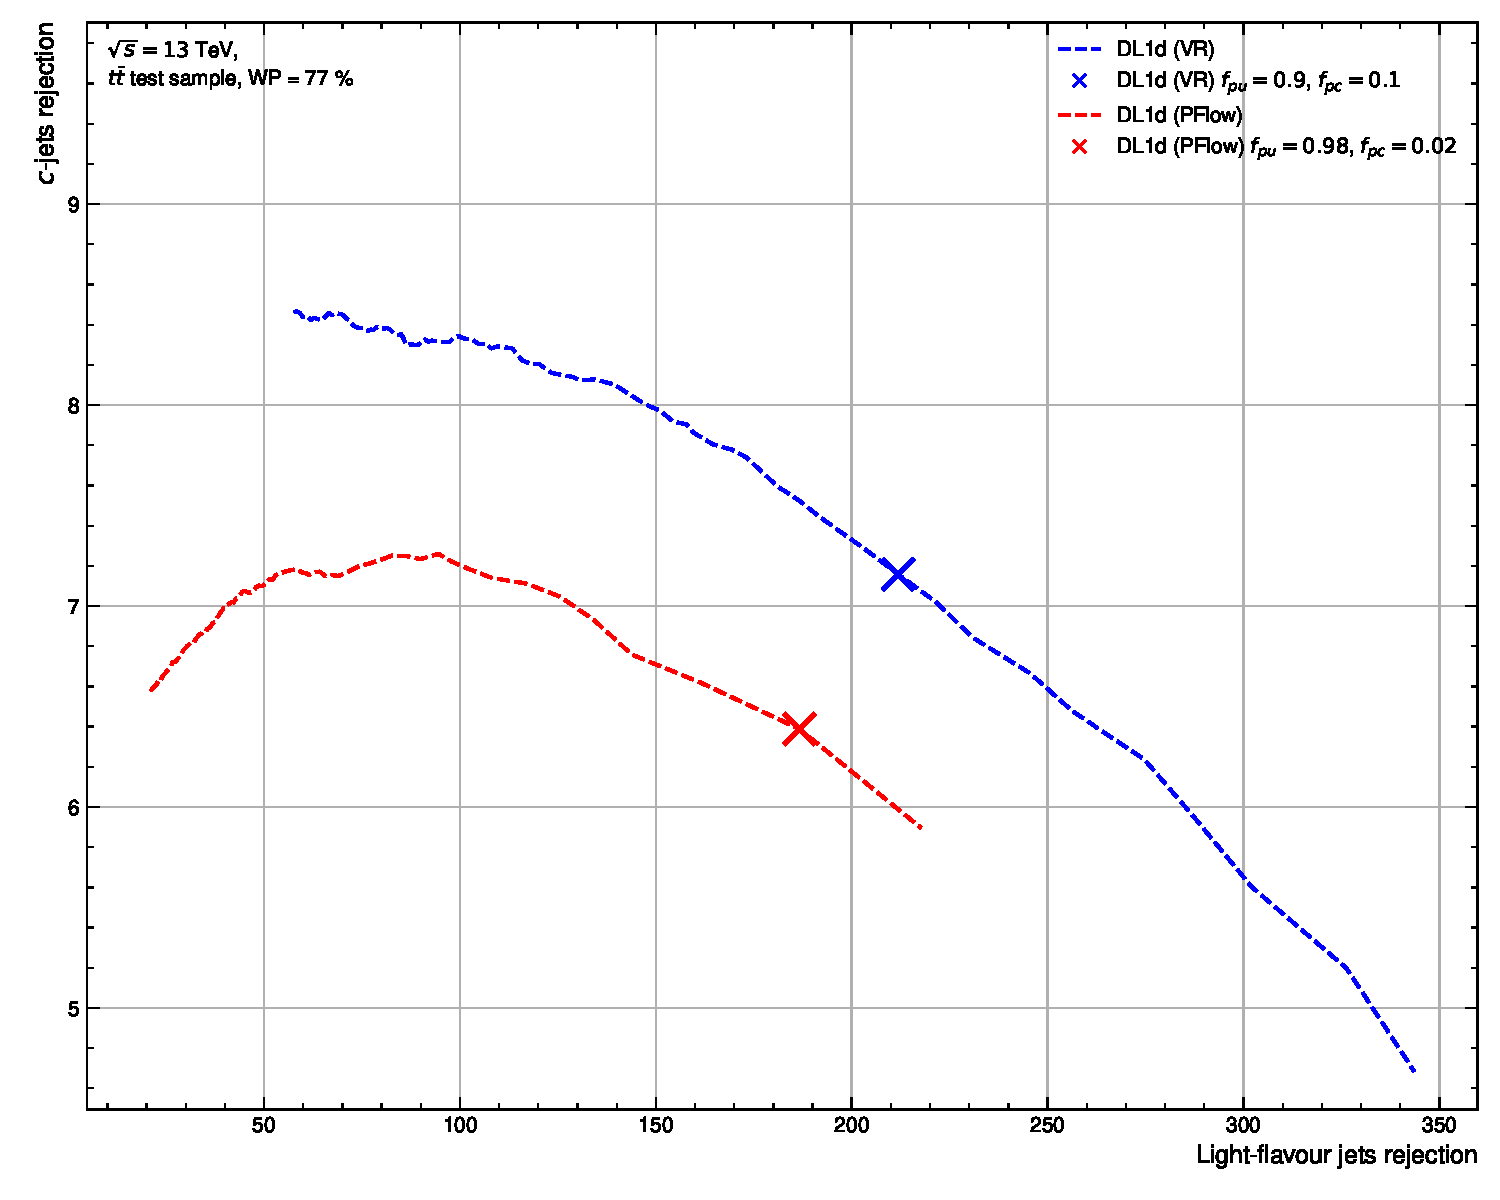
\includegraphics[width=0.32\textwidth]{Images/FTAG/VRDL1d/scansfraction/thesis_plot_frac/contour_fraction_ttbar_200.pdf}
      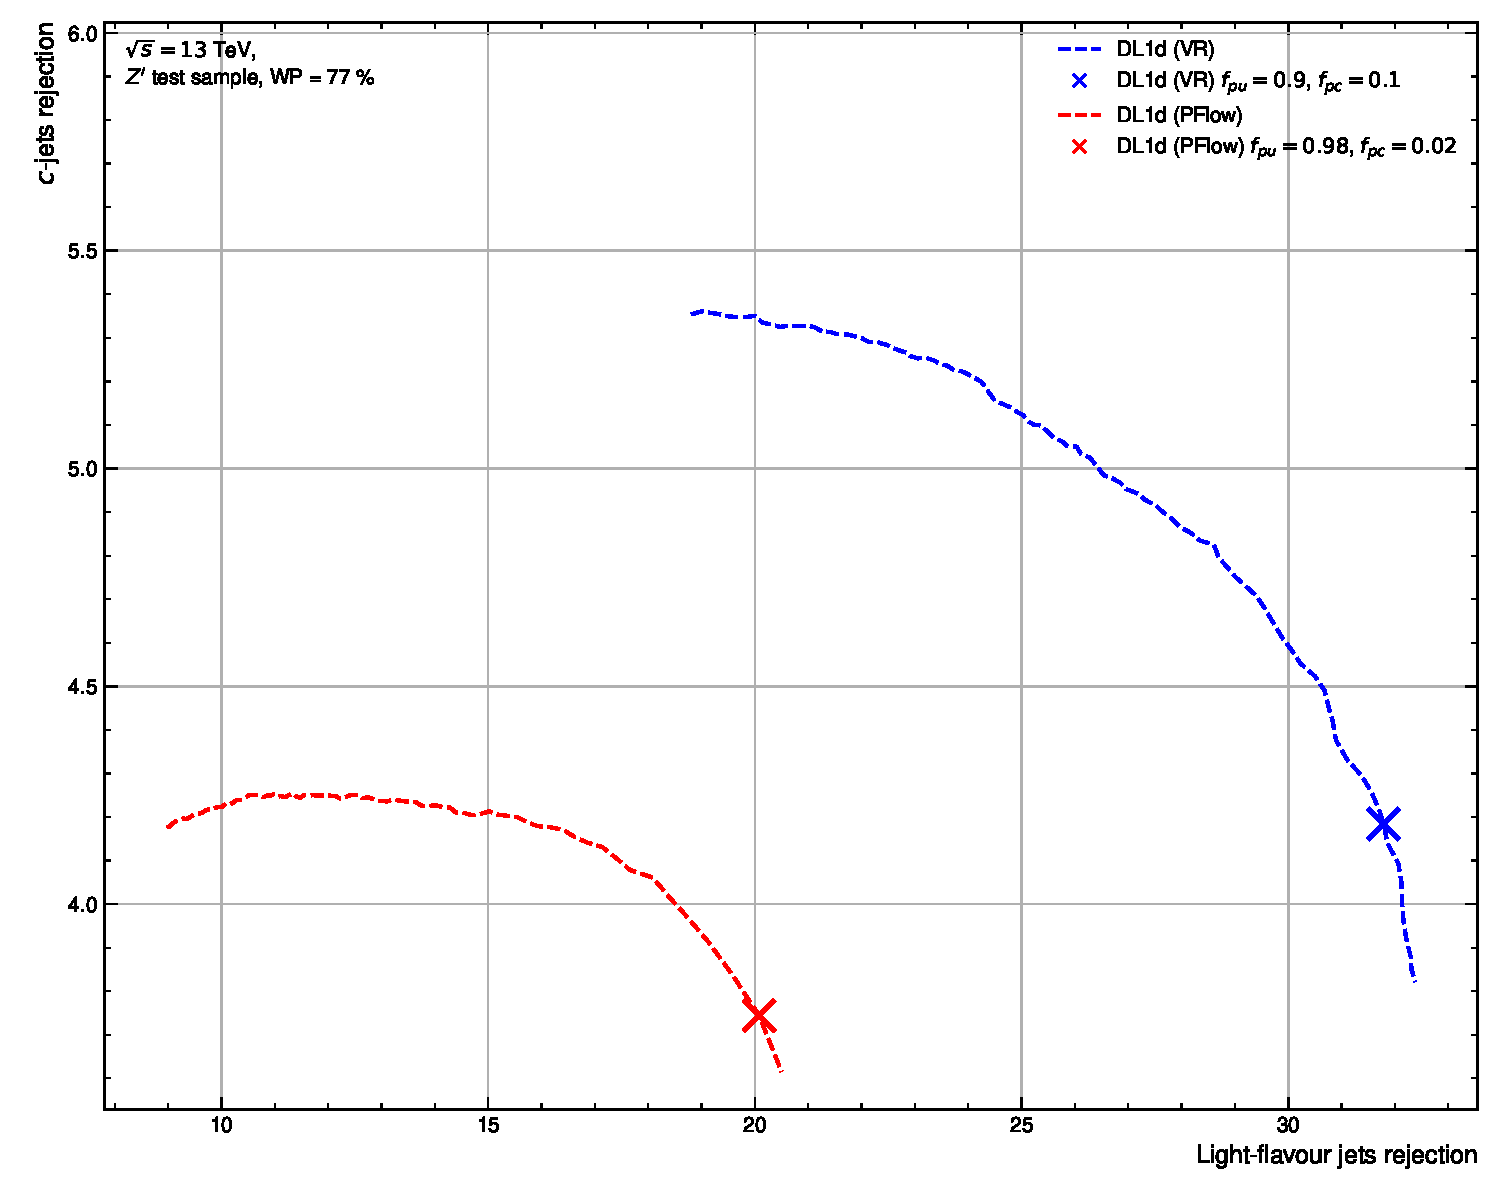
\includegraphics[width=0.32\textwidth]{Images/FTAG/VRDL1d/scansfraction/thesis_plot_frac/contour_fraction_zpext_200.pdf}
      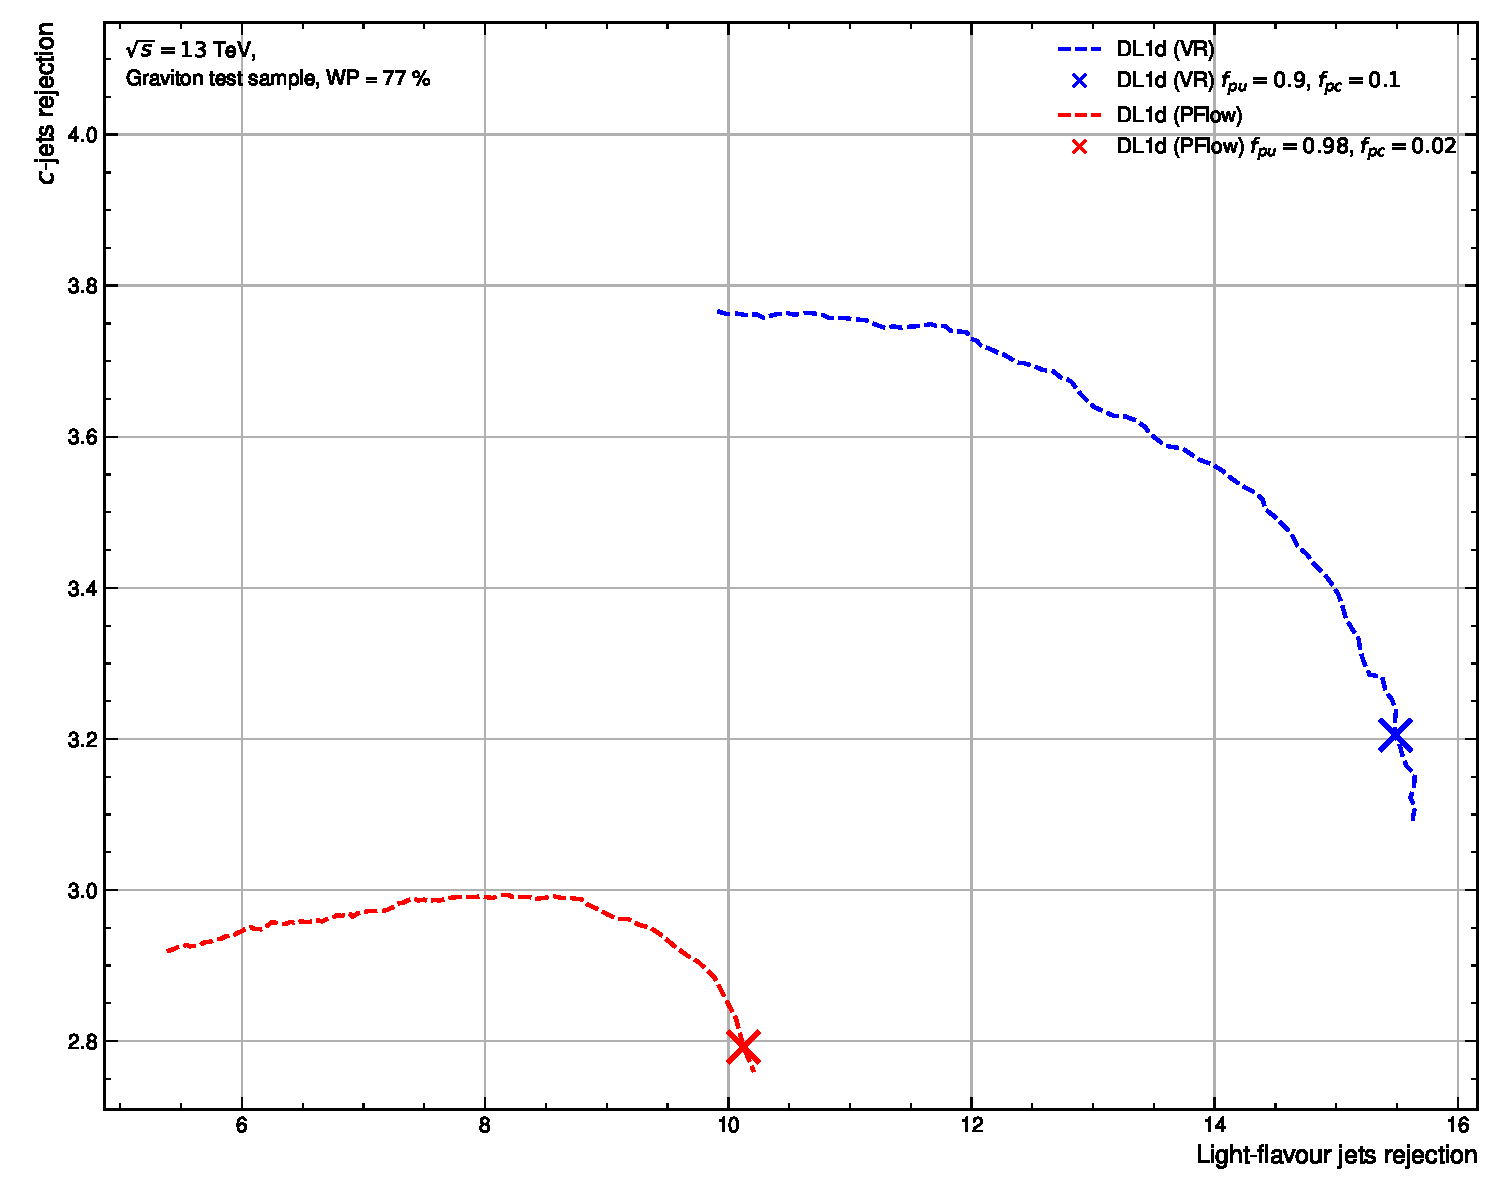
\includegraphics[width=0.32\textwidth]{Images/FTAG/VRDL1d/scansfraction/thesis_plot_frac/contour_fraction_graviton_200.pdf}
      \caption{Flavour fraction $f_c^b$ for $b$-tagging scans.} 
      \label{fig:DL1dVRscanfb}
  \end{subfigure}\\
  \begin{subfigure}[b]{\textwidth}
    \centering % UNreadable: increase font size
    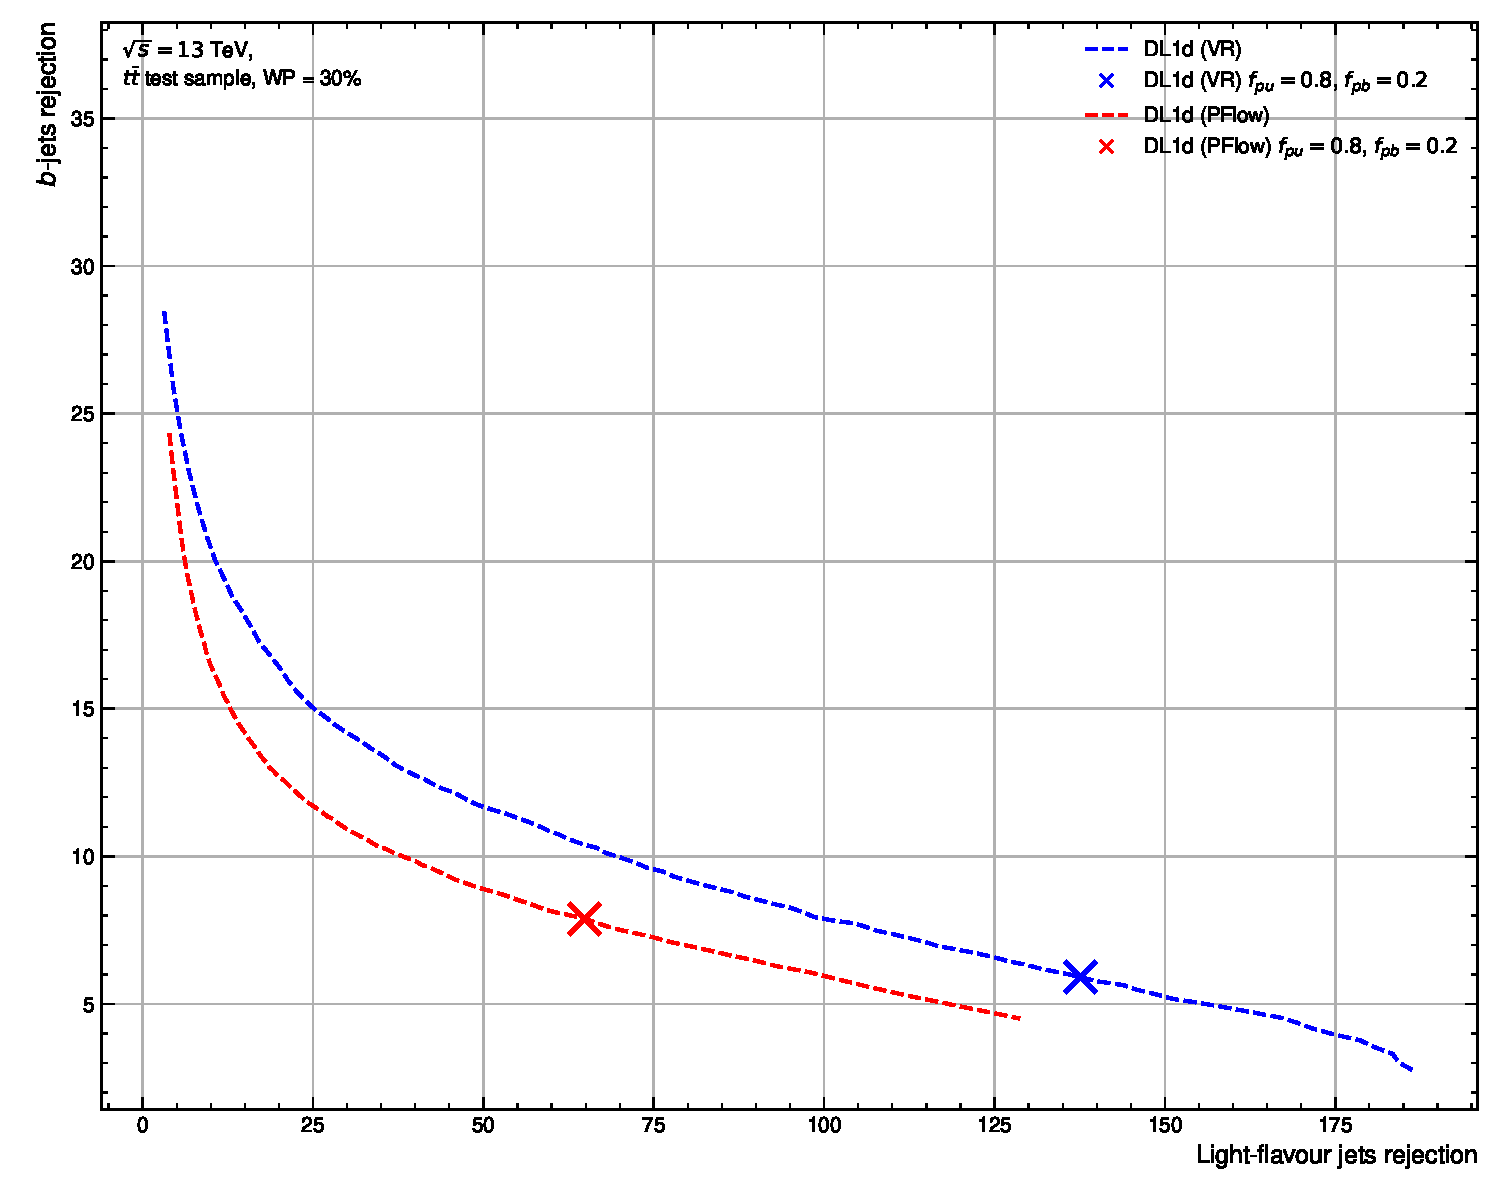
\includegraphics[width=0.32\textwidth]{Images/FTAG/VRDL1d/scansfraction/thesis_plot_frac_c/contour_fraction_ttbar_2000.pdf}
    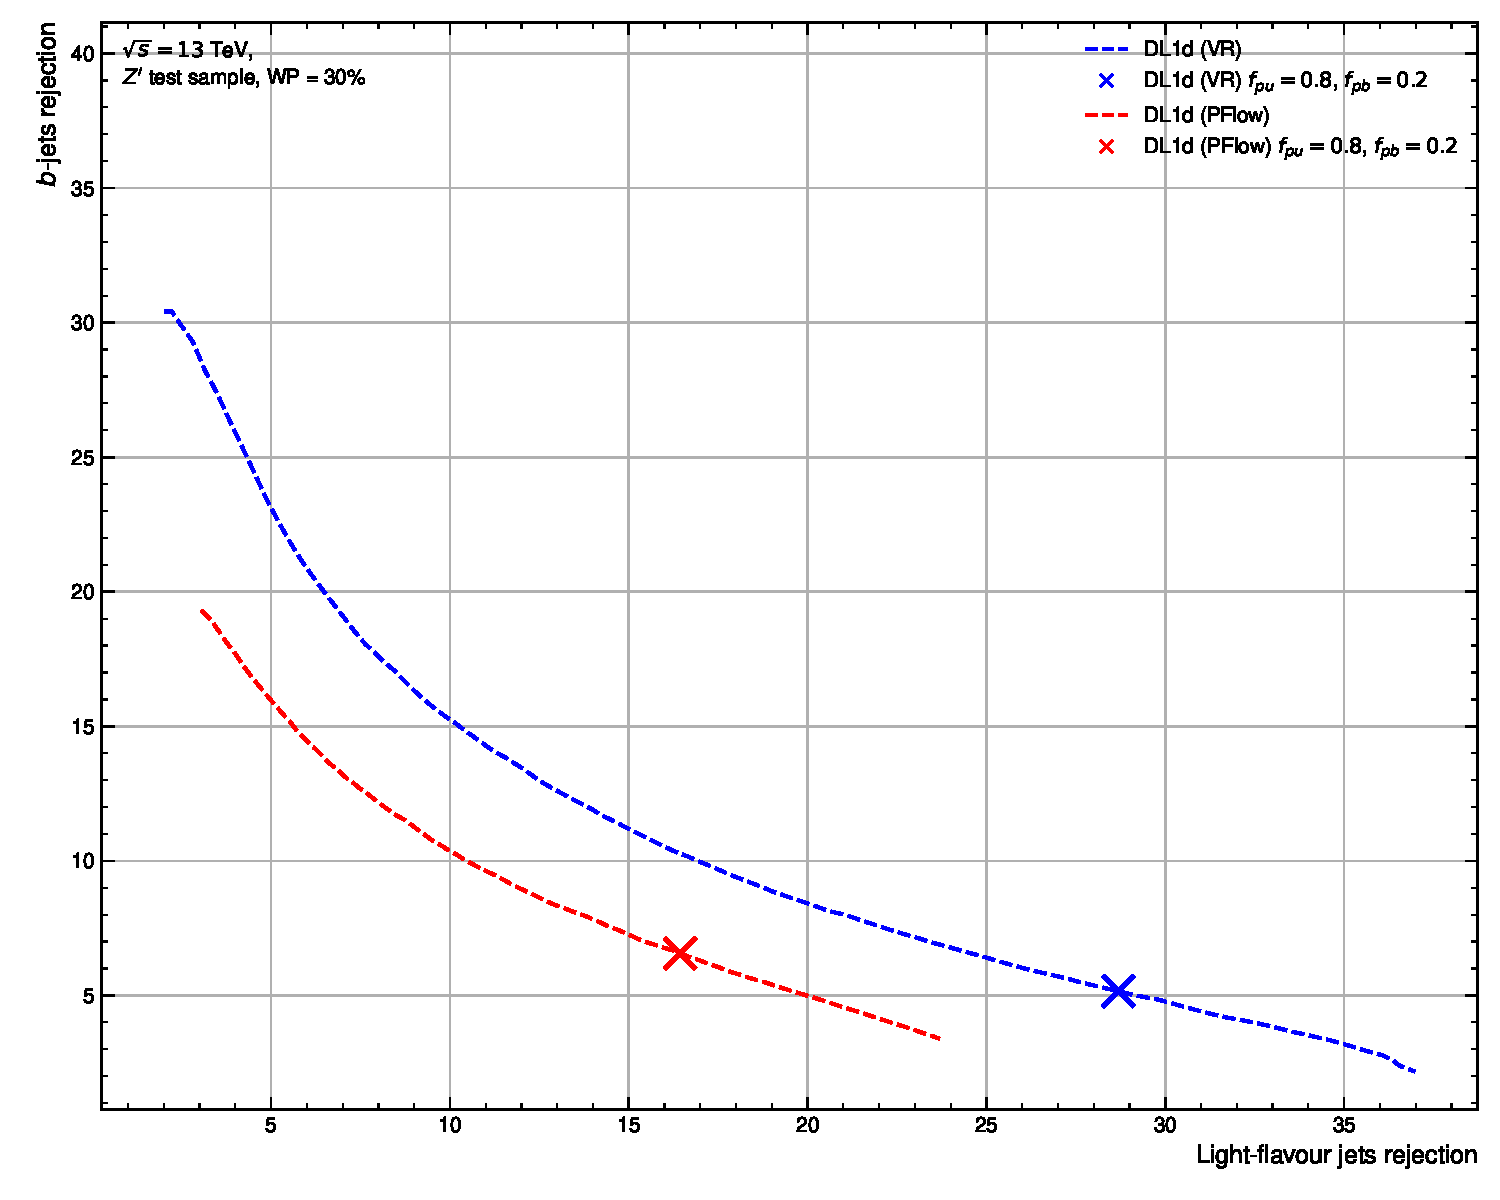
\includegraphics[width=0.32\textwidth]{Images/FTAG/VRDL1d/scansfraction/thesis_plot_frac_c/contour_fraction_zpext_2000.pdf}
    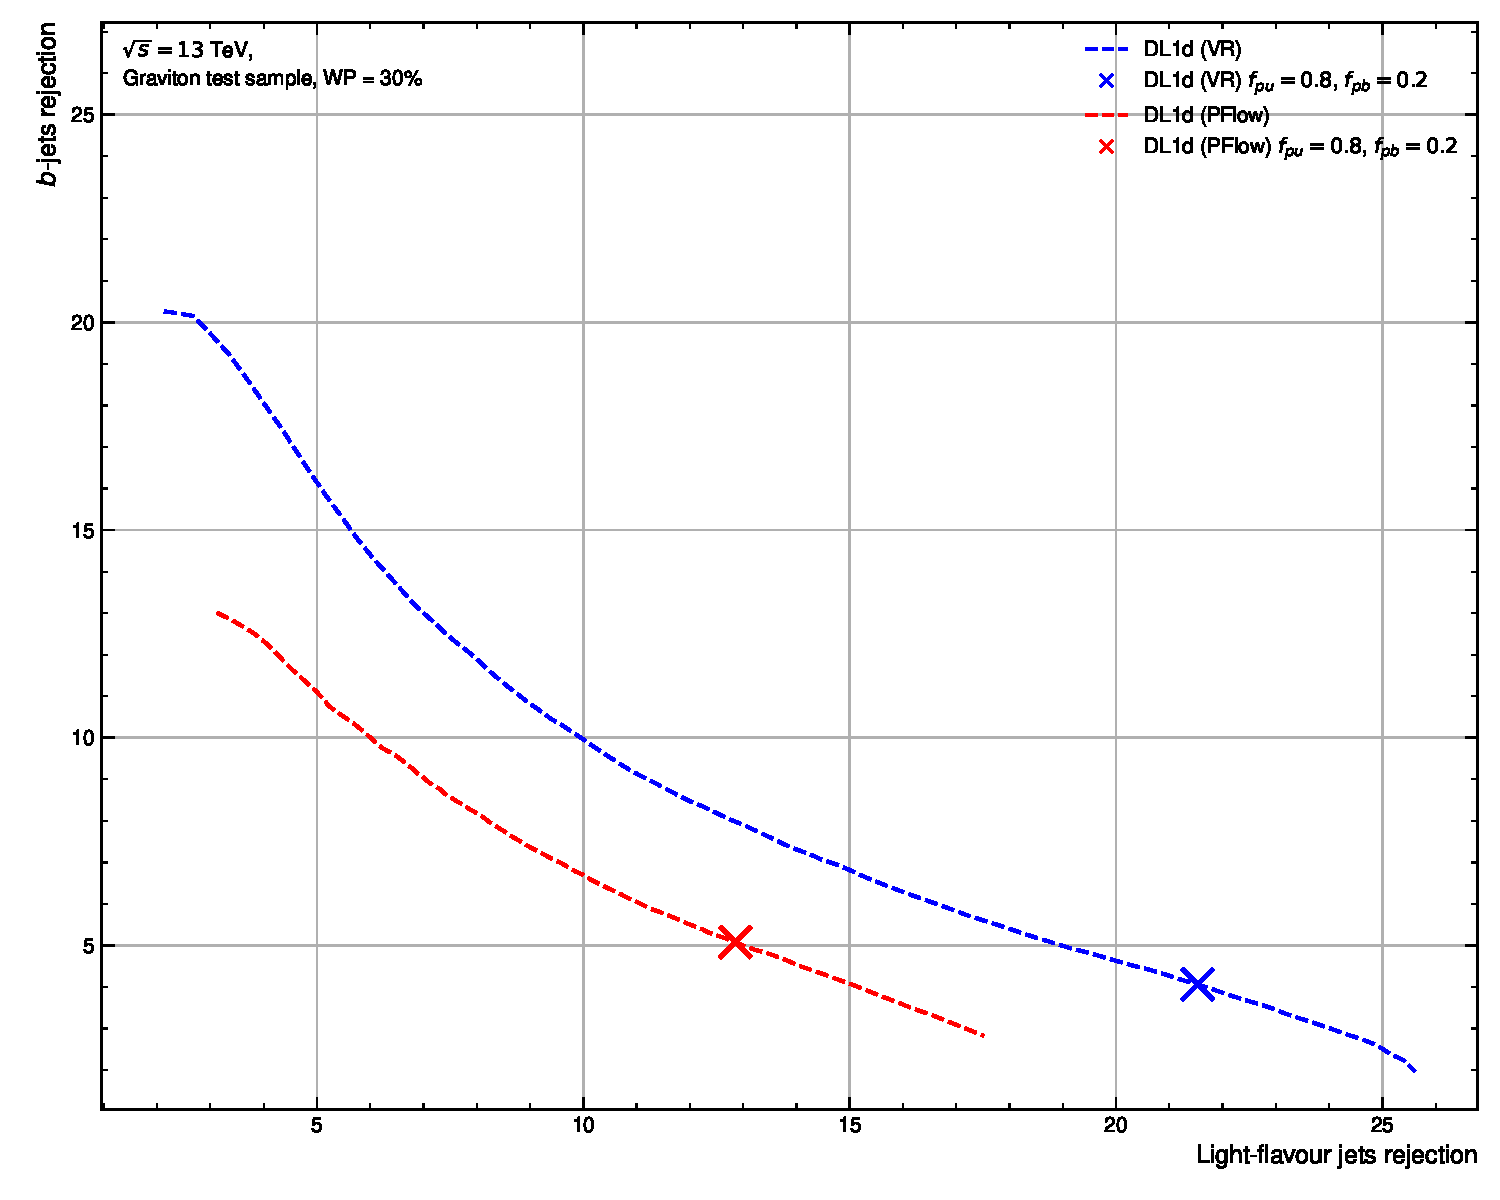
\includegraphics[width=0.32\textwidth]{Images/FTAG/VRDL1d/scansfraction/thesis_plot_frac_c/contour_fraction_graviton_2000.pdf}
    \caption{Flavour fraction $f_b^c$ for $c$-tagging scans.} 
    \label{fig:DL1dVRscanfc}
\end{subfigure}
  \caption{The flavour fractions scans of the VR- and PFlow-trained DL1d model in blue and red respectively: left is $t\bar{t}$, centre $Z'$, and right the graviton test samples. The chosen values are marked on the curves, displaying on the $y$-axis the $c$-rejection ($b$-rejection) for $b$-tagging ($c$-tagging) vs the light-rejection on the $x$ axis at a fixed working point of 77\% (33\%). Increasing $f_c$ or $f_b$ shifts the marker upwards along the curves. }
  \label{apfig:DL1dVRscanf}
\end{figure} 

\section{GN2 public plots}
A comparison of the global performance of this \gls{gn2} model to the \gls{dl1d} and \gls{gn1} models is displayed in the $b$- and $c$-tagging \gls{roc} curves of Figures \ref{fig:GN2rocb} and \ref{fig:GN2rocc}. These results are taken from Ref \cite{ATL-PLOT-FTAG-2023-01}, for which the \gls{dl1d} model was retrained on the same dataset as \gls{gn2}, and the \gls{dl1r} and \gls{gn1} models are taken from Chapter \ref{chap-GN1}. \gls{gn2} delivers yet another significant boost to performance, drasticaly surpassing the \gls{gn1} rejections at all efficiencies considered. The largest improvement is again obtained at lower $b$-jet efficiencies. Compared to \gls{gn1}, \gls{gn2} delivers $\times 1.5$ ($\times 1.7$) the $c$-rejection (light-rejection) on $t\bar{t}$ at the 70\% $b$-tagging \gls{wp} and $\times 1.75$ ($\times 1.2$) on $Z'$ at 30\% \gls{wp}. With respect to \gls{dl1d}, the gains in $c$-rejection (light-rejection) are respectively close to $\times 3$ ($\times 2$) for $t\bar{t}$ and $\times 3.4$ ($\times 4$) on $Z'$. 

\begin{center}
    \vspace{-1.cm}
    \begin{figure}[h!]
    \centerline{
    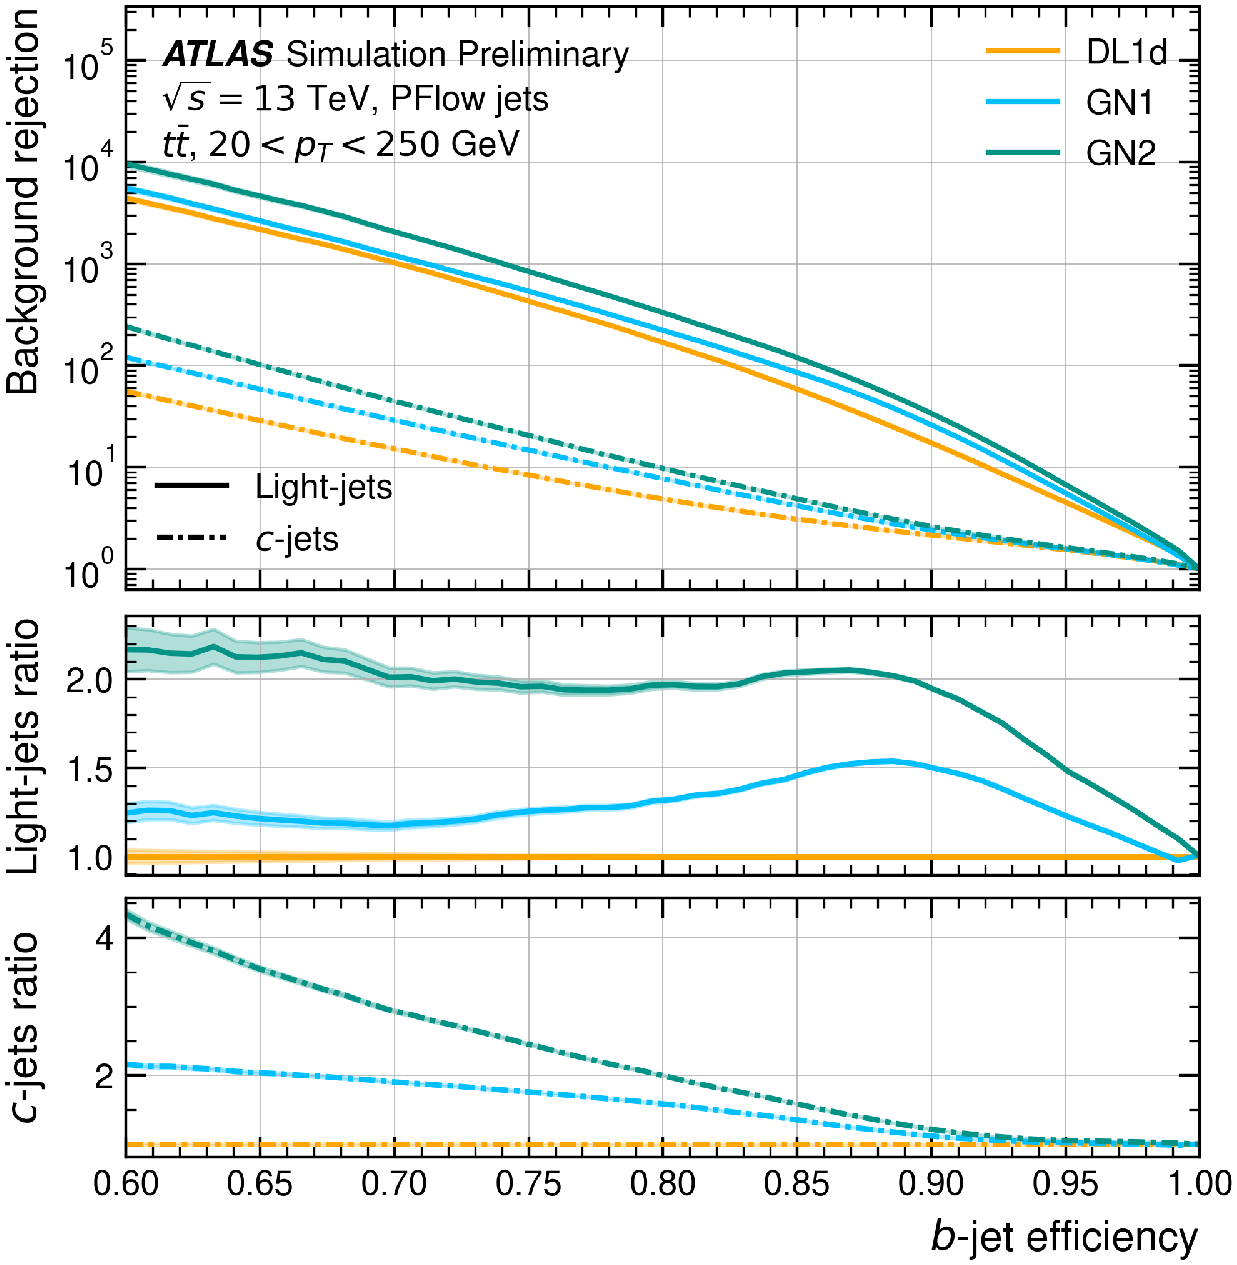
\includegraphics[width=0.48\textwidth]{Images/FTAG/GN/GN2/ROCpublic/ttb.png}
    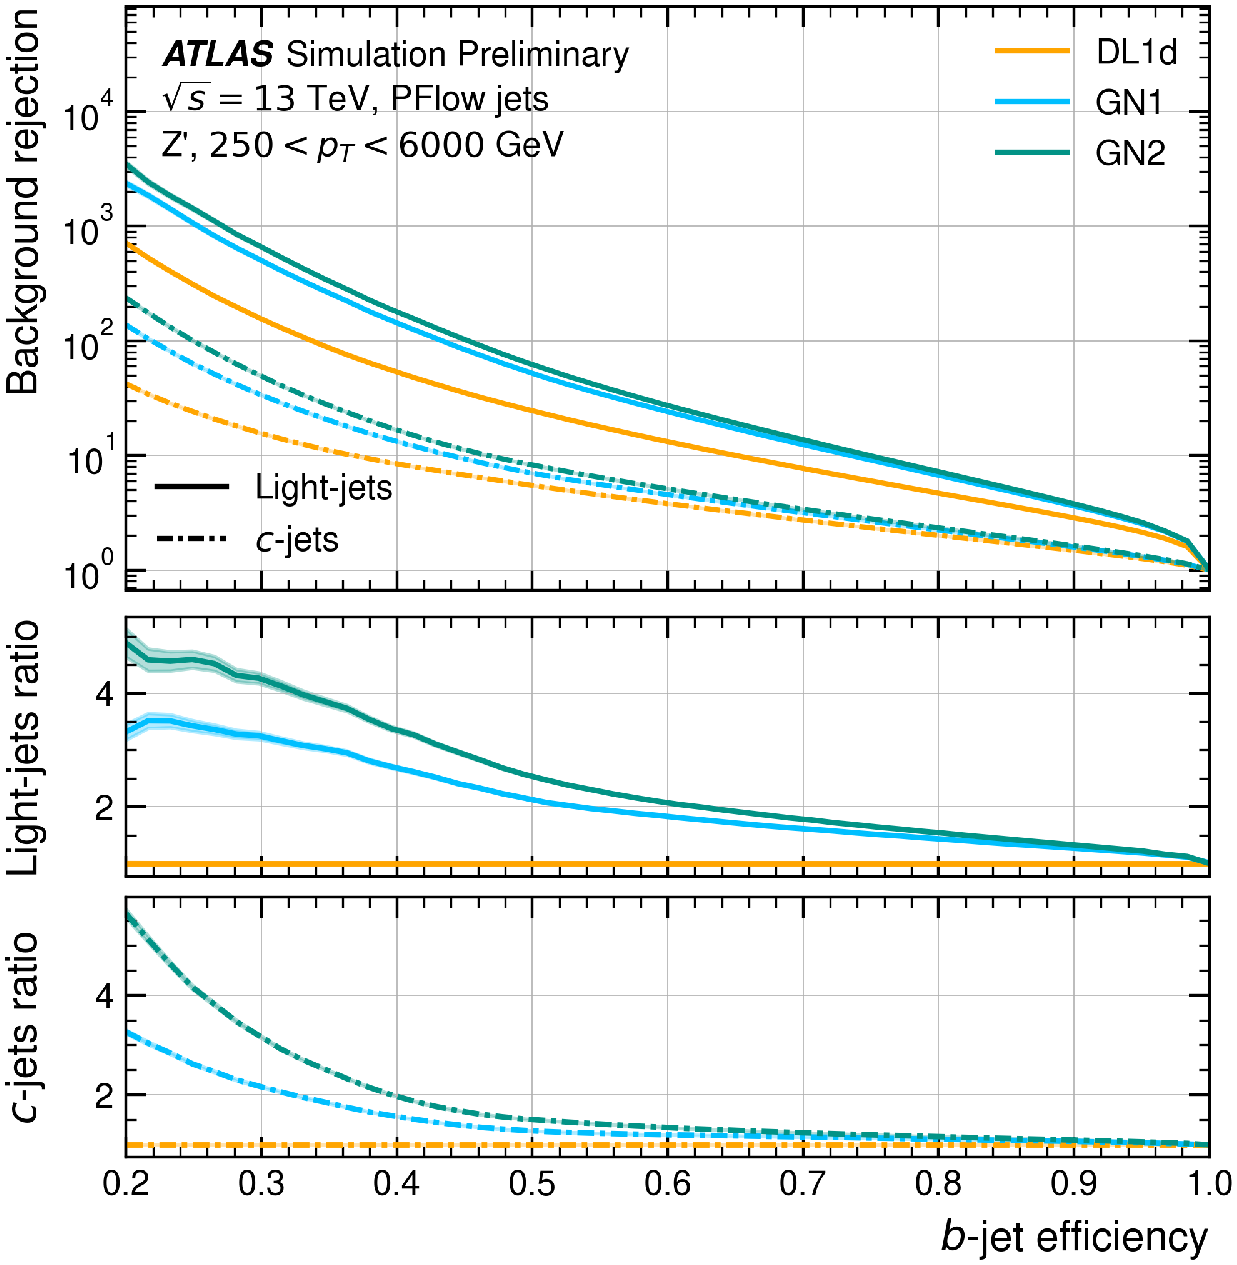
\includegraphics[width=0.48\textwidth]{Images/FTAG/GN/GN2/ROCpublic/zpb.png}
    }
    \caption{The $c$- and light-rejections as a function of the $b$-jet tagging efficiency in the $t\bar{t}$ with $20 < p_T < 250$ GeV (left) and $Z'$ with $250 < p_T < 6000$ GeV (right) test samples, from \cite{ATL-PLOT-FTAG-2023-01}. Models compared are DL1d in orange, GN1 in turquoise, and GN2 in blue. The bottom plots show the ratio with respect to the DL1d performance. Flavour fractions are set at $f^b_c = 0.018$ for DL1d, 0.05 for GN1, and 0.1 for GN2. Shaded regions represent the binominal error band.}
    \label{apfig:GN2rocb}
    \bigskip
    \centerline{
    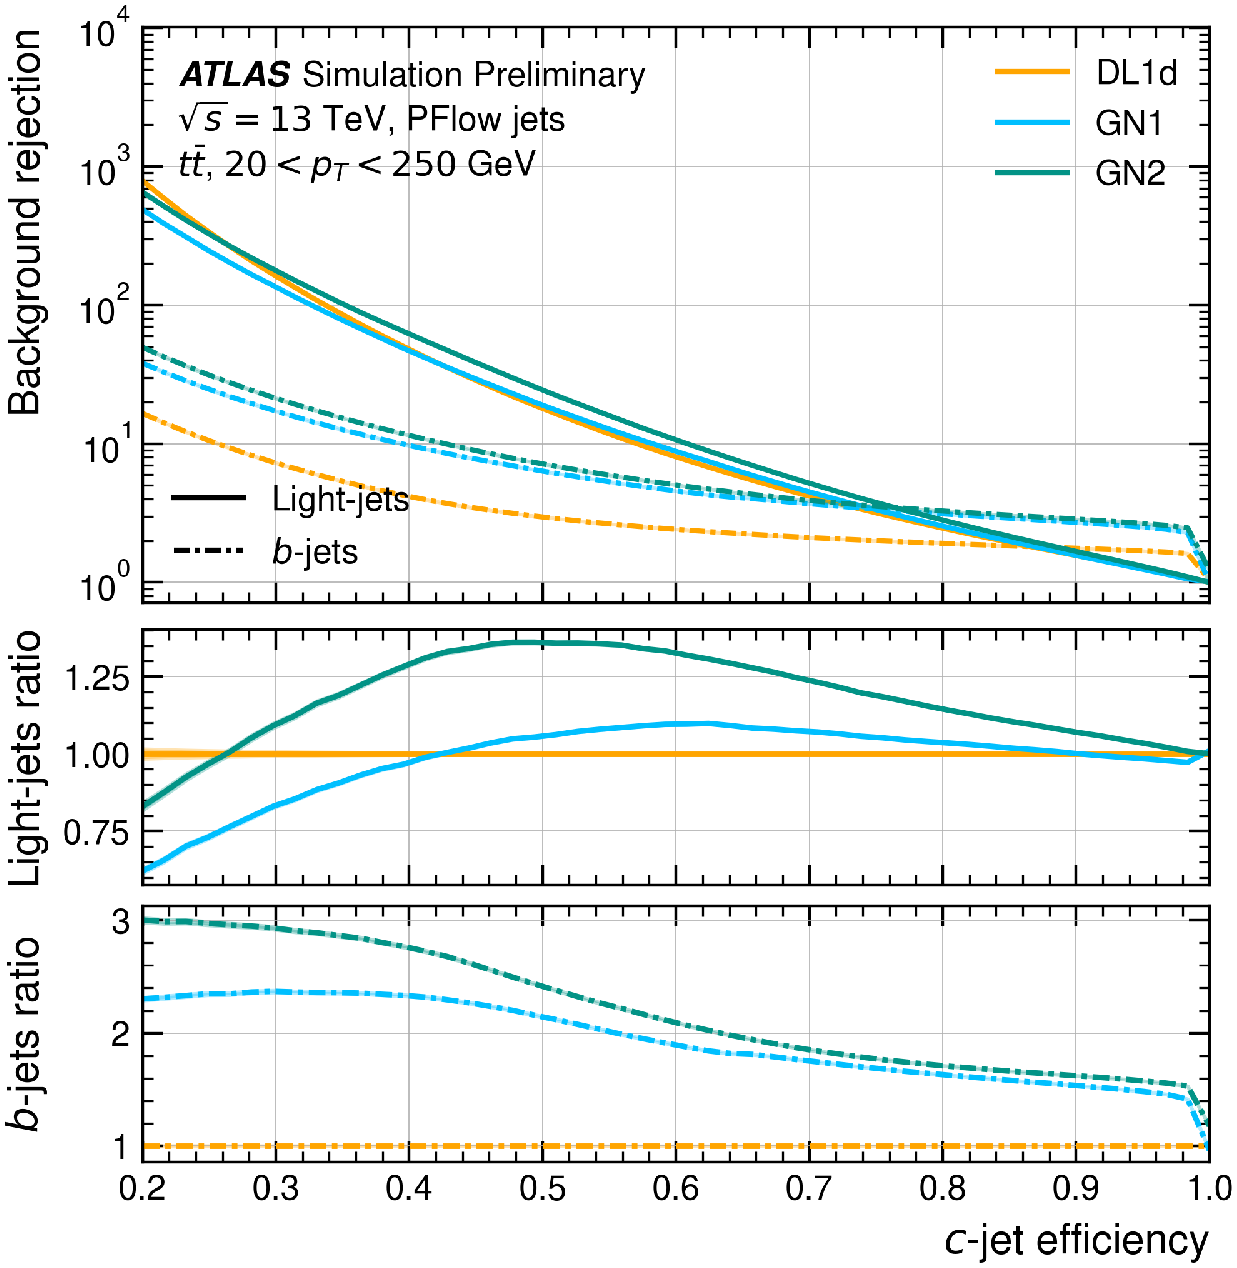
\includegraphics[width=0.48\textwidth]{Images/FTAG/GN/GN2/ROCpublic/ttc.png}
    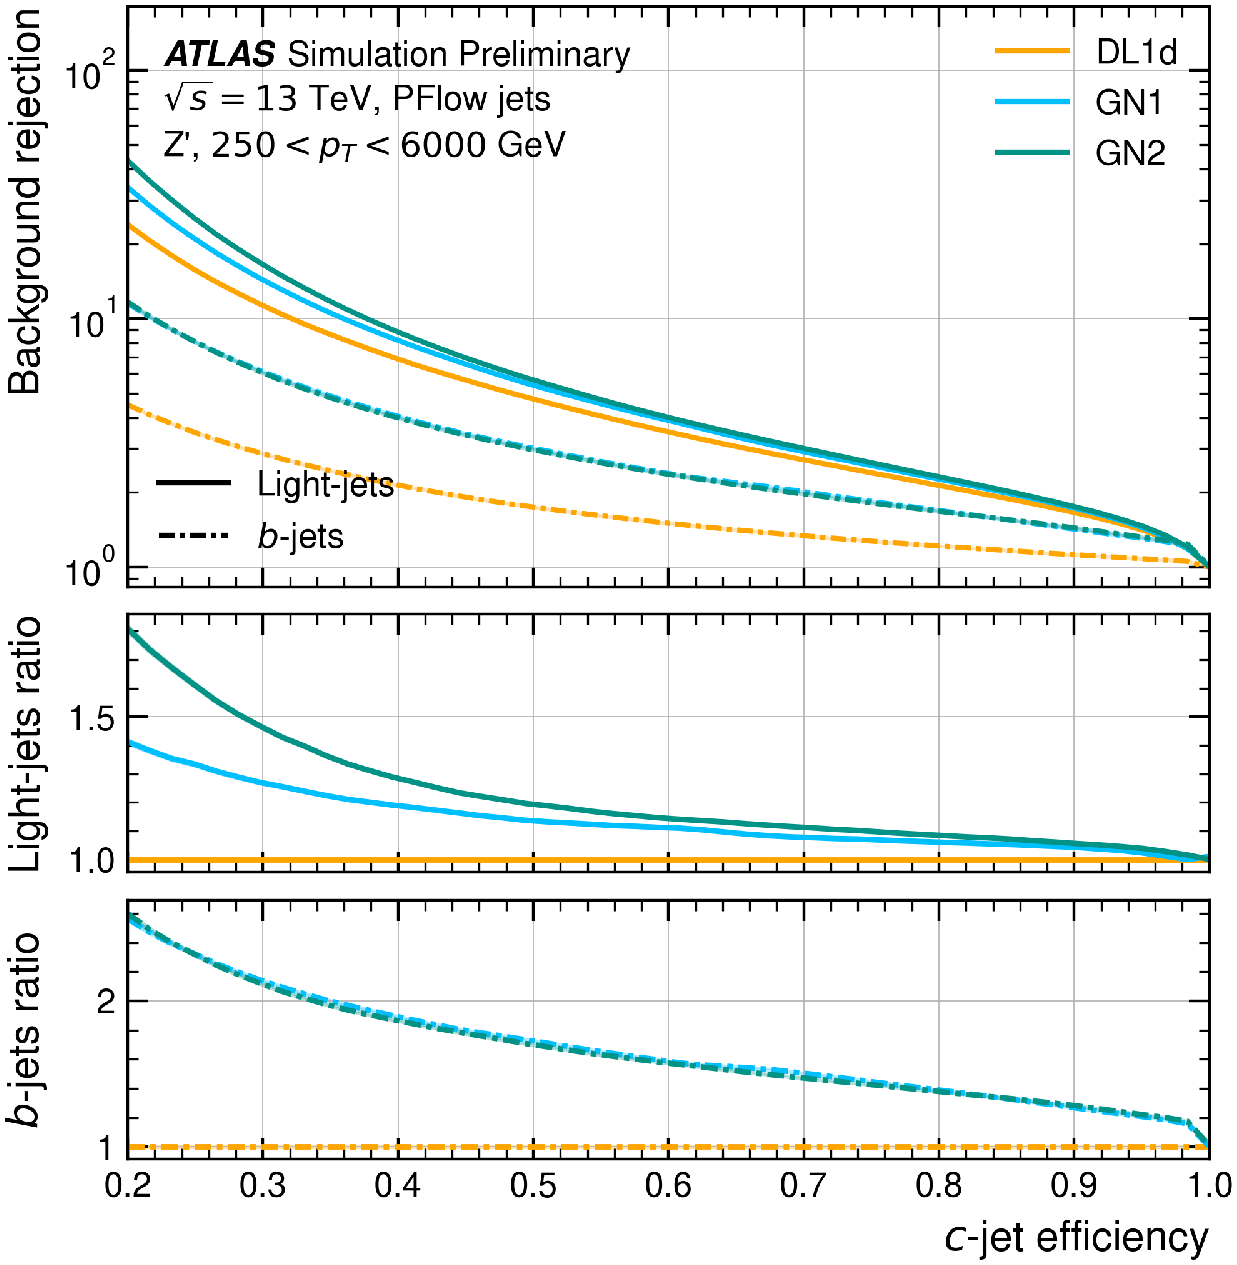
\includegraphics[width=0.48\textwidth]{Images/FTAG/GN/GN2/ROCpublic/zpc.png}
    }
    \caption{The $b$- and light-rejections as a function of the $c$-jet tagging efficiency in the $t\bar{t}$ with $20 < p_T < 250$ GeV (left) and $Z'$ with $250 < p_T < 6000$ GeV (right) test samples, from \cite{ATL-PLOT-FTAG-2023-01}. Models compared are DL1d in orange, GN1 in turquoise, and GN2 in blue. The bottom plots show the ratio with respect to the DL1d performance. Flavour fractions are set at $f^c_b = 0.2$ for all taggers. Shaded regions represent the binominal error band.}
    \label{apfig:GN2rocc}
    \end{figure}
\end{center}

Turning to $c$-tagging, a similar large performance gained is obtained by the new \gls{gnn} family over \gls{dl1d}, although the change on the $t\bar{t}$ is more impressive for the $b$-jet ratio than for light-jet. This indicates a non-optimal choice for the flavour fraction $f^c_b$, which was set at 0.2 for all models.

\section{GN2 supporting plots}\label{app-GN2sup}
This section presents more plots in support of Chapter \ref{chap-GN2}. Figure \ref{apfig:GNxptc_eff} presents the $c$-tagging efficiency per bin for an overall $c$-tagging working point of 30\% per region displayed. 

\begin{figure}[h!]
    \centering
    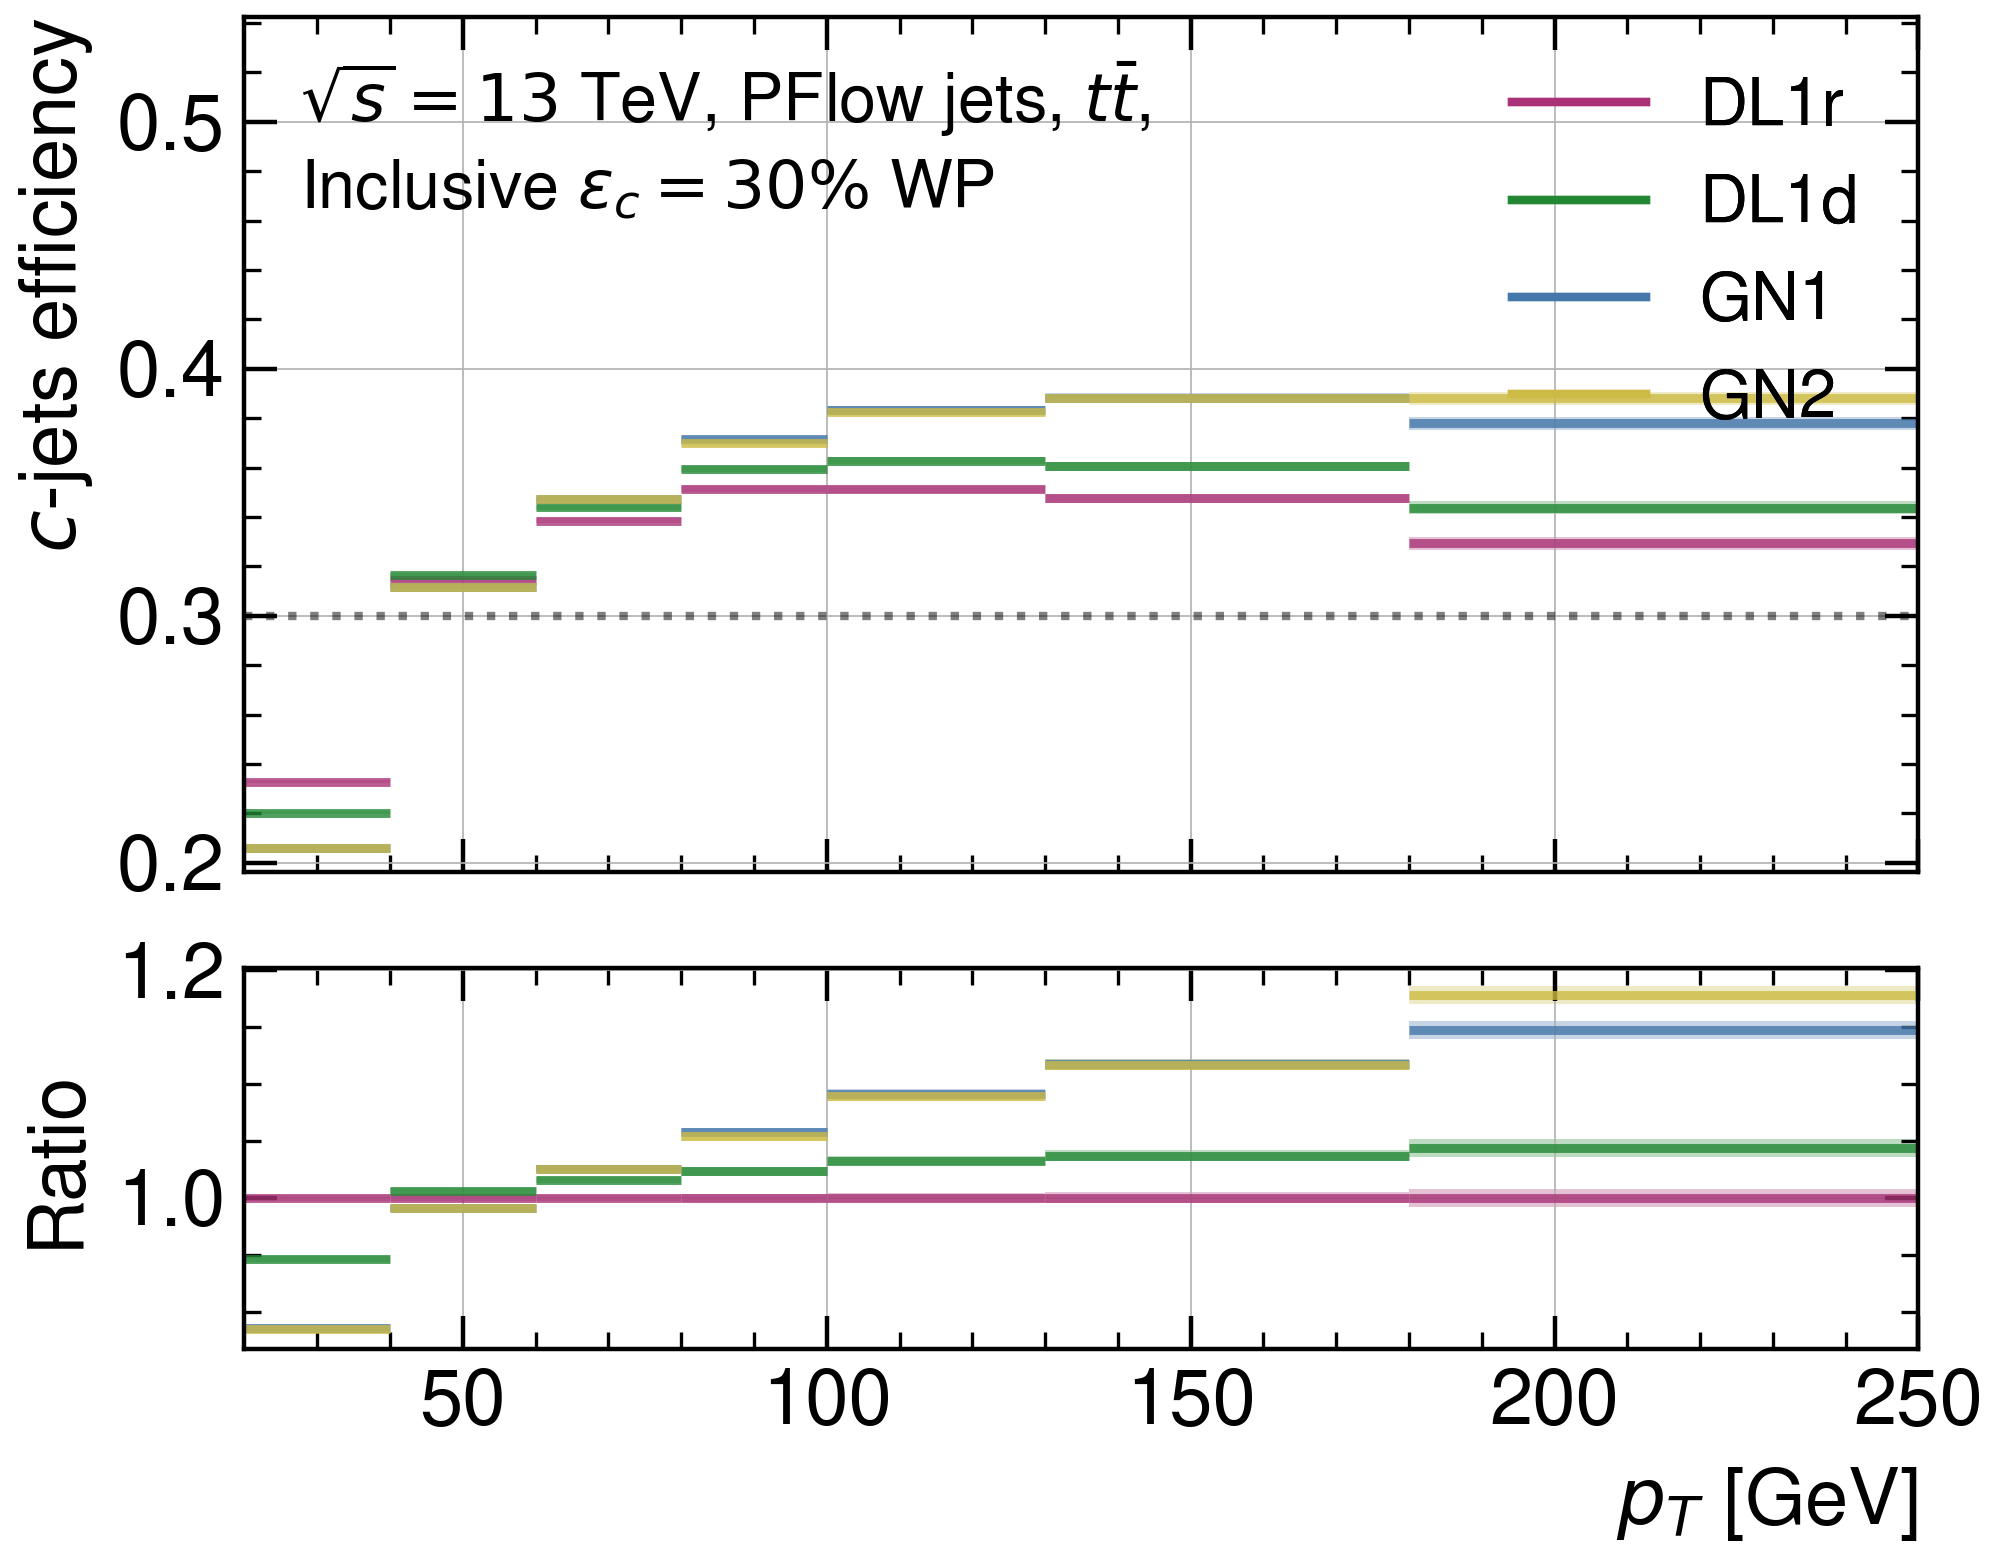
\includegraphics[width=0.48\textwidth]{Images/FTAG/GN/GN2/pt_plots/pt_ttbar_c_eff.png}
    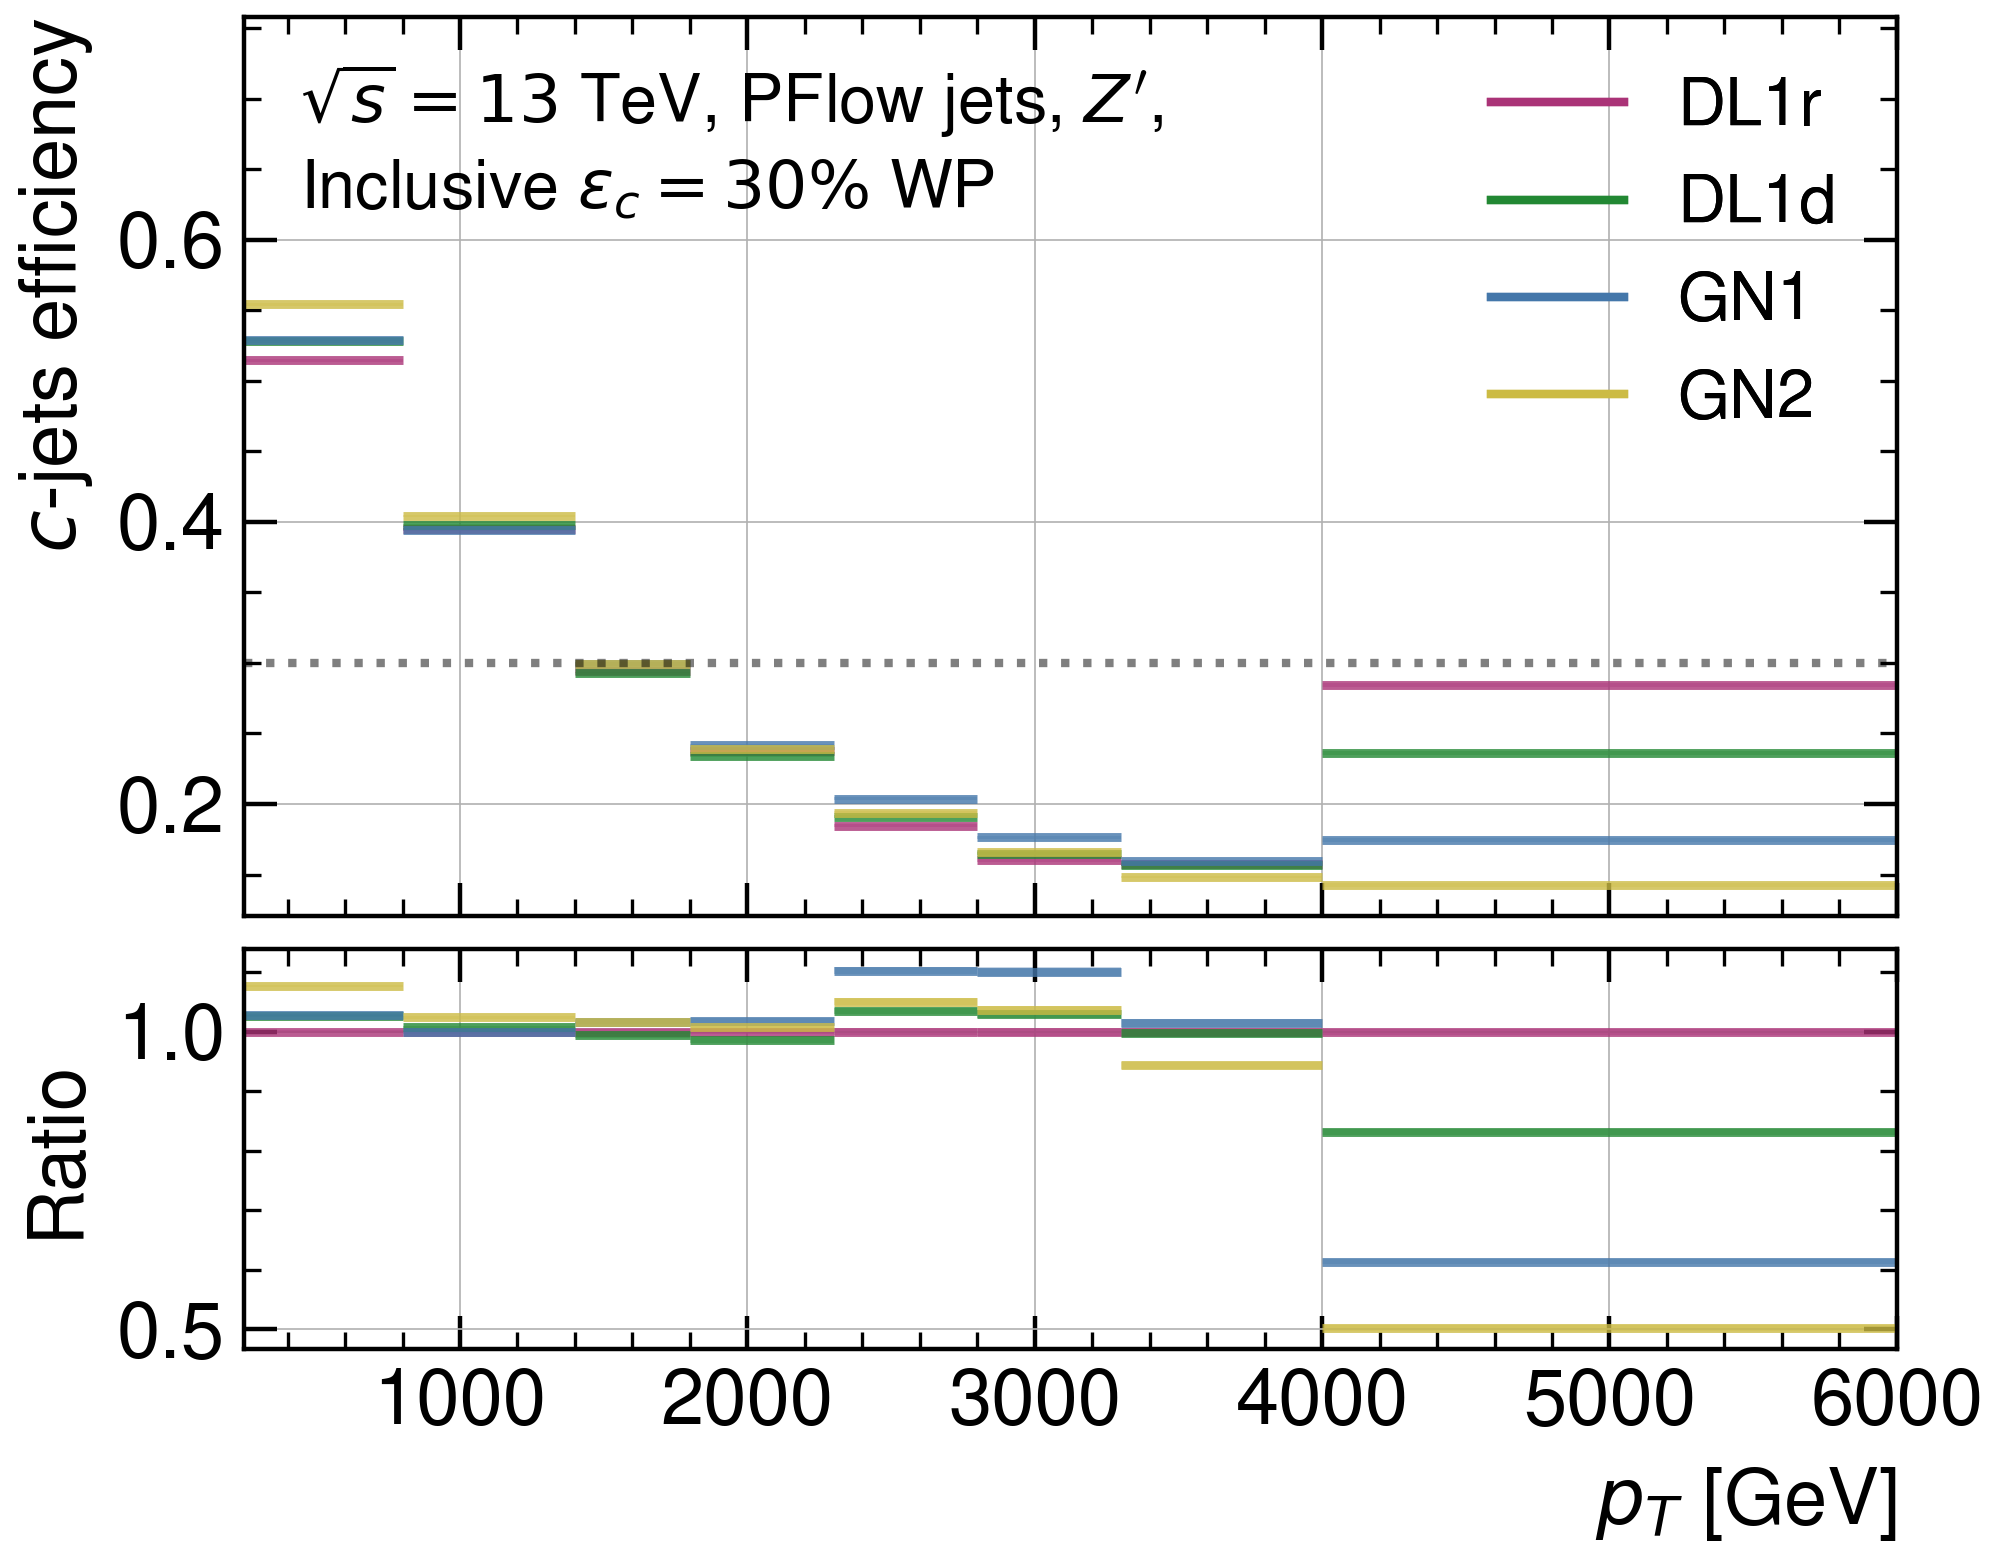
\includegraphics[width=0.48\textwidth]{Images/FTAG/GN/GN2/pt_plots/pt_zp_c_eff.png}
    \caption{Comparing the different models $c$-tagging efficiency as a function of jet $p_T$ for the inclusive $c$-tagging 30\% working point on the $t\bar{t}$ (left) and $Z'$ (right). The flavour fraction is set at $f^c_b = 0.2$ for all taggers.}
    \label{apfig:GNxptc_eff}
\end{figure} 

Figure \ref{apfig:GNxptc_efffixedl} presents the $c$-tagging efficiency per bin for a per bin light-rejection of 50 for $t\bar{t}$ and 10 for $Z'$. The \gls{gn2} performance dominates across the board, except for the highest energy bin of the $Z'$. 

\begin{figure}[h!]
    \centering
    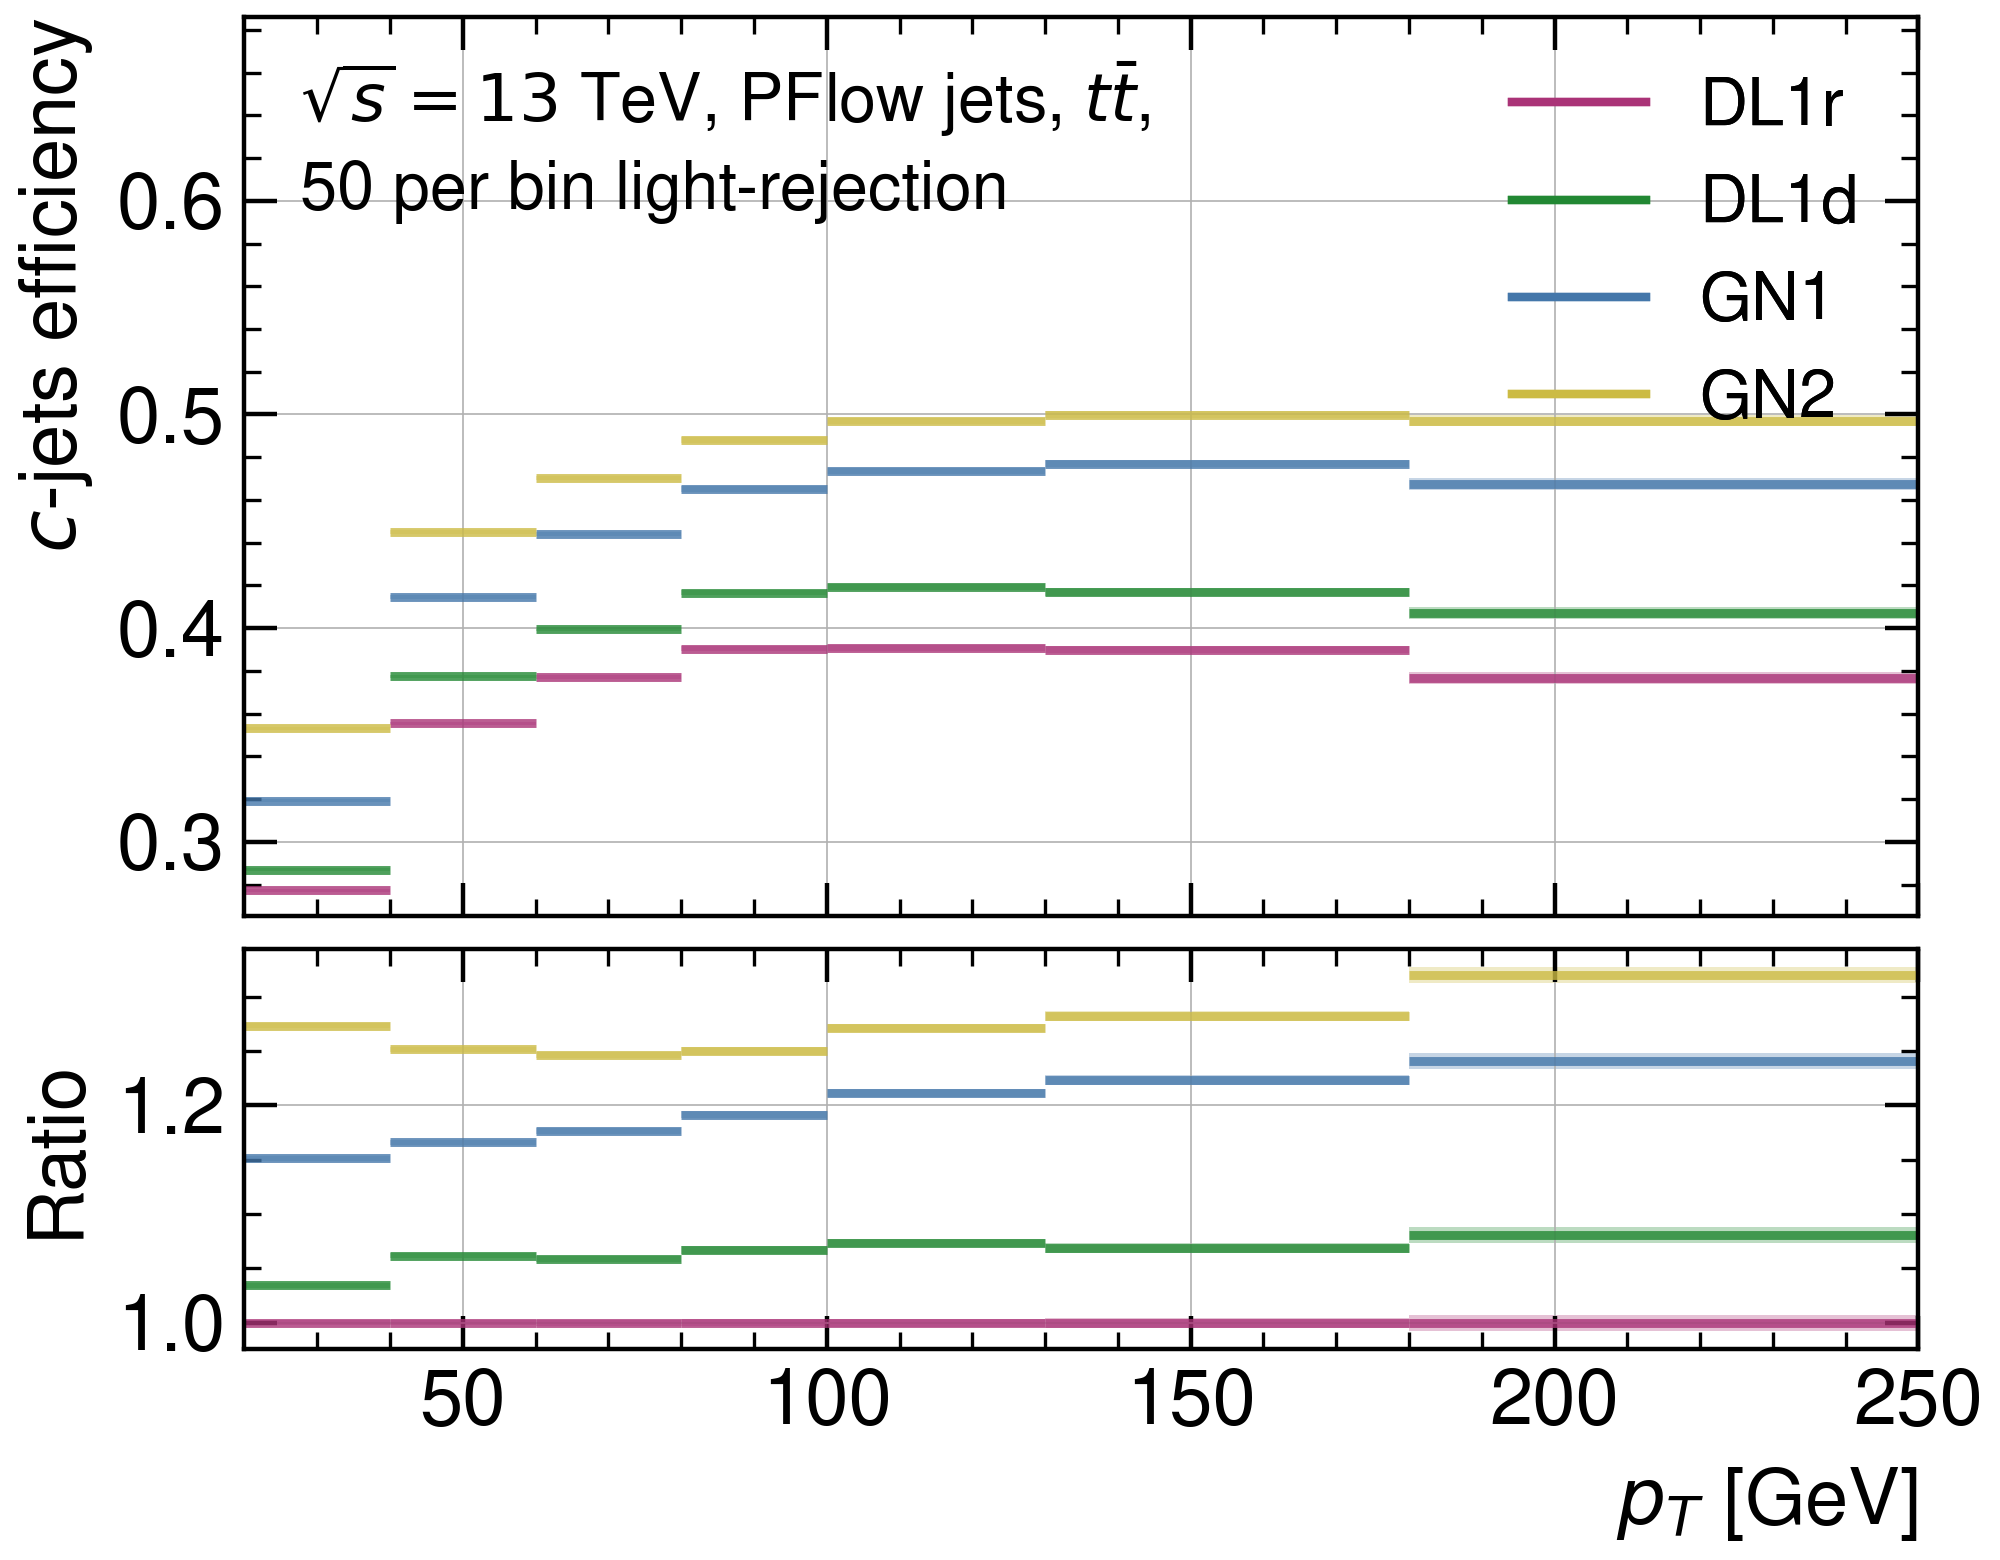
\includegraphics[width=0.48\textwidth]{Images/FTAG/GN/GN2/pt_plots/pt_ttbar_c_eff_fixedlight.png}
    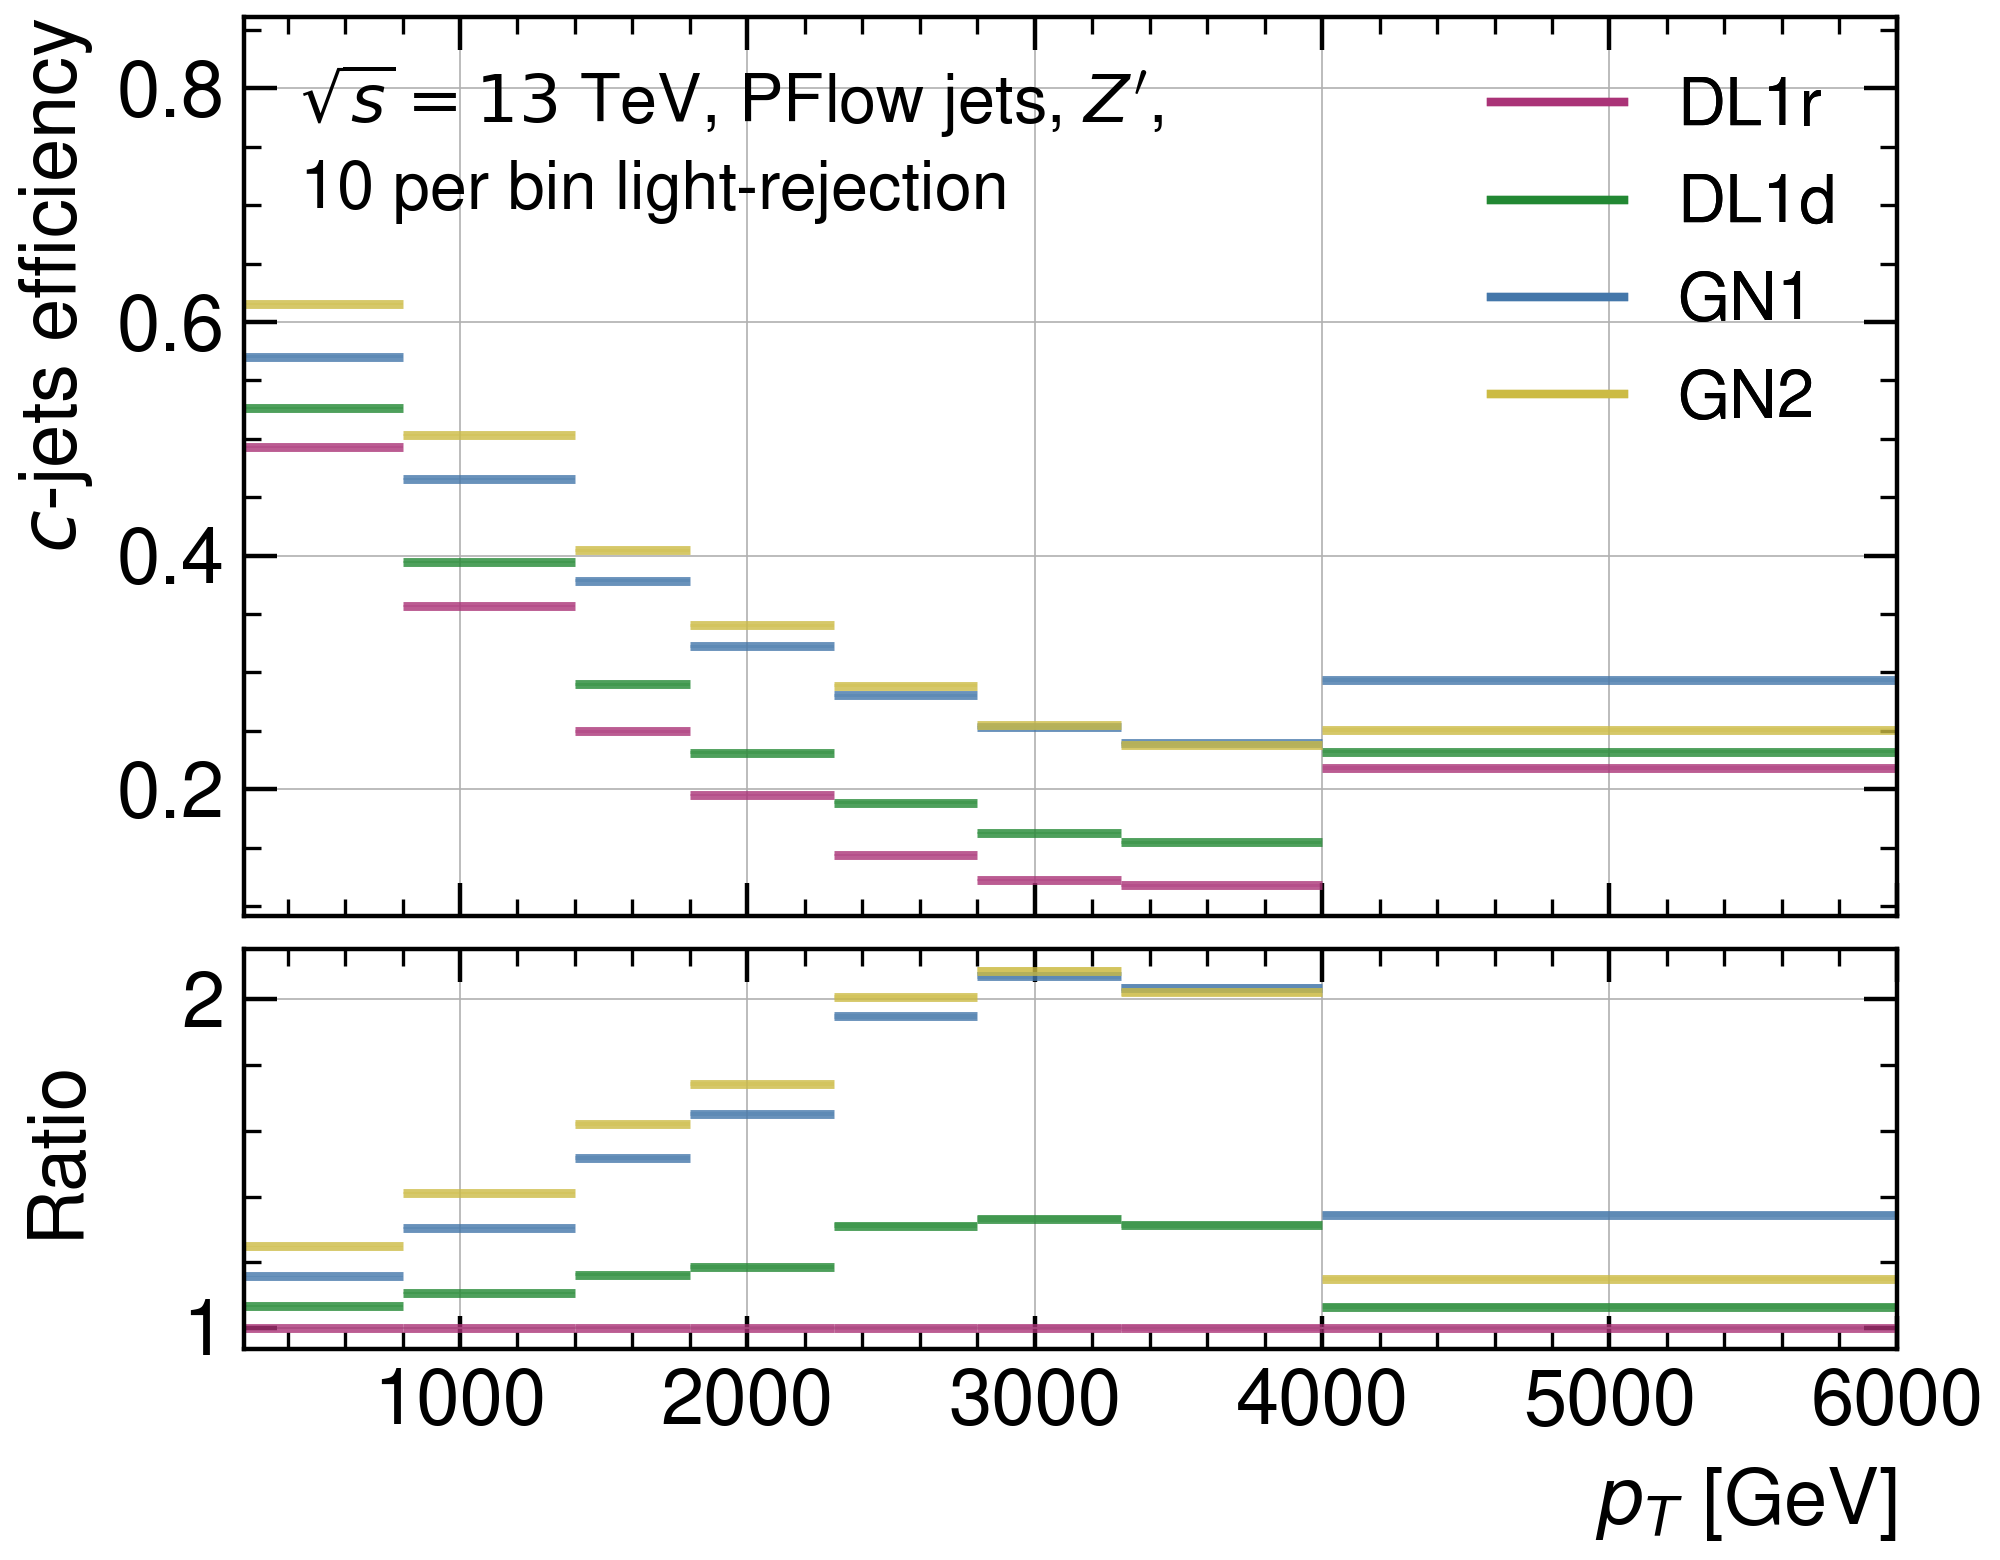
\includegraphics[width=0.48\textwidth]{Images/FTAG/GN/GN2/pt_plots/pt_zp_c_eff_fixedlight.png}
    \caption{Comparing the different models $c$-tagging efficiency as a function of jet $p_T$ at a fixed light-jet rejection per bin of 50 for the $t\bar{t}$ (left) and 10 for the $Z'$ (right) test samples. The flavour fraction is set at $f^c_b = 0.2$ for all taggers.}
    \label{apfig:GNxptc_efffixedl}
  \end{figure} 

Figures \ref{apfig:GNxptc_efffixedl} presents the $c$- and light-rejection at an inclusive 70\% $b$-tagging \gls{wp}. The equivalent information for $c$-tagging at a $c$-tagging \gls{wp} of 30\% is displayed in Figures \ref{apfig:GNxptc_brej} and \ref{apfig:GNxptc_urej} for $b$- and light-rejection. 
% Rej c - btagging
\begin{figure}[h!]
    \centering
    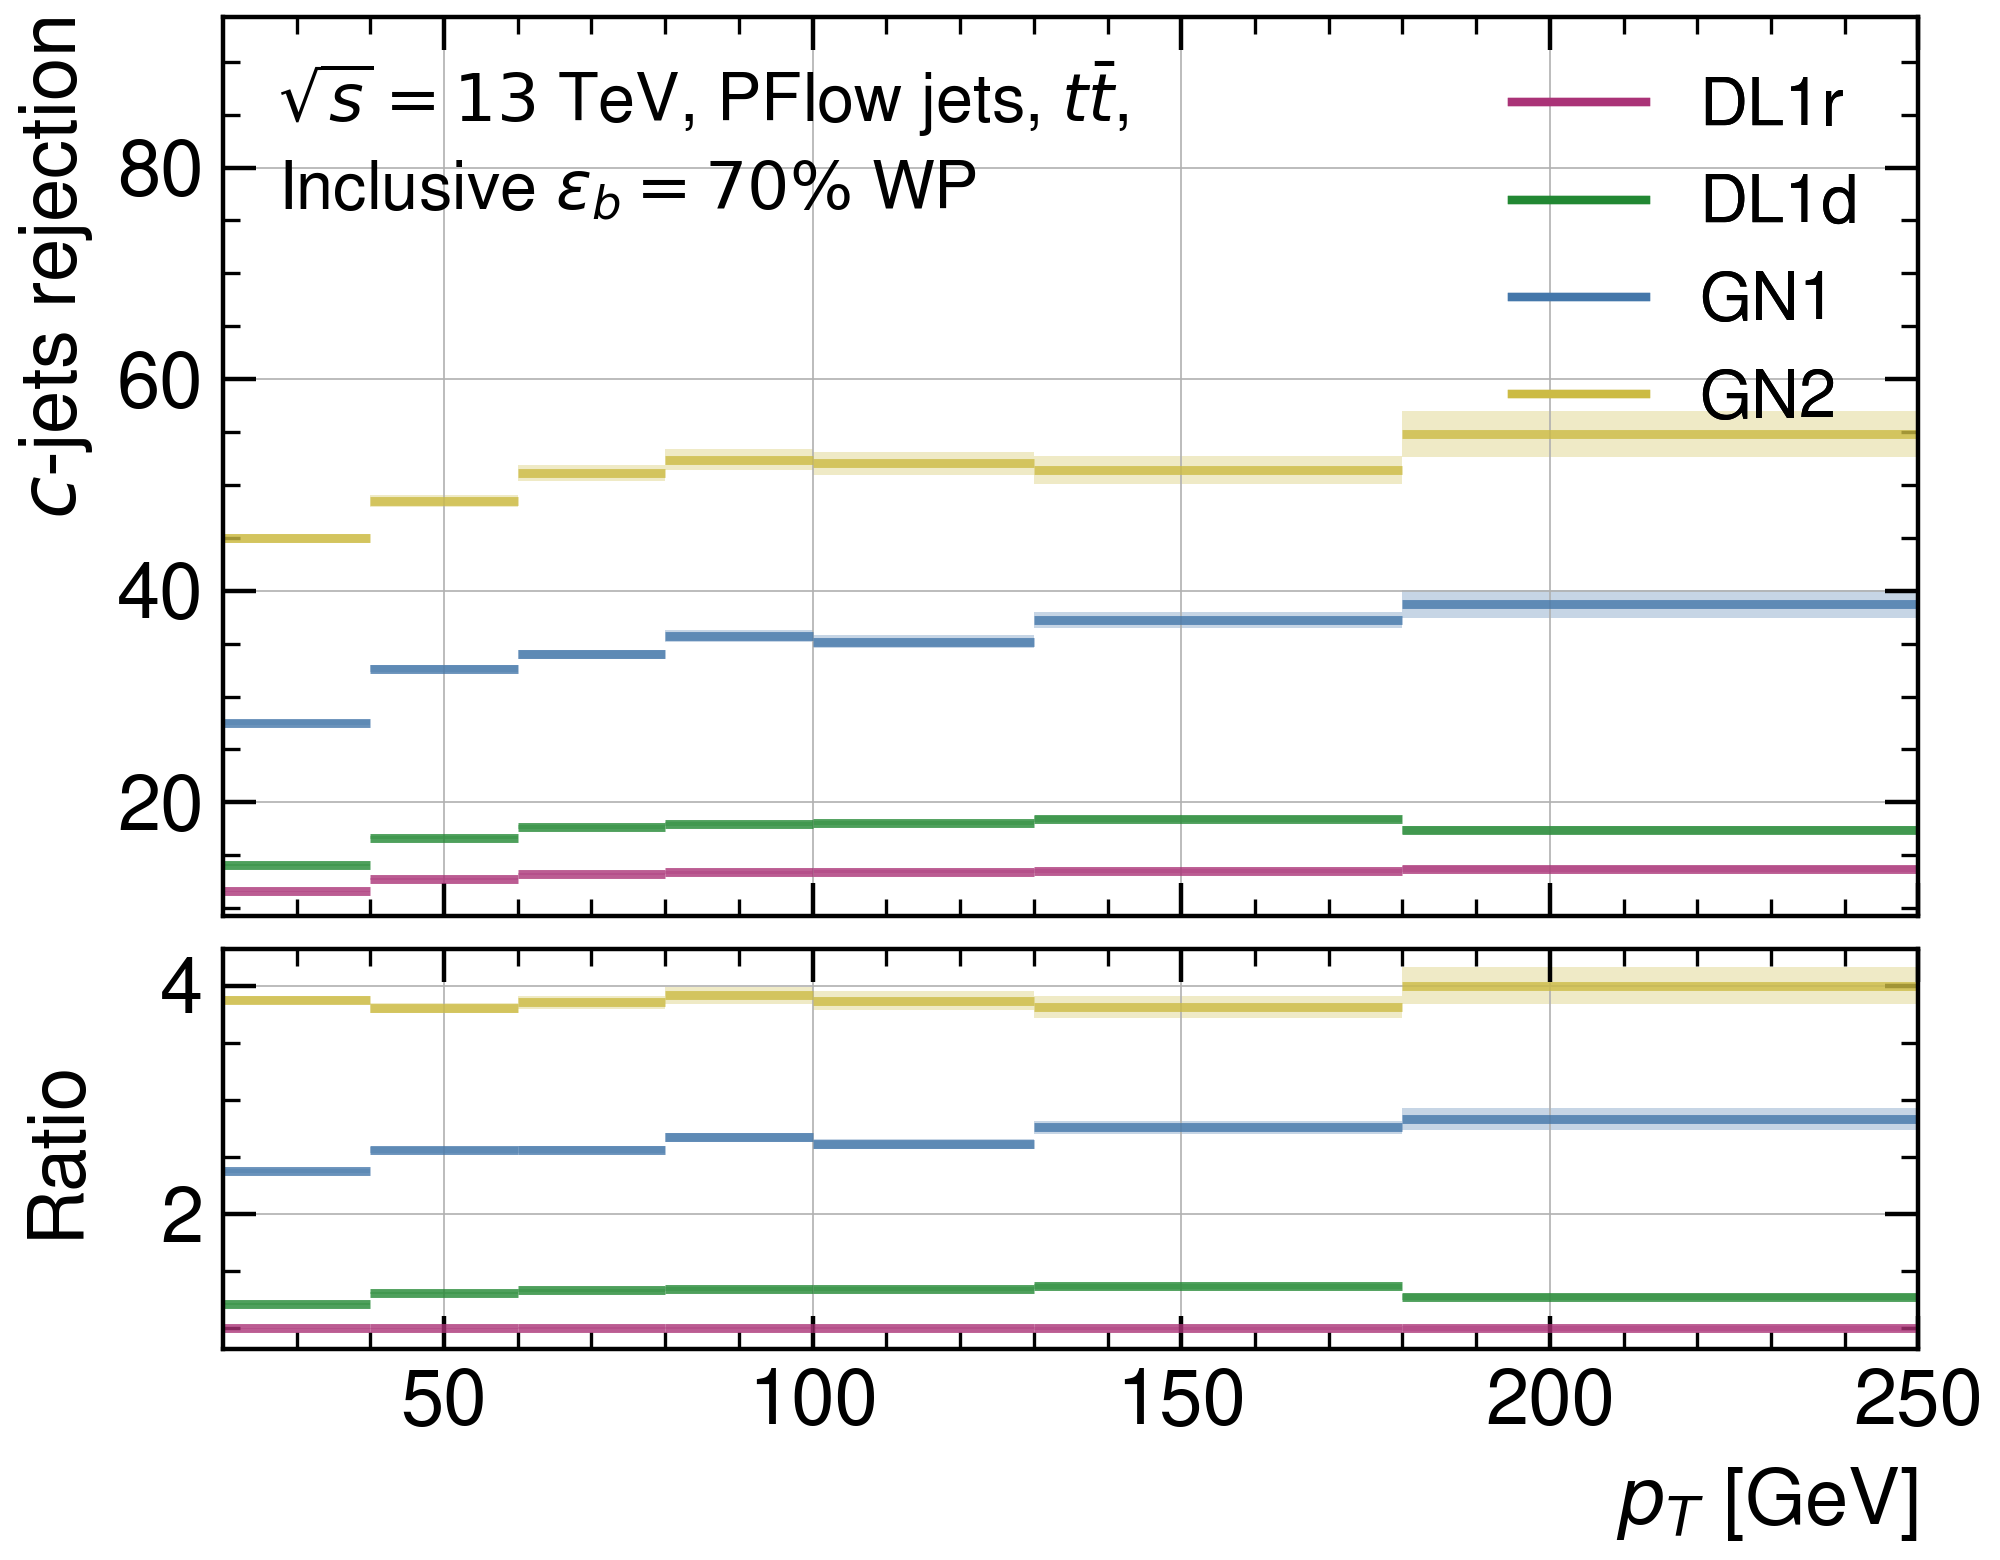
\includegraphics[width=0.48\textwidth]{Images/FTAG/GN/GN2/pt_plots/pt_ttbar_c_rej.png}
    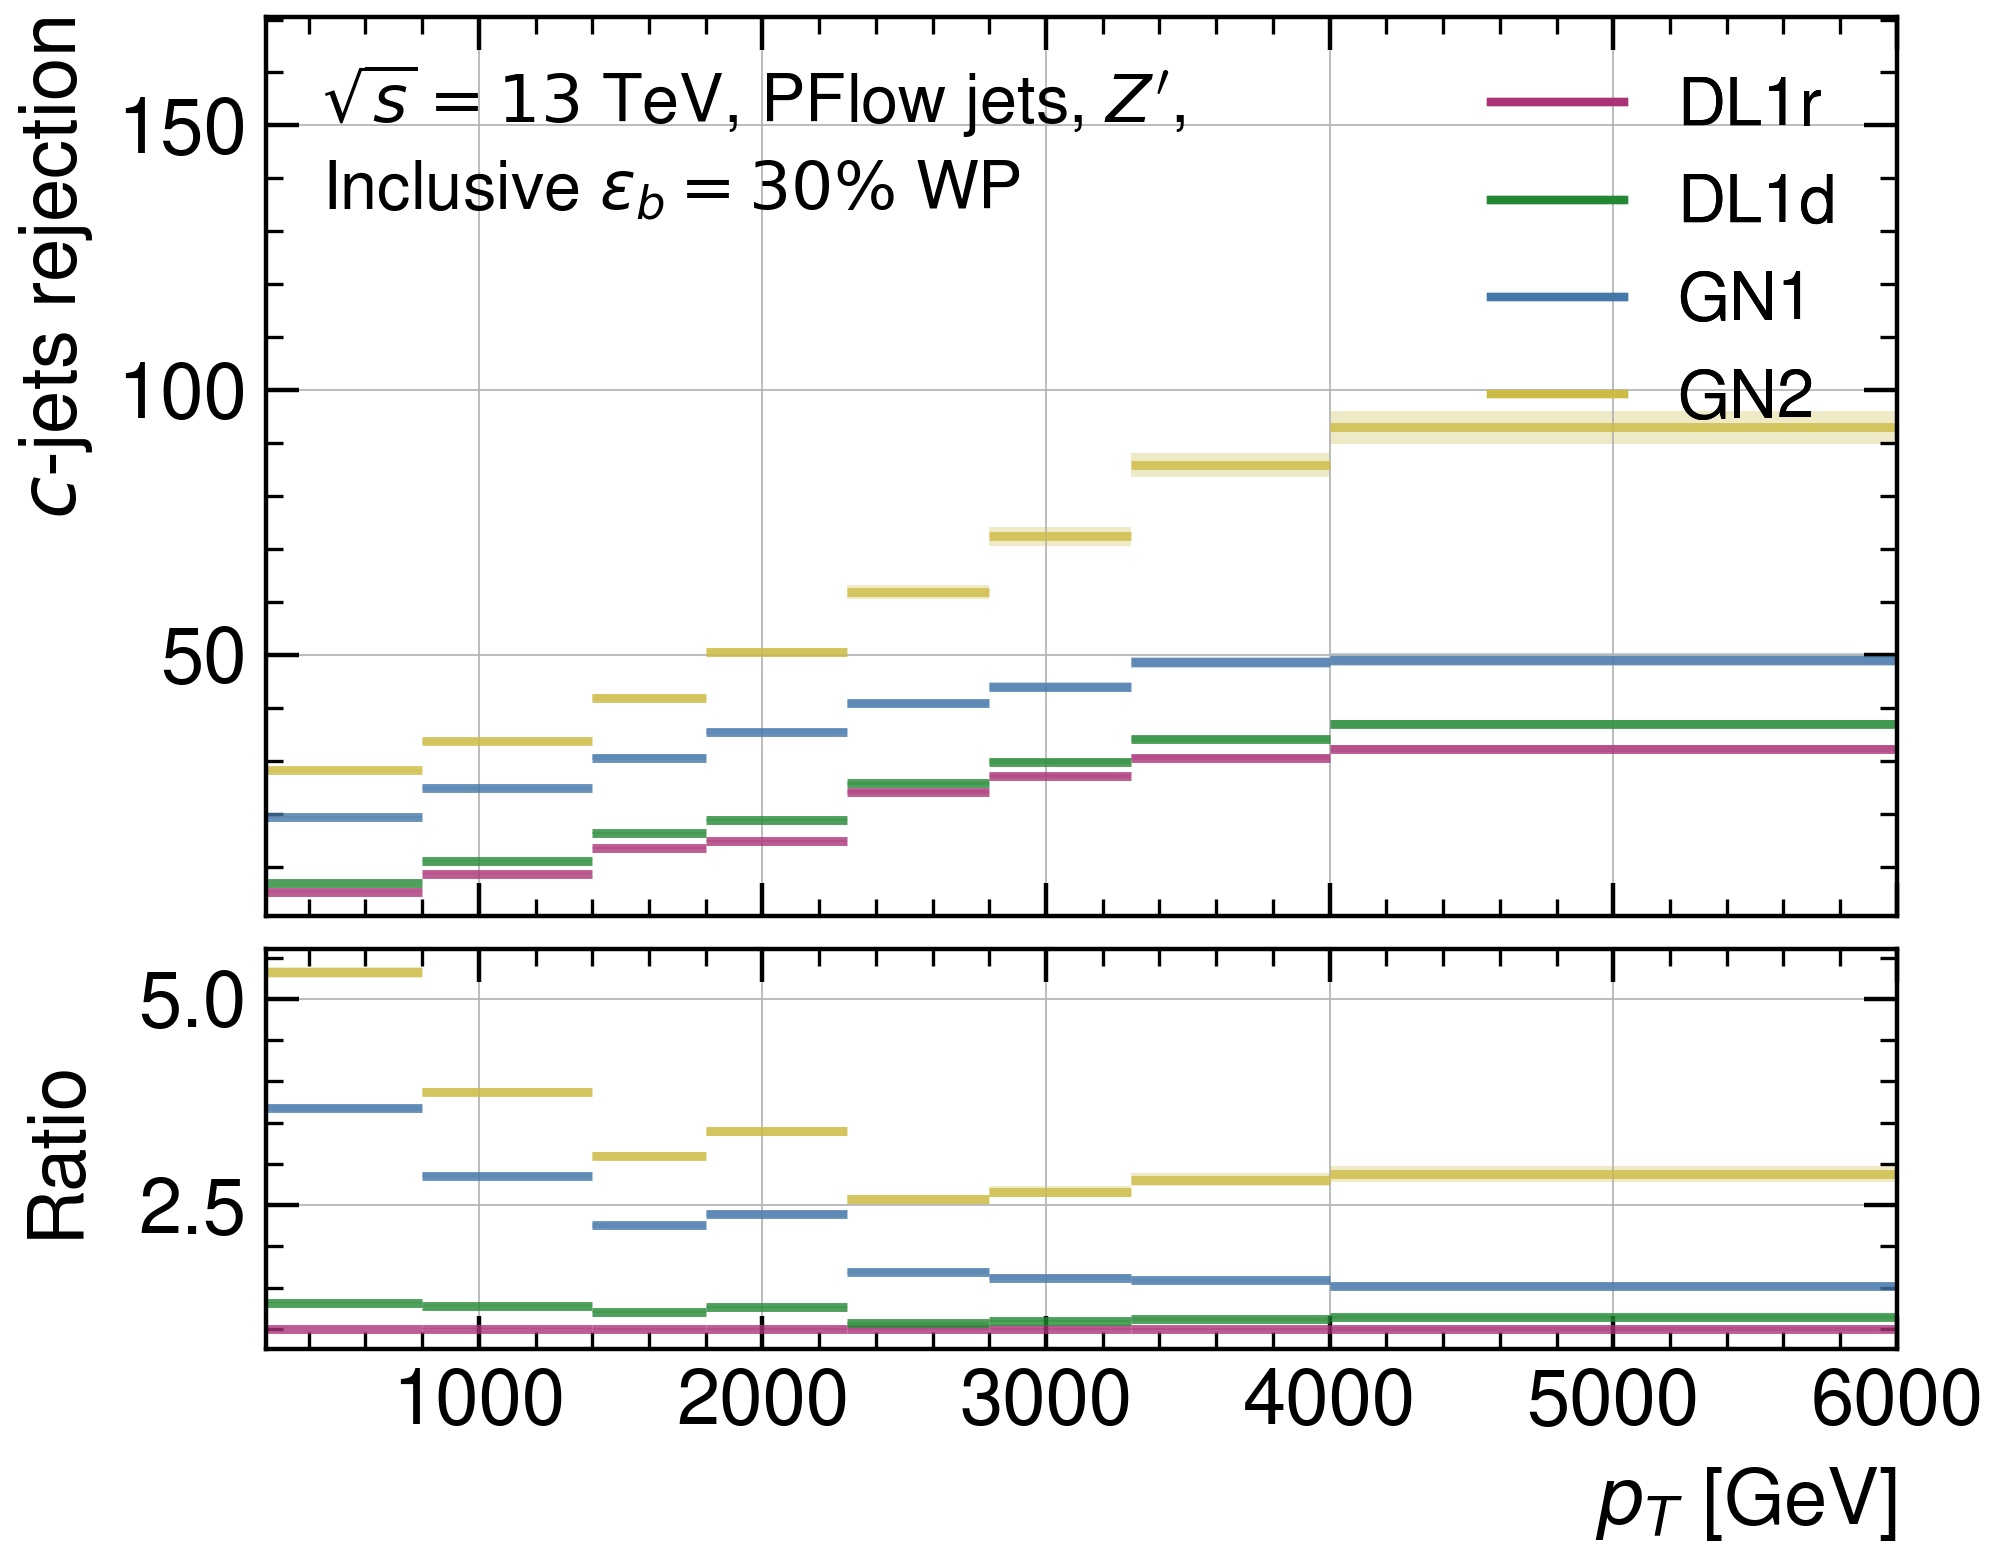
\includegraphics[width=0.48\textwidth]{Images/FTAG/GN/GN2/pt_plots/pt_zp_c_rej.png}
    \caption{Comparing the different models $c$-rejection as a function of jet $p_T$ for the $b$-tagging inclusive 70\% working point on the $t\bar{t}$ (left) and 30\% working point on $Z'$ (right). The flavour fraction is set at $f^b_c = 0.018$ for DL1r and DL1d, 0.05 for GN1, and 0.1 for GN2.}
    \label{apfig:GNxptb_crej}
  \end{figure} 
  
  % Rej light - btagging
  \begin{figure}[h!]
    \centering
    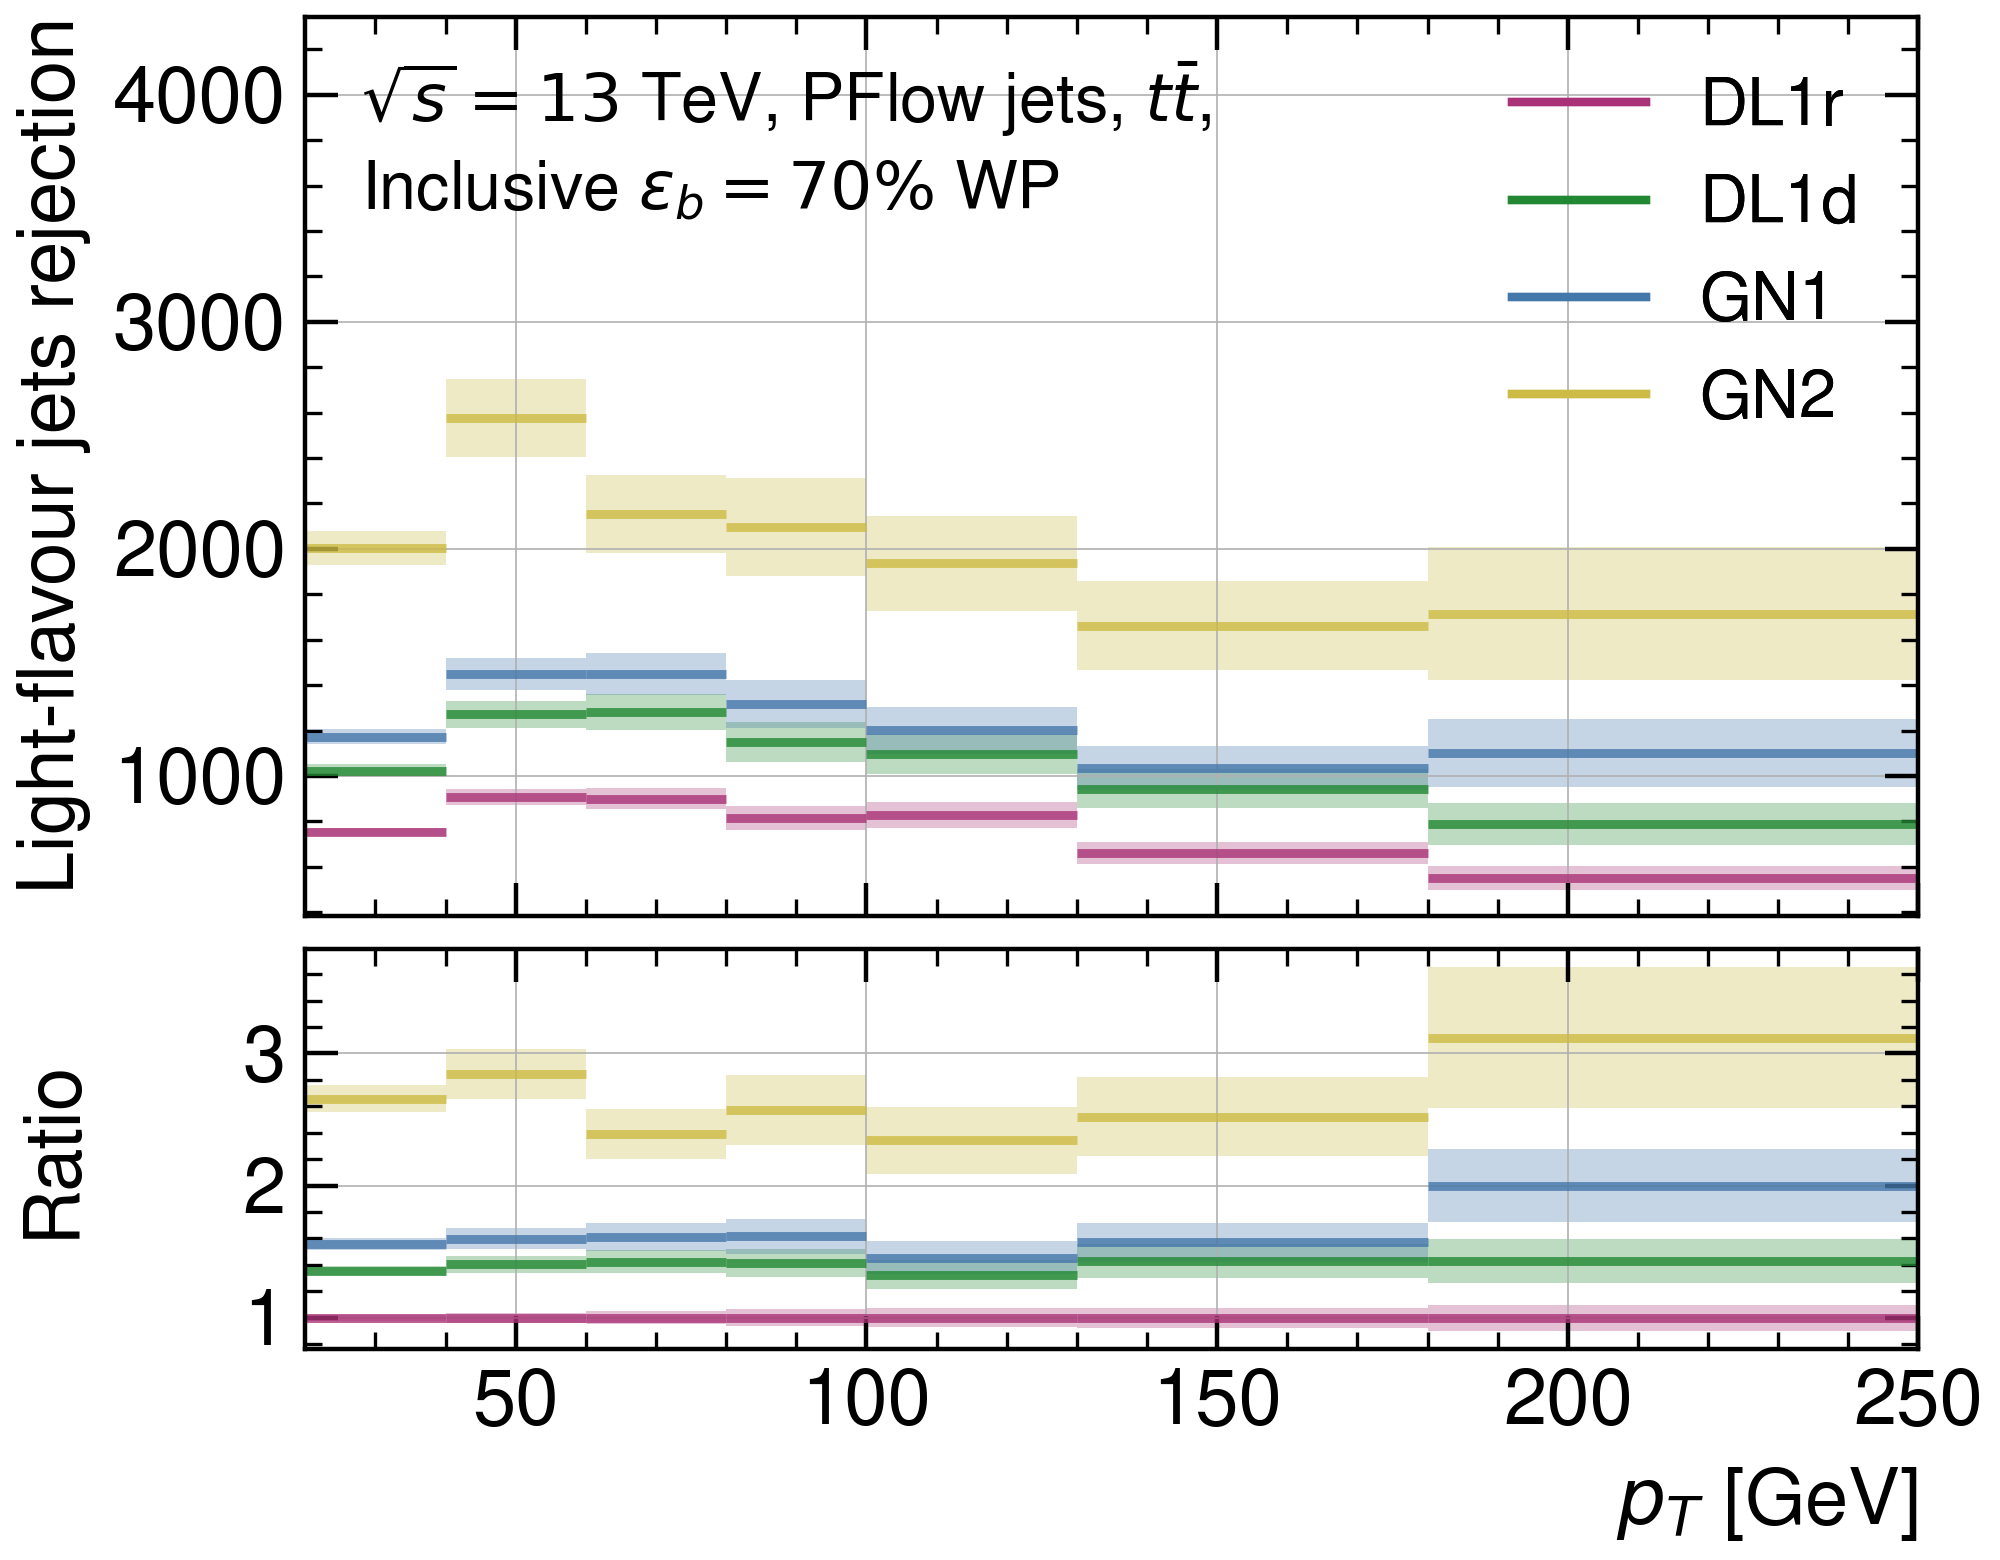
\includegraphics[width=0.48\textwidth]{Images/FTAG/GN/GN2/pt_plots/pt_ttbar_light_rej.png}
    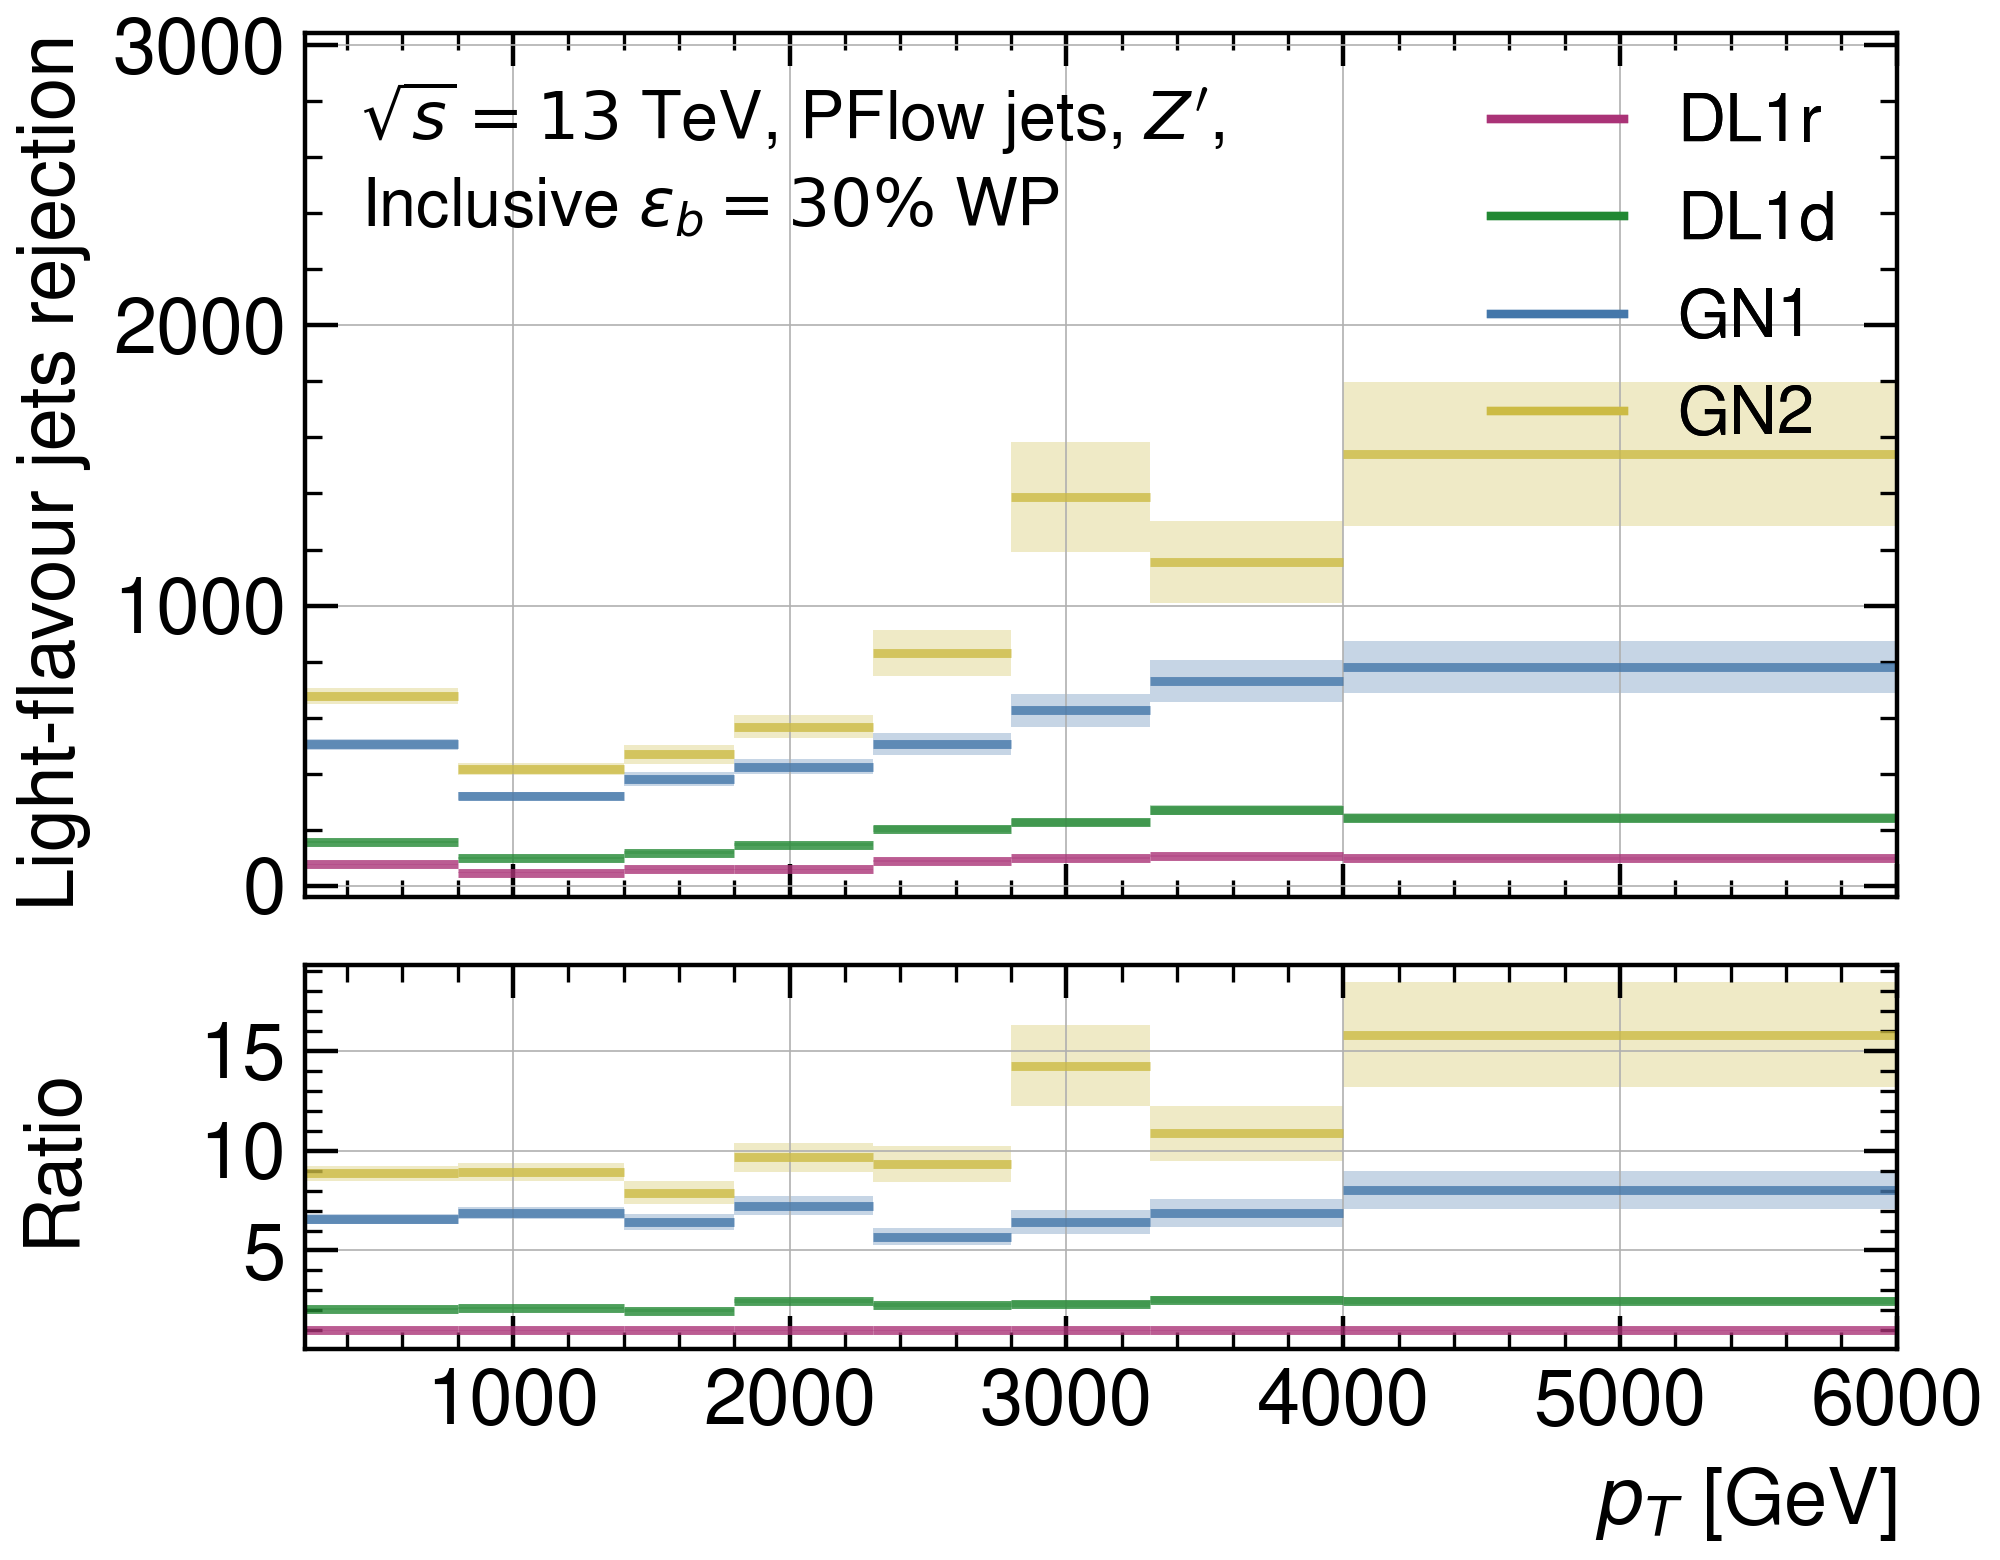
\includegraphics[width=0.48\textwidth]{Images/FTAG/GN/GN2/pt_plots/pt_zp_light_rej.png}
    \caption{Comparing the different models light-rejection as a function of jet $p_T$ for the $b$-tagging inclusive 70\% working point on the $t\bar{t}$ (left) and 30\% working point on $Z'$ (right). The flavour fraction is set at $f^b_c = 0.018$ for DL1r and DL1d, 0.05 for GN1, and 0.1 for GN2.}
    \label{apfig:GNxptb_urej}
  \end{figure} 
  
% Rej b - ctagging
\begin{figure}[h!]
    \centering
    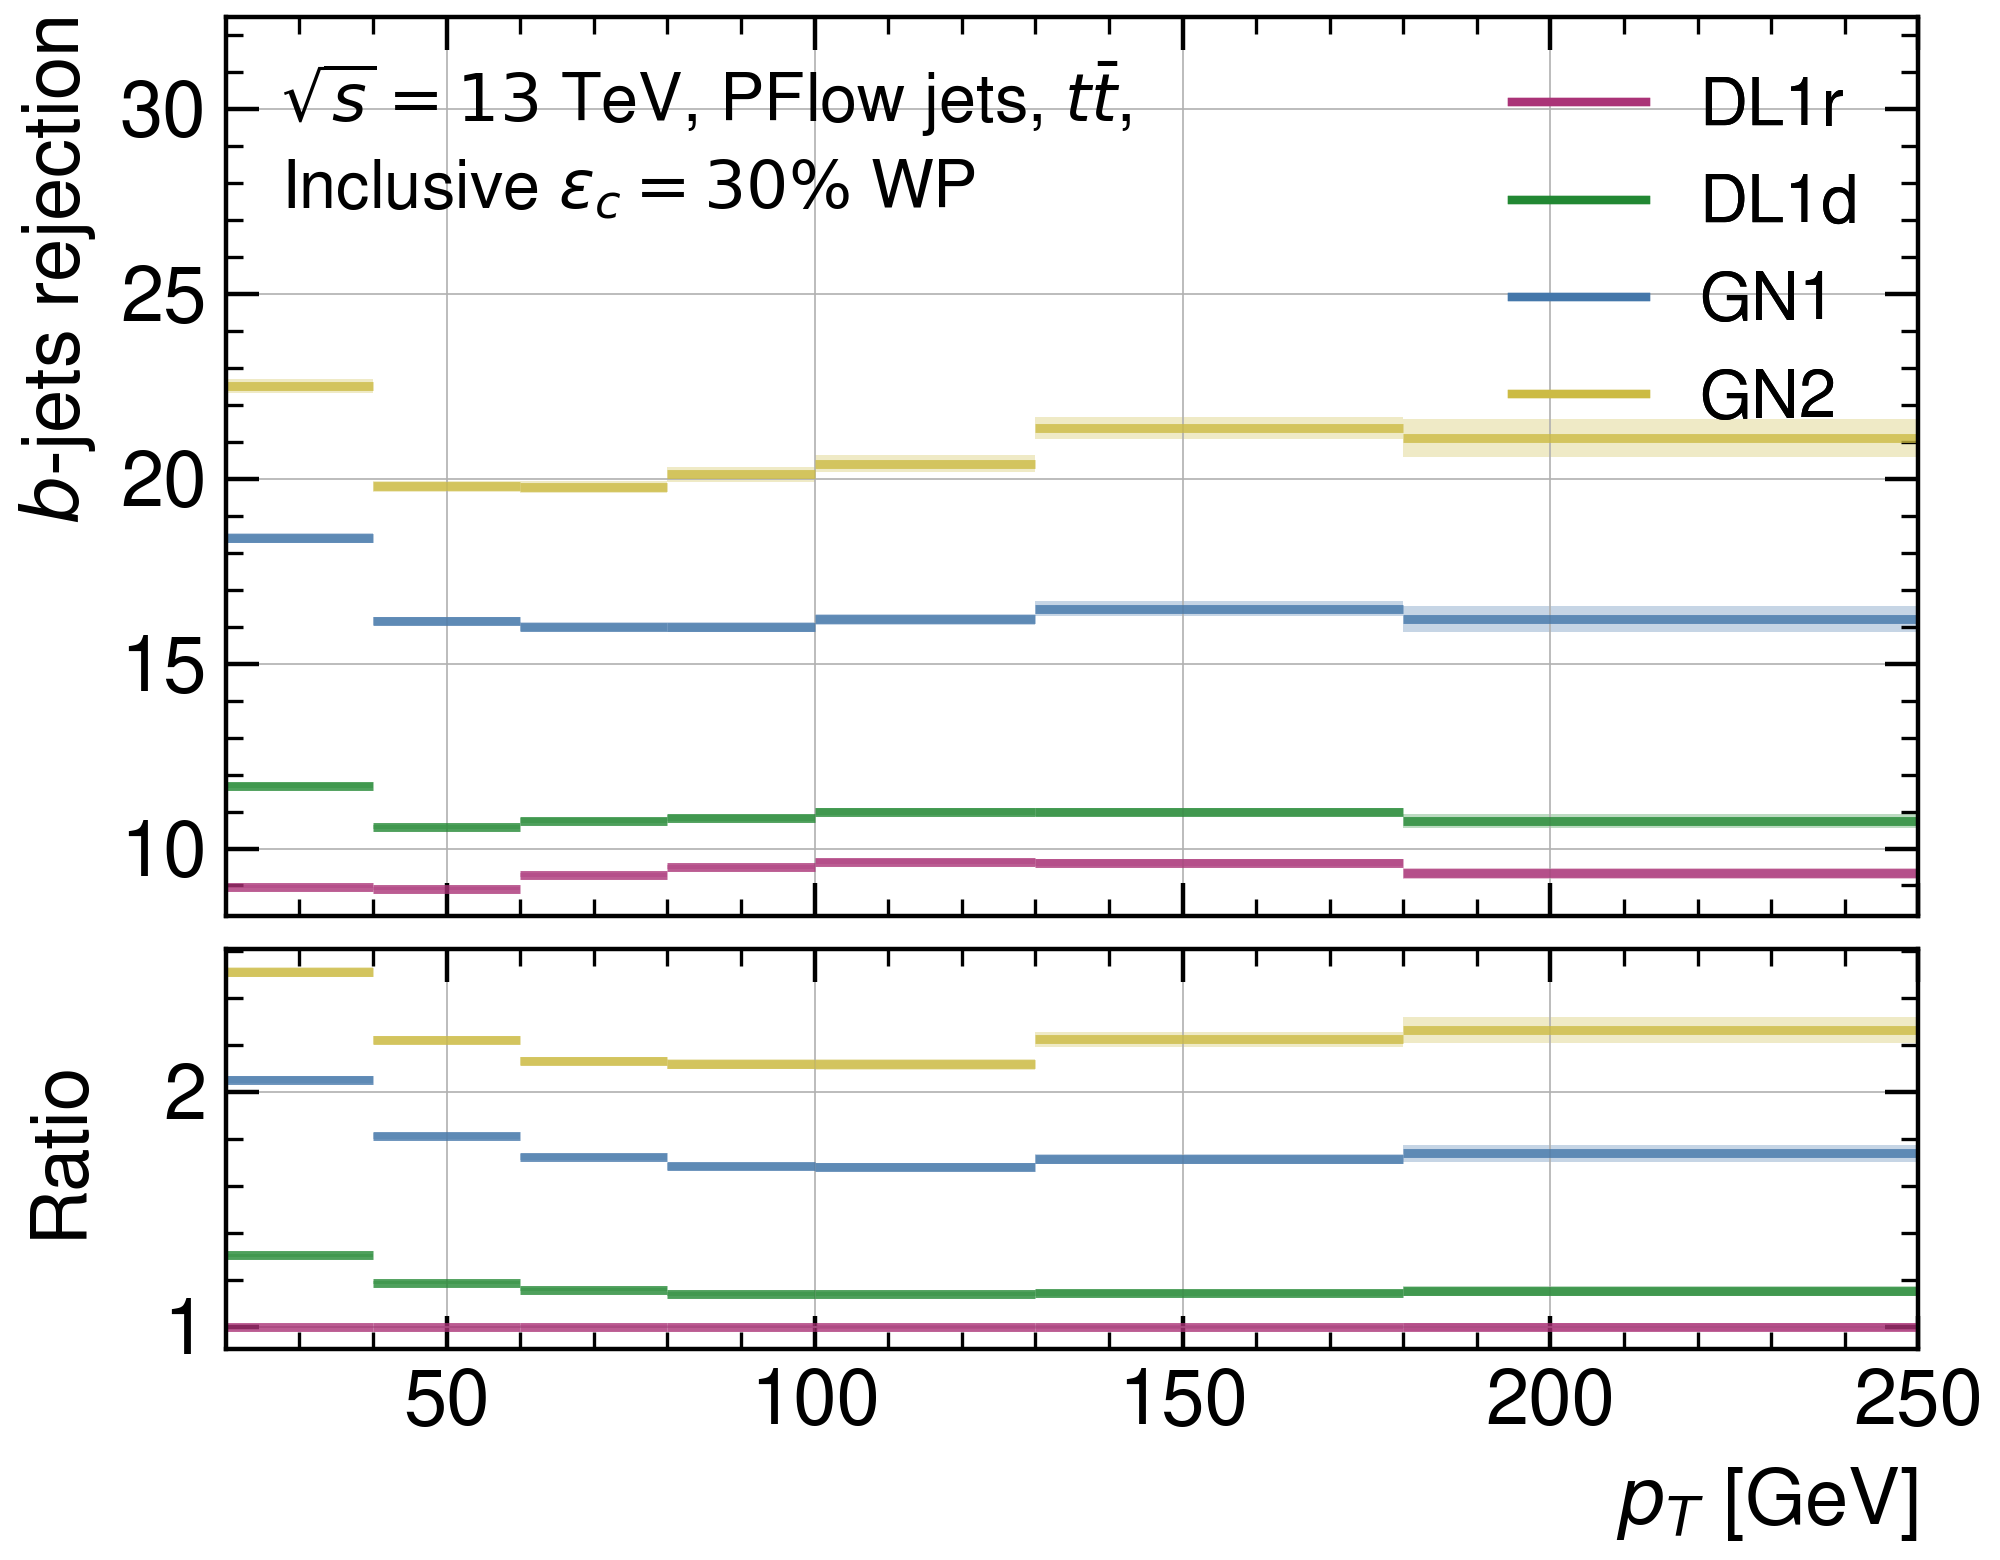
\includegraphics[width=0.48\textwidth]{Images/FTAG/GN/GN2/pt_plots/pt_ttbar_b_rej_c.png}
    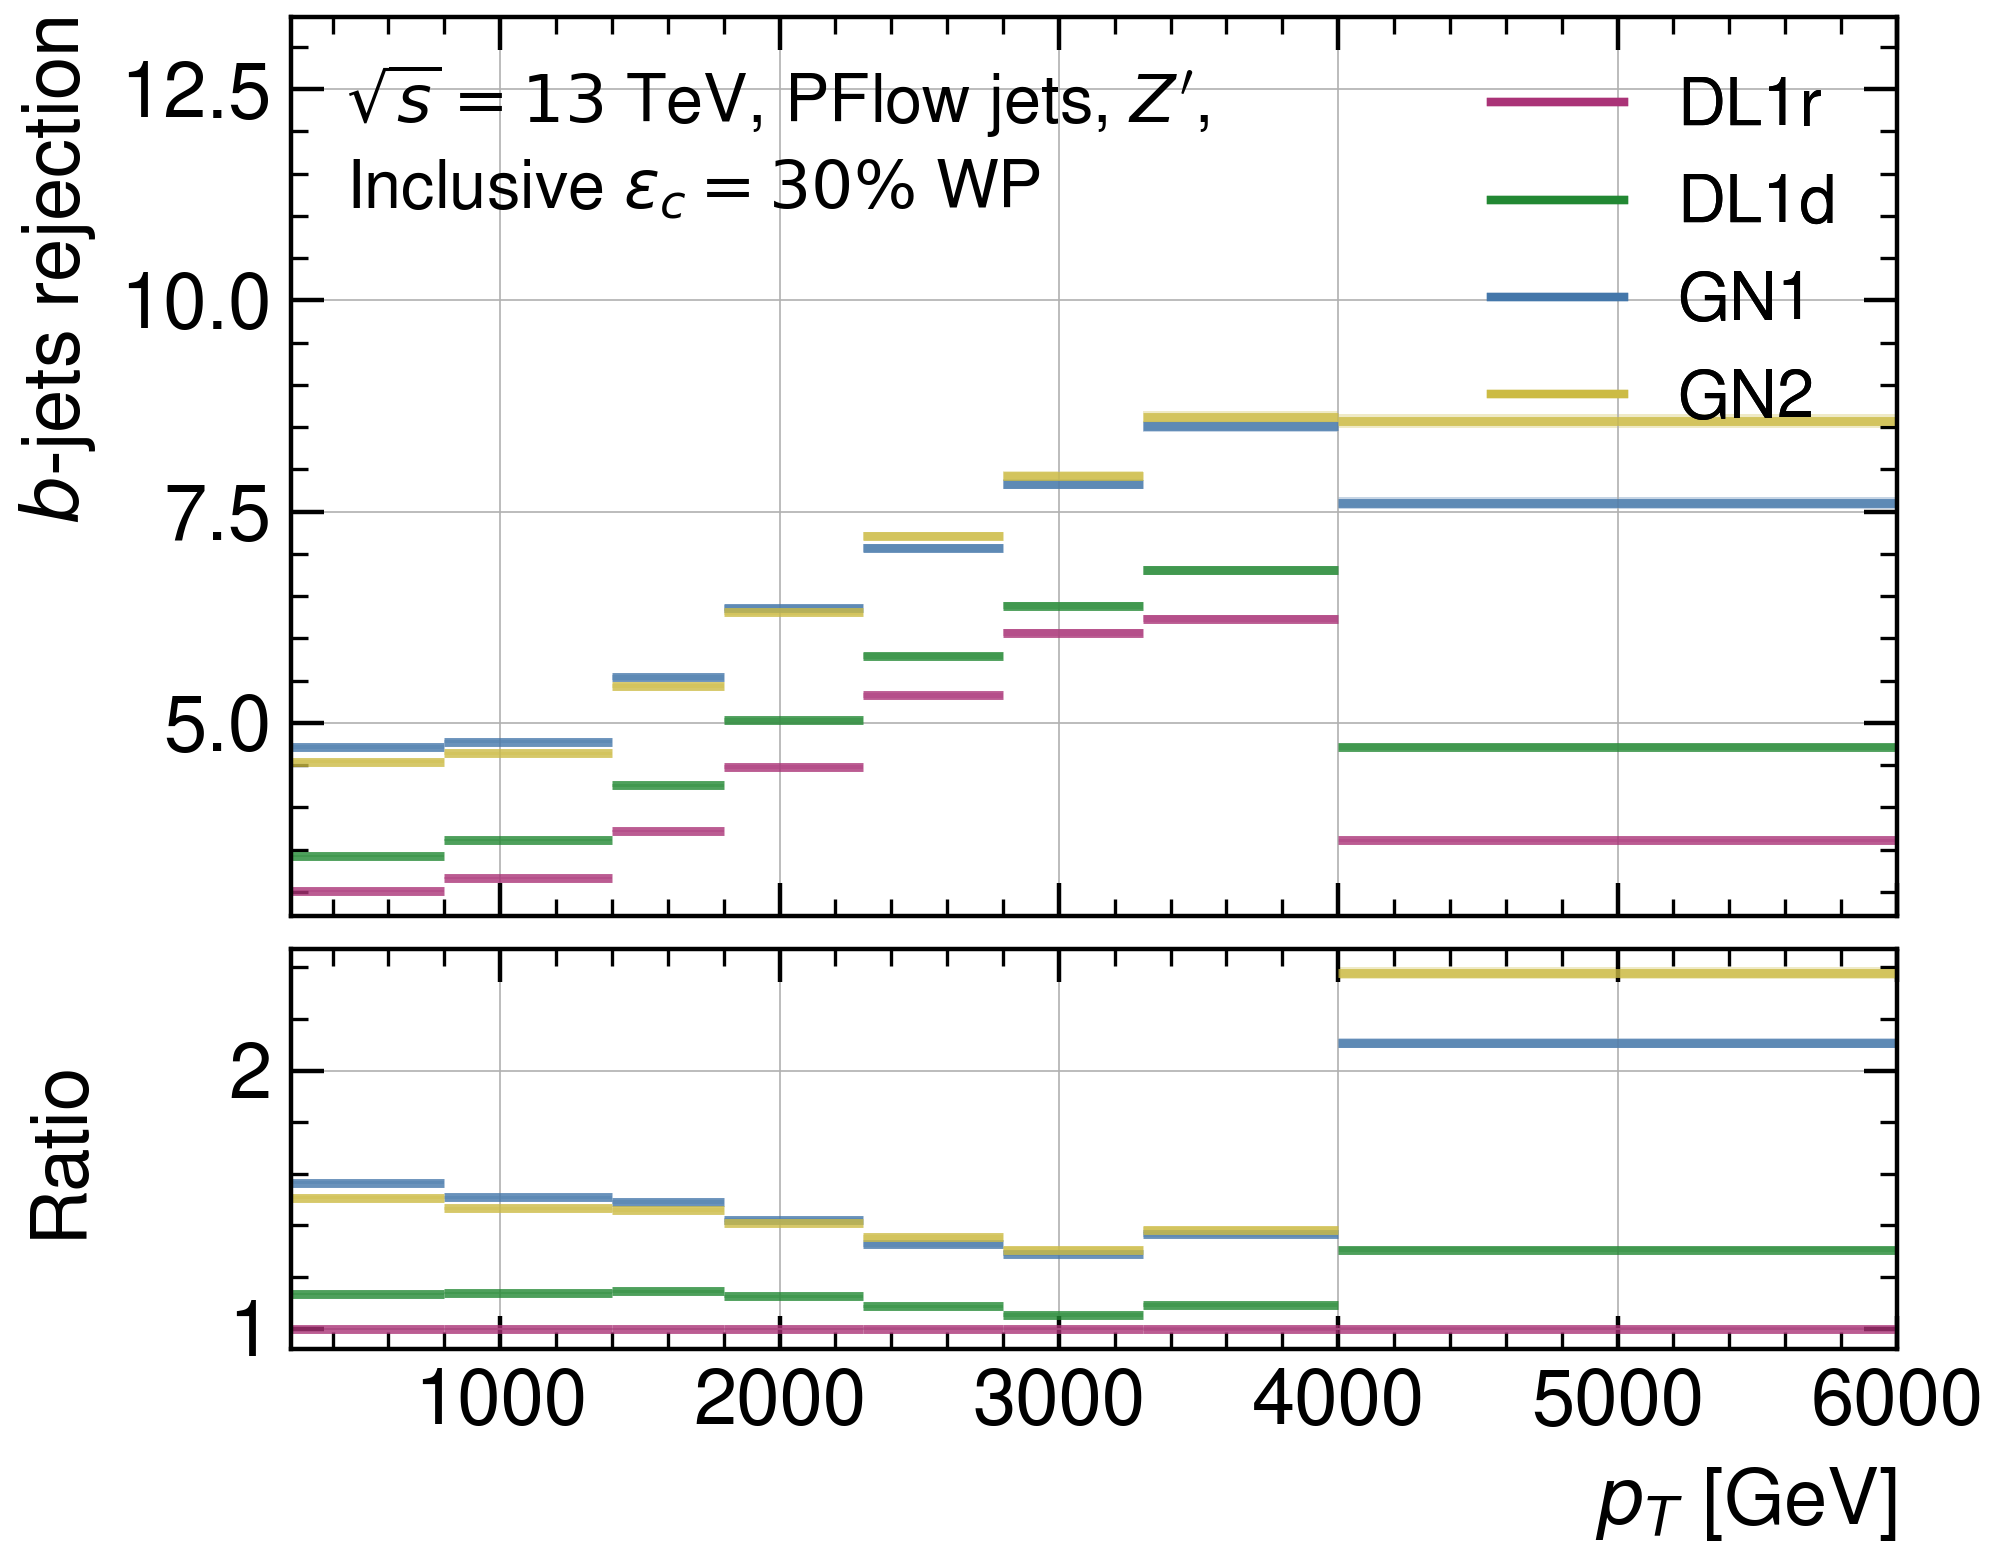
\includegraphics[width=0.48\textwidth]{Images/FTAG/GN/GN2/pt_plots/pt_zp_b_rej_c.png}
    \caption{Comparing the different models $b$-rejection as a function of jet $p_T$ for the $c$-tagging inclusive 30\% working point on the $t\bar{t}$ (left) and $Z'$ (right). The flavour fraction is set at $f^c_b = 0.2$ for all taggers.}
    \label{apfig:GNxptc_brej}
  \end{figure} 
  
  % Rej light - ctagging
  \begin{figure}[h!]
    \centering
    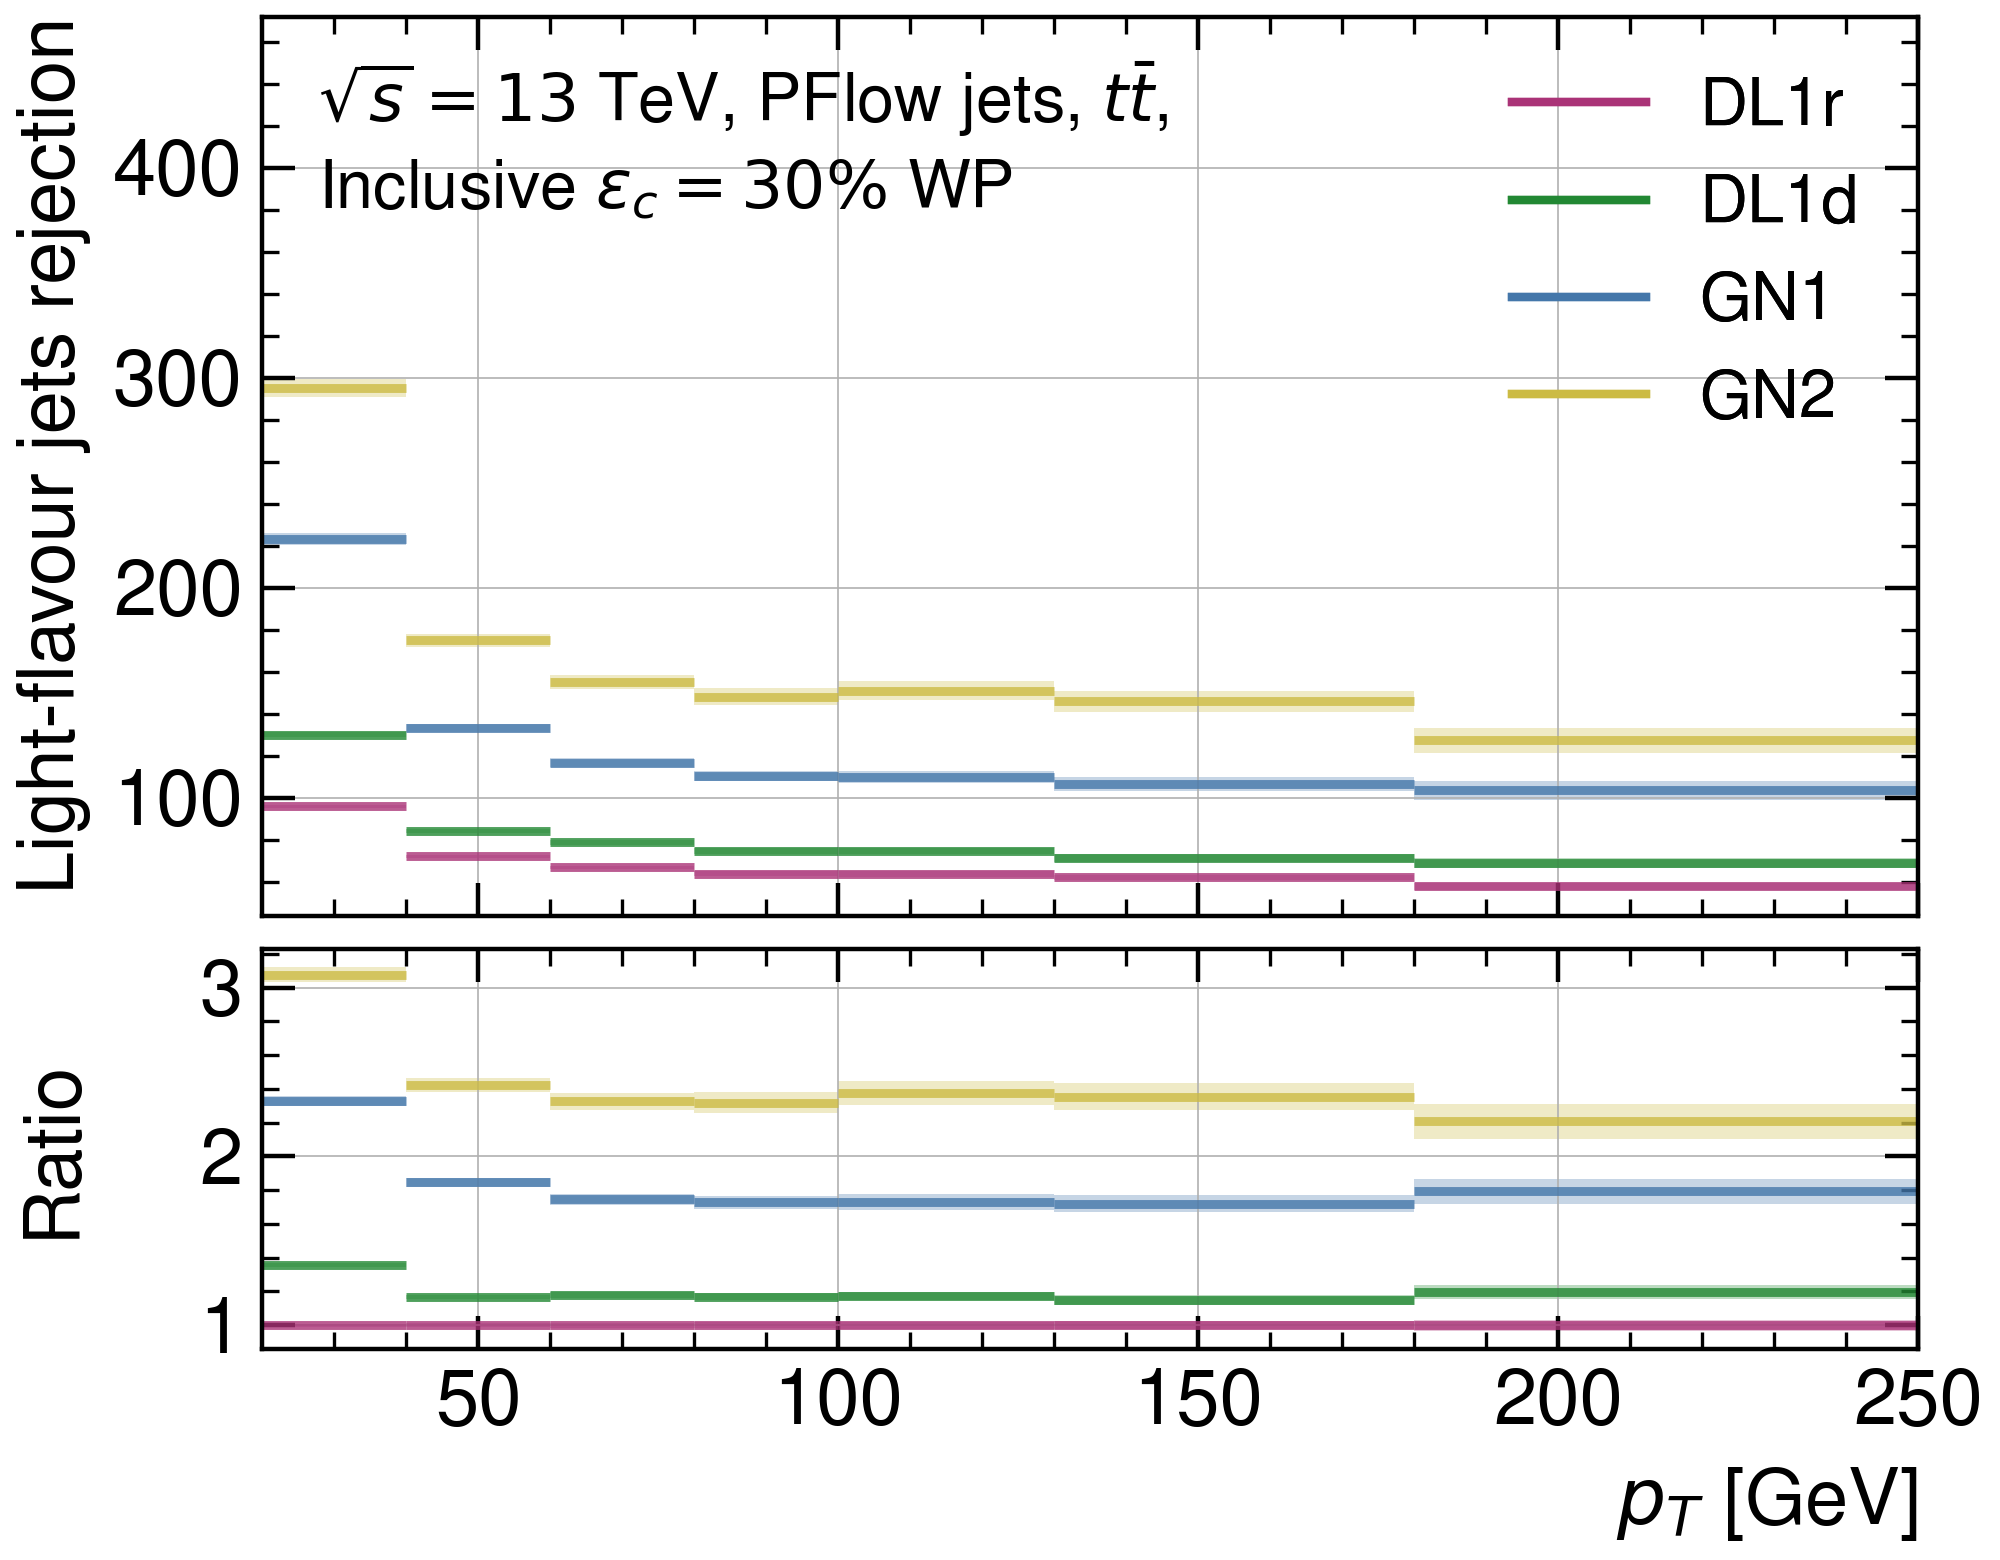
\includegraphics[width=0.48\textwidth]{Images/FTAG/GN/GN2/pt_plots/pt_ttbar_light_rej_c.png}
    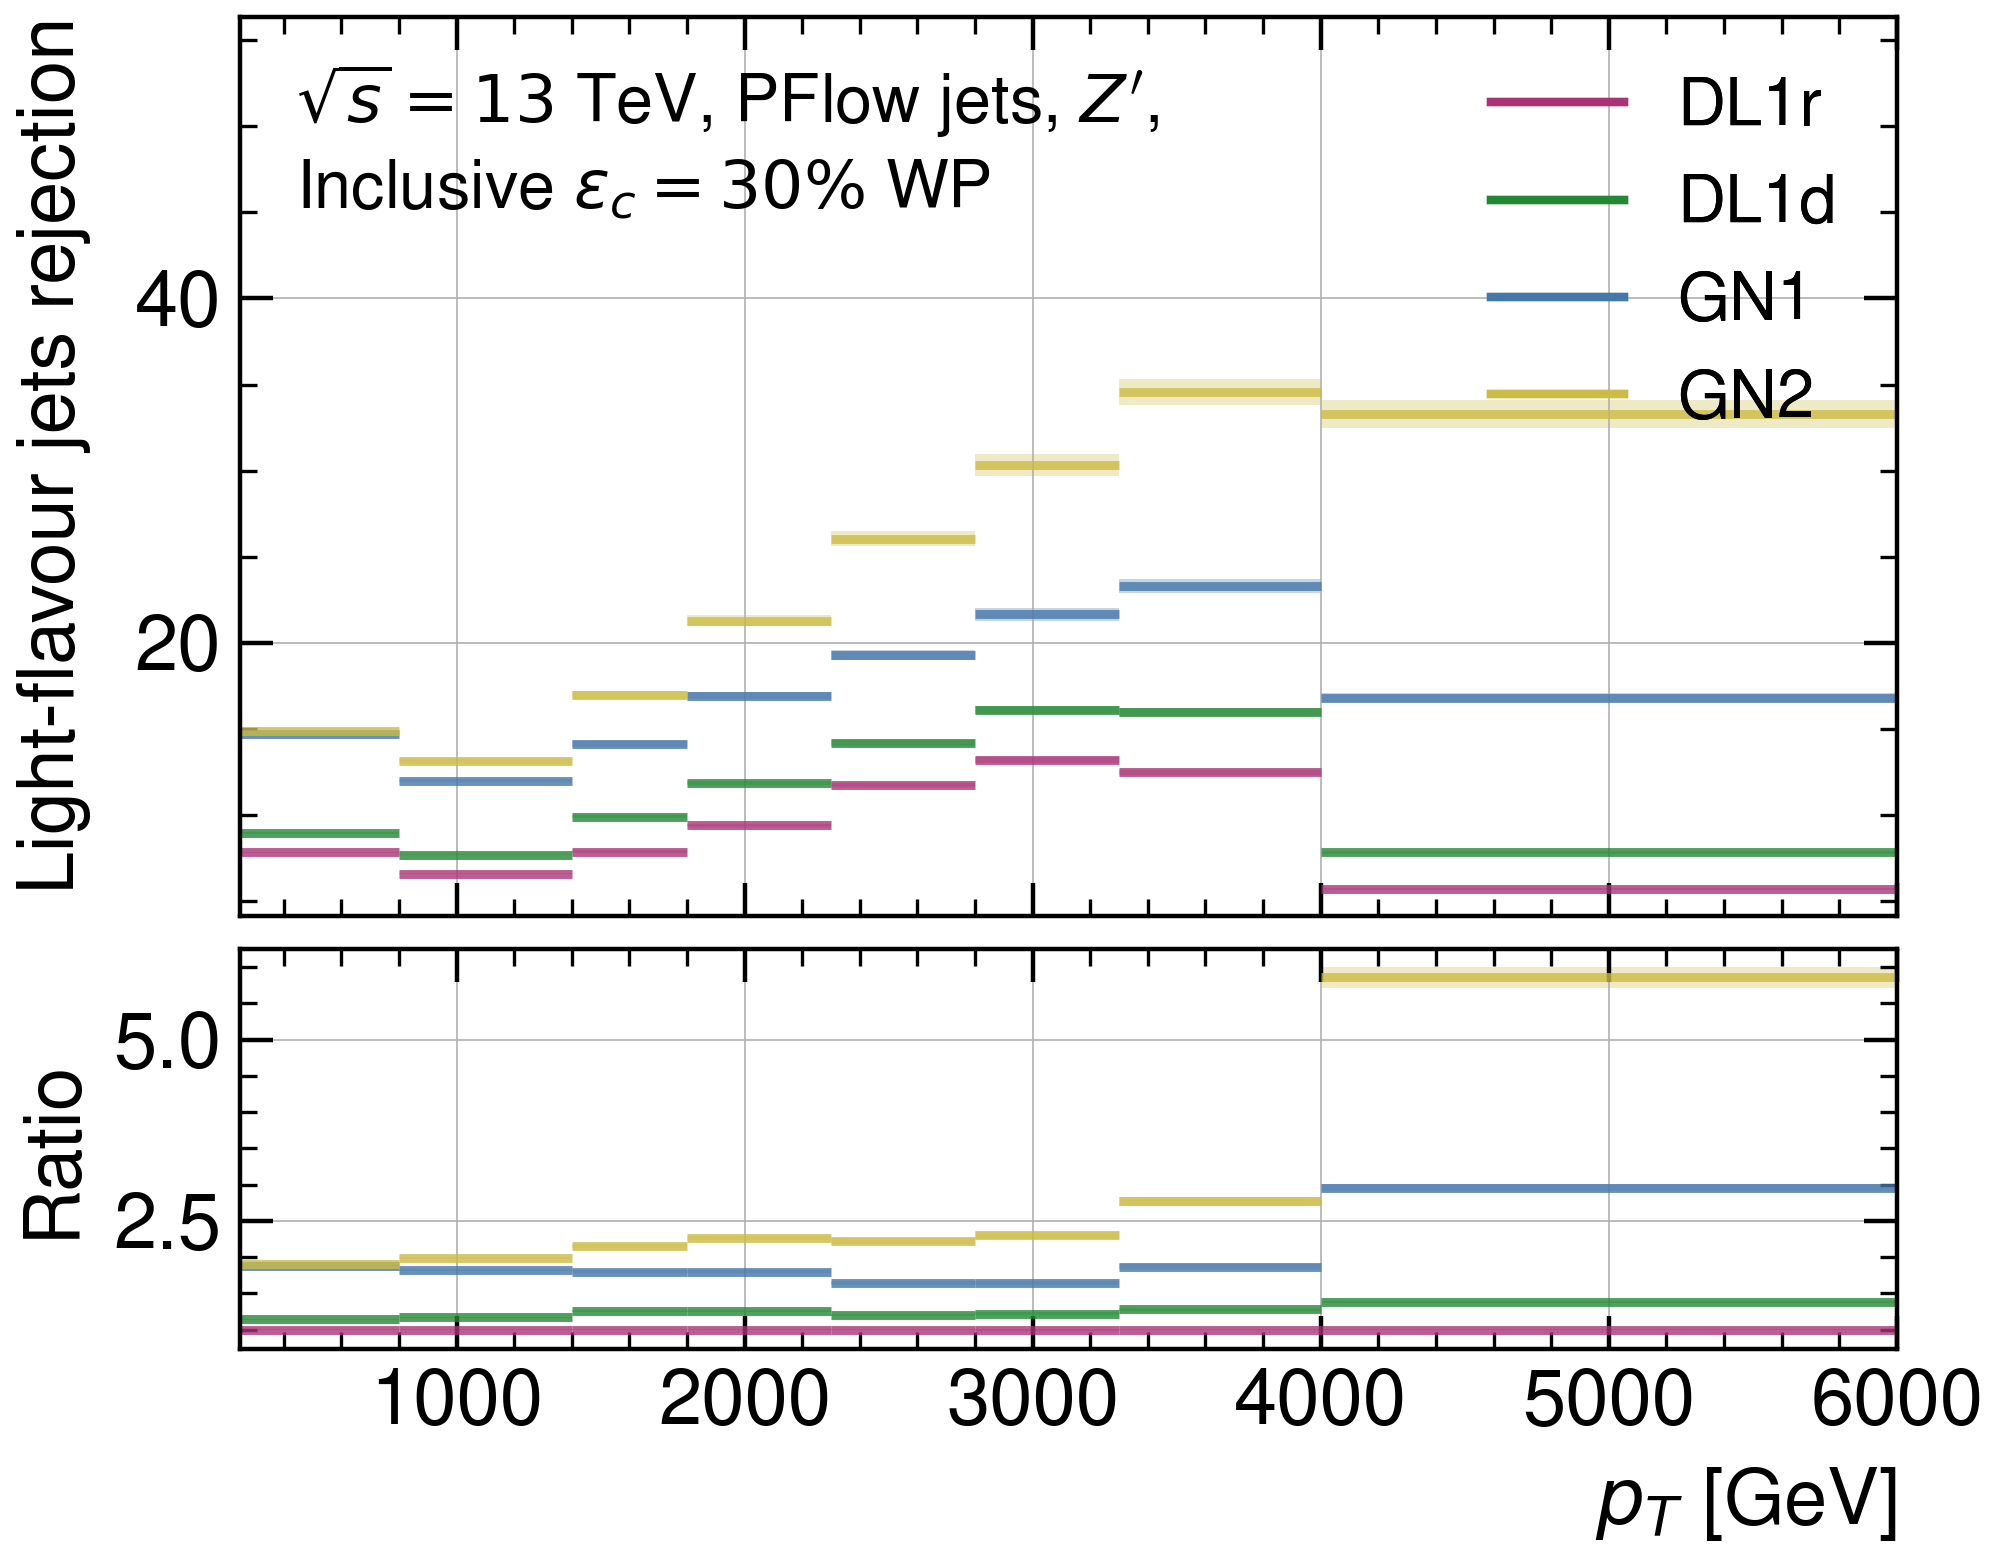
\includegraphics[width=0.48\textwidth]{Images/FTAG/GN/GN2/pt_plots/pt_zp_light_rej_c.png}
    \caption{Comparing the different models light-rejection as a function of jet $p_T$ for the $c$-tagging inclusive 30\% working point on the $t\bar{t}$ (left) and  $Z'$ (right). The flavour fraction is set at $f^c_b = 0.2$ for all taggers.}
    \label{apfig:GNxptc_urej}
  \end{figure} 

  
\newpage
\section{GN2X: GN2 Variant for Boosted Higgs Decays to Heavy Flavours}\label{app-chap-GN2X}
This section presents an interesting application of the \gls{gn2} architecture to a specialised objective: identifying boosted Higgs boson decaying into a pair of $b$- or $c$-quarks. Having an effective tagger to identify these boosted decays can significantly help analyses studying the decay of Higgs particles to a $c\bar{c}$ pair \cite{ATLAS:2022ers}, for the precise measurement of the Higgs boson $p_T$ spectrum \cite{PhysRevD.105.092003}, and for beyond the \gls{sm} measurements \cite{ATLAS:2023azi}. To perform this task, a new algorithm labelled GN2X is introduced based on the design of \gls{gn2} \cite{ATL-PHYS-PUB-2023-021}. Its main task is to discriminate jets from boosted Higgs boson decaying into a $b\bar{b}$ or a $c\bar{c}$ pair from those originating from the fully-hadronic top-quark decay and the multi-jet processes. While other taggers presented in this chapter relied on small-radius ($R=0.4$) PFlow jets or \gls{vr} jets, GN2X is trained on jet reconstructed with a large-radius ($R=1.0$) with \gls{ufo} objects to capture the majority of the decay products \cite{atlasLARGERJet}. \gls{ufo} combines PFlow \cite{atlasPFLOW} and Track-Calo clusters objects \cite{ATL-PHYS-PUB-2017-015}, thereby including neutral and charged components in the reconstruction. \gls{ufo} large-$R$ jets are reconstructed with the anti-$k_T$ algorithm with a radius $R = 1.0$ \cite{Cacciari:2008gp}. \\

To train the algorithm, Higgs produced in association with a $Z$-boson and decaying to a pair of heavy flavour quarks ($b\bar{b}$ or a $c\bar{c}$) are simulated. To not bias the result towards a specific $p_T$, $\eta$, and mass distributions of the jets, the simulations are resampled to have an approximately flat distribution of jet mass in the training set, while the validation set follows the \gls{sm} $ZH$ production for a Higgs boson $H$ of a mass equal to 125 GeV. Similarly, the top-quark decay with subsequent hadronic decay of the $W$ boson in the $t \rightarrow bW$ chain is simulated for the training samples using a hypothetical $Z'$-boson of 4 TeV mass decaying as $Z' \rightarrow t\bar(t)$ with approximately flat jet $p_T$ distribution. The evaluation sample uses the \gls{sm} $t\bar{t}$ decay with filters on the scalar sum of the objects $p_T$ in the event. Finally, the multi-jet process is simulated in slices of particle-level jet $p_T$ to have the same spectrum. More details on the simulated samples used can be found in Ref. \cite{ATL-PHYS-PUB-2023-021}. After resampling the samples to enforce the same $p_T$, $\eta$, and mass distributions, there are 62 million jets split between 15 million $H_{b\bar{b}}$, 15 million $H_{c\bar{c}}$, 10 million top, and 22 million multi-jets. \\

The previous algorithm for this task that now serves as benchmark in this study is the $X_{bb}$ tagger, a feed-forward network combining the flavour tagging discriminants of \gls{dl1r} or \gls{dl1d} for up to three \gls{vr} sub-jets associated to the large-$R$ jet \cite{ATL-PHYS-PUB-2020-019, ATL-PHYS-PUB-2021-035}. The track selection is similar to that of the GN-models (Section \ref{chap:GN}), and the inputs of the model are equivalent to those of Table~\ref{tab:gnInputVariables}, with the jet variables defined on the large-$R$ jet with the addition of the mass of the large-$R$ jet. At most 100 tracks associated with a jet are supplied to the network, as sorted by the decreasing transverse impact parameter significance $S_{d_0}$. The same auxiliary tasks as in \gls{gn2} are used with the same respective weights and neural network designs. The initialiser has a 192 embedding dimension and the transformer encoder combines 6 layers with 4 attention heads. The global representation is again obtained from an attention-weighted sum over the conditional tracks, with learnable attention weights. GN2X contains in total 1.5 million parameters and is trained on 4 A100 \glspl{gpu} for 40 epochs ($\sim$1 hour per epoch) with a batchsize of 1000. \\

The model outputs four probabilities $p_{H_{b\bar{b}}}$, $p_{H_{c\bar{c}}}$, $p_{\textrm{top}}$, and $p_{\textrm{QCD}}$ that are combined in a discriminant score equivalent to Equations \ref{bdisc} and \ref{cdisc}: 
\begin{equation}
  D_{H_{b\bar{b}}} = \log \frac{p_{H_{b\bar{b}}}}{f_{H_{c\bar{c}}} . p_{H_{c\bar{c}}} + f_{\textrm{top}} . p_{\textrm{top}} + (1 - f_{H_{c\bar{c}}} - f_{\textrm{top}}) . p_{\textrm{QCD}}},
\end{equation}
where the flavour fractions were chosen from dedicated performance studies to be $f_{H_{c\bar{c}}} = 0.02$ and $f_{\textrm{top}} = 0.25$. A discriminant for $H_{c\bar{c}}$ is similarly defined with $f_{H_{b\bar{b}}} = 0.3$ and $f_{\textrm{top}} = 0.25$:
\begin{equation}
  D_{H_{c\bar{c}}} = \log \frac{p_{H_{c\bar{c}}}}{f_{H_{b\bar{b}}} . p_{H_{b\bar{b}}} + f_{\textrm{top}} . p_{\textrm{top}} + (1 - f_{H_{b\bar{b}}} - f_{\textrm{top}}) . p_{\textrm{QCD}}}.
\end{equation}

The performance of GN2X can be assessed from the \gls{roc} curves presented in Figure~\ref{fig:rocGN2X}. An additional performance to $X_{bb}$ and GN2X is presented, where two individual \gls{vr} sub-jets are $b$- or $c$-tagged by a \gls{vr}-trained \gls{gn2} model. The jets used are the leading \gls{vr} sub-jets associated with the large-$R$ jet. Note that $X_{bb}$ was not retrained on the specific samples but uses the \gls{vr}-trained \gls{dl1d} previously introduced. A clear performance gained is delivered by the GN2X method above both the $X_{bb}$ tagger and the combination of two individual tags with \gls{gn2}. The latter approach does not access correlations between the sub-jets, explaining its lower performance at higher $H(b\bar{b})$ and $H(c\bar{c})$ efficiencies than the GN2X and $X_{bb}$ model. At a 50\% $H(b\bar{b})$ \gls{wp}, GN2X improves the top rejection (multi-jet rejection) on $X_{bb}$ by a factor 1.6 (2.5) \cite{ATL-PHYS-PUB-2023-021}. For $H(b\bar{b})$ tagging, the $H(c\bar{c})$ background is negligible. GN2X also improves the performance for $H(c\bar{c})$ tagging over the approach combining two individual \gls{vr} tagged-jets: at a 50\% \gls{wp}, GN2X improves the top rejection by a factor 3, the multi-jet rejection by a factor 5, and the $H(b\bar{b})$ rejection by a factor 6. This novel approach to perform boosted object tagging is the first of its kind in ATLAS and is now integrated into the ATLAS software.

\begin{center}
  \begin{figure}[h!]
  \centerline{
  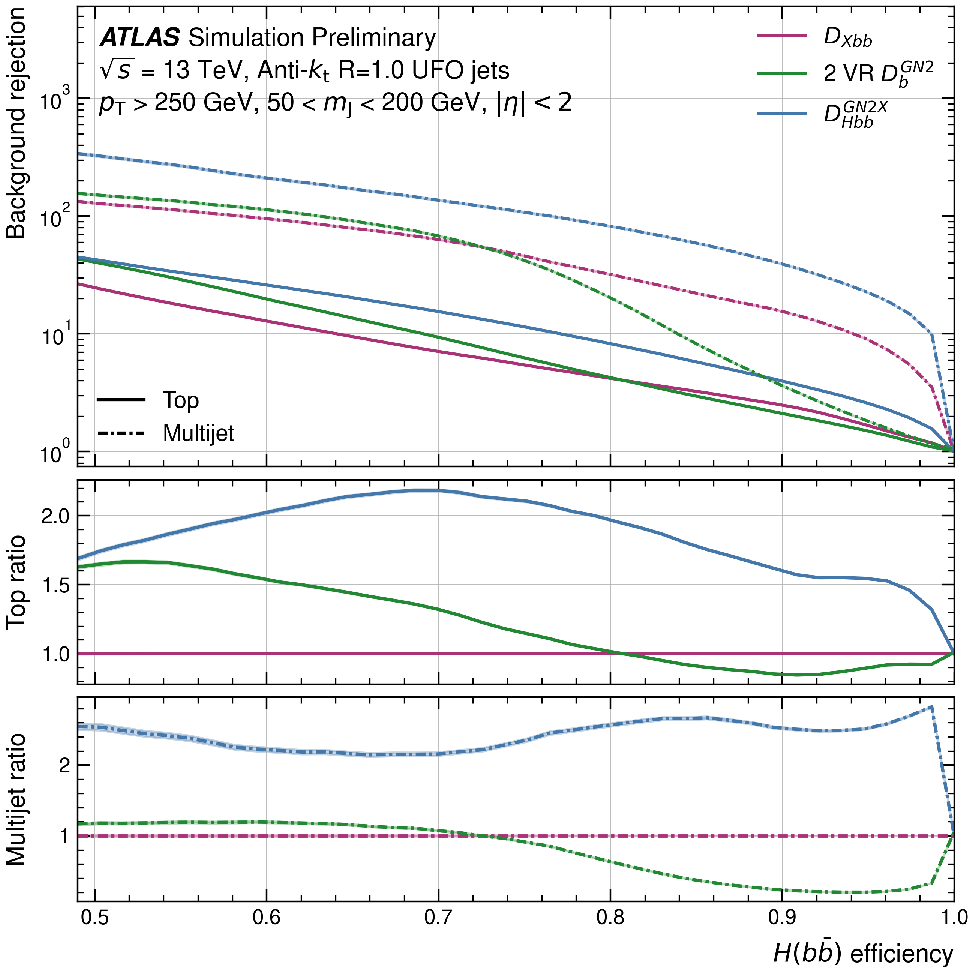
\includegraphics[width=0.50\textwidth]{Images/FTAG/GN2X/roc/rocHbb.pdf}
  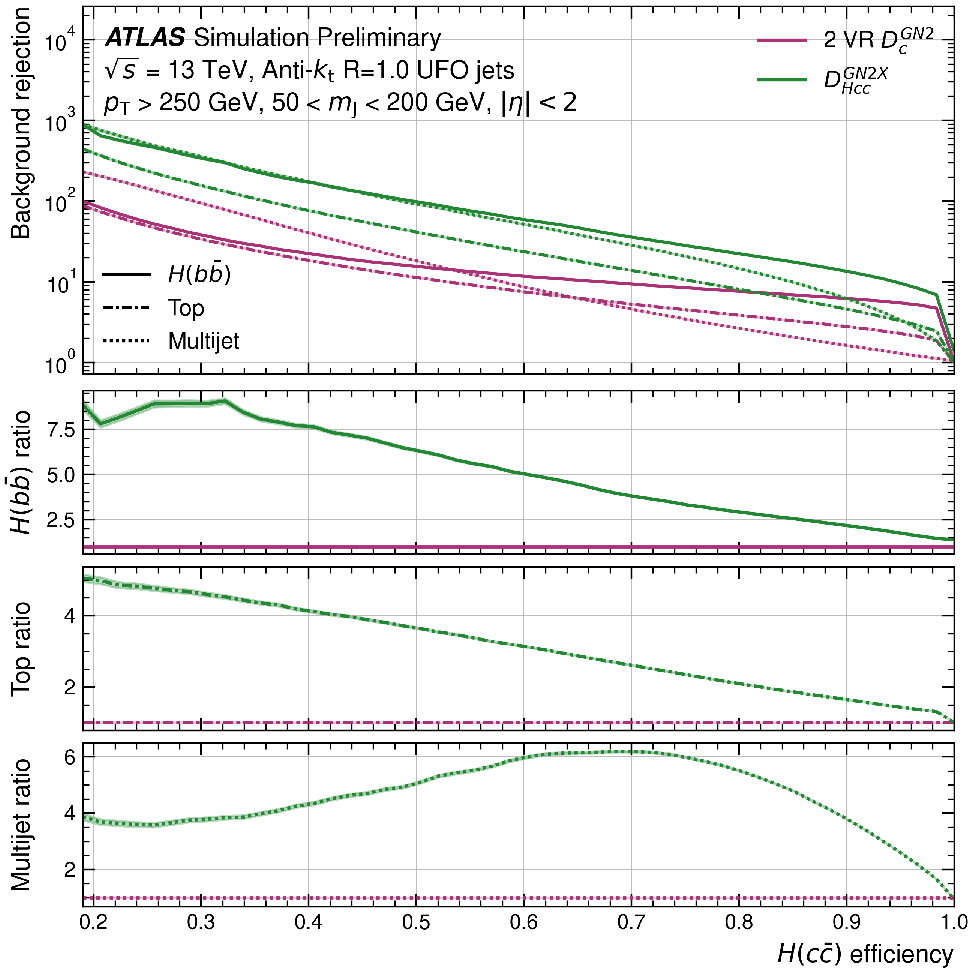
\includegraphics[width=0.50\textwidth]{Images/FTAG/GN2X/roc/rocHcc.pdf}
  }
  \caption{The ROC curves for $H(b\bar{b})$ (left) and $H(c\bar{c})$ tagging (right) on an SM simulated test samples \cite{ATL-PHYS-PUB-2023-021}. The respective tagging efficiency is displayed versus the top and multi-jet rejections, for jets with a $p_T > 250$ GeV and a mass $50 < m_J < 200$ GeV. Models compared are the baseline $X_{bb}$ tagger, using the variable-radius DL1r of at most 3 identified sub-jets in the large-$R$ jet, the tag obtained by combining the tag on two variable-radius jets within the large-$R$ jet with the single-jet GN2 tagger, and the GN2X model. The former is only available for $H(b\bar{b})$ tagging, and the $H(b\bar{b})$ rejection is displayed for $H(c\bar{c})$ tagging. The $H(c\bar{c})$ background is negligible for $H(b\bar{b})$ tagging. Shaded regions represent the binominal error band.}
  \label{fig:rocGN2X}
  \end{figure}
\end{center}